\subsubsection{E0A [2H2L]}
\label{apx:E0A:2H2L}

\begin{multicols}{2}
\begin{center}
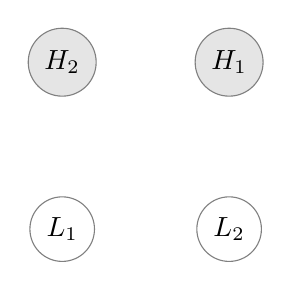
\begin{tikzpicture}[shorten >=1pt,draw=black!50]
	\node (H1) at ( 1.06,  1.06)	[circle, draw, fill = gray!20]	{$H_{1}$};
	\node (H2) at (-1.06,  1.06)	[circle, draw, fill = gray!20]	{$H_{2}$};
	\node (L1) at (-1.06, -1.06)	[circle, draw, fill = white]	{$L_{1}$};
	\node (L2) at ( 1.06, -1.06)	[circle, draw, fill = white]	{$L_{2}$};
\end{tikzpicture}
\end{center}
\columnbreak

\scaleeq{
Equations: \begin{cases}
	e^{H}_{1} \left(\frac{25 \phi}{4} - 4\right) = \alpha - e^{H}_{2} - e^{L}_{1} \theta - e^{L}_{2} \theta - \gamma\\
	e^{H}_{2} \left(\frac{25 \phi}{4} - 4\right) = \alpha - e^{H}_{1} - e^{L}_{1} \theta - e^{L}_{2} \theta - \gamma\\
	e^{L}_{1} \left(\frac{25 \phi}{4 \theta} - 4 \theta\right) = \alpha - e^{H}_{1} - e^{H}_{2} - e^{L}_{2} \theta - \gamma\\
	e^{L}_{2} \left(\frac{25 \phi}{4 \theta} - 4 \theta\right) = \alpha - e^{H}_{1} - e^{H}_{2} - e^{L}_{1} \theta - \gamma
\end{cases}
}\end{multicols}


Optimal efforts:

\scaleeq{
\begin{cases}
	e^{H}_{1} &= \frac{4 \left(\alpha - \gamma\right) \left(5 \phi - 4 \theta^{2}\right)}{125 \phi^{2} - 60 \phi \theta^{2} - 60 \phi + 16 \theta^{2}}\\
	e^{H}_{2} &= \frac{4 \left(\alpha - \gamma\right) \left(5 \phi - 4 \theta^{2}\right)}{125 \phi^{2} - 60 \phi \theta^{2} - 60 \phi + 16 \theta^{2}}\\
	e^{L}_{1} &= \frac{4 \theta \left(\alpha - \gamma\right) \left(5 \phi - 4\right)}{125 \phi^{2} - 60 \phi \theta^{2} - 60 \phi + 16 \theta^{2}}\\
	e^{L}_{2} &= \frac{4 \theta \left(\alpha - \gamma\right) \left(5 \phi - 4\right)}{125 \phi^{2} - 60 \phi \theta^{2} - 60 \phi + 16 \theta^{2}}
\end{cases}
}

Production Costs:

\scaleeq{
\begin{cases}
	c^{H}_{1} &= - \frac{20 \alpha \phi - 16 \alpha \theta^{2} - 125 \gamma \phi^{2} + 60 \gamma \phi \theta^{2} + 40 \gamma \phi}{125 \phi^{2} - 60 \phi \theta^{2} - 60 \phi + 16 \theta^{2}}\\
	c^{H}_{2} &= - \frac{20 \alpha \phi - 16 \alpha \theta^{2} - 125 \gamma \phi^{2} + 60 \gamma \phi \theta^{2} + 40 \gamma \phi}{125 \phi^{2} - 60 \phi \theta^{2} - 60 \phi + 16 \theta^{2}}\\
	c^{L}_{1} &= - \frac{20 \alpha \phi \theta^{2} - 16 \alpha \theta^{2} - 125 \gamma \phi^{2} + 40 \gamma \phi \theta^{2} + 60 \gamma \phi}{125 \phi^{2} - 60 \phi \theta^{2} - 60 \phi + 16 \theta^{2}}\\
	c^{L}_{2} &= - \frac{20 \alpha \phi \theta^{2} - 16 \alpha \theta^{2} - 125 \gamma \phi^{2} + 40 \gamma \phi \theta^{2} + 60 \gamma \phi}{125 \phi^{2} - 60 \phi \theta^{2} - 60 \phi + 16 \theta^{2}}
\end{cases}
}

Production Quantities:

\scaleeq{
\begin{cases}
	q^{H}_{1} &= \frac{5 \phi \left(\alpha - \gamma\right) \left(5 \phi - 4 \theta^{2}\right)}{125 \phi^{2} - 60 \phi \theta^{2} - 60 \phi + 16 \theta^{2}}\\
	q^{H}_{2} &= \frac{5 \phi \left(\alpha - \gamma\right) \left(5 \phi - 4 \theta^{2}\right)}{125 \phi^{2} - 60 \phi \theta^{2} - 60 \phi + 16 \theta^{2}}\\
	q^{L}_{1} &= \frac{5 \phi \left(\alpha - \gamma\right) \left(5 \phi - 4\right)}{125 \phi^{2} - 60 \phi \theta^{2} - 60 \phi + 16 \theta^{2}}\\
	q^{L}_{2} &= \frac{5 \phi \left(\alpha - \gamma\right) \left(5 \phi - 4\right)}{125 \phi^{2} - 60 \phi \theta^{2} - 60 \phi + 16 \theta^{2}}
\end{cases}
}

Profits:

\begin{equation}
\label{eq:E0A:2H2L_profit}
\scaledequation{\begin{cases}
	\pi^{H}_{1} &= \frac{\phi \left(\alpha - \gamma\right)^{2} \left(5 \phi - 4 \theta^{2}\right)^{2} \left(25 \phi - 16\right)}{\left(125 \phi^{2} - 60 \phi \theta^{2} - 60 \phi + 16 \theta^{2}\right)^{2}}\\
	\pi^{H}_{2} &= \frac{\phi \left(\alpha - \gamma\right)^{2} \left(5 \phi - 4 \theta^{2}\right)^{2} \left(25 \phi - 16\right)}{\left(125 \phi^{2} - 60 \phi \theta^{2} - 60 \phi + 16 \theta^{2}\right)^{2}}\\
	\pi^{L}_{1} &= \frac{\phi \left(\alpha - \gamma\right)^{2} \left(5 \phi - 4\right)^{2} \left(25 \phi - 16 \theta^{2}\right)}{\left(125 \phi^{2} - 60 \phi \theta^{2} - 60 \phi + 16 \theta^{2}\right)^{2}}\\
	\pi^{L}_{2} &= \frac{\phi \left(\alpha - \gamma\right)^{2} \left(5 \phi - 4\right)^{2} \left(25 \phi - 16 \theta^{2}\right)}{\left(125 \phi^{2} - 60 \phi \theta^{2} - 60 \phi + 16 \theta^{2}\right)^{2}}
\end{cases}
}
\end{equation}

Total Production:

\scaleeq{
\frac{20 \phi \left(\alpha - \gamma\right) \left(5 \phi - 2 \theta^{2} - 2\right)}{125 \phi^{2} - 60 \phi \theta^{2} - 60 \phi + 16 \theta^{2}}
}

Price:

\scaleeq{
\frac{25 \alpha \phi^{2} - 20 \alpha \phi \theta^{2} - 20 \alpha \phi + 16 \alpha \theta^{2} + 100 \gamma \phi^{2} - 40 \gamma \phi \theta^{2} - 40 \gamma \phi}{125 \phi^{2} - 60 \phi \theta^{2} - 60 \phi + 16 \theta^{2}}
}

Firm Surplus:

\scaleeq{
\frac{4 \phi \left(\alpha - \gamma\right)^{2} \left(625 \phi^{3} - 700 \phi^{2} \theta^{2} - 700 \phi^{2} + 200 \phi \theta^{4} + 640 \phi \theta^{2} + 200 \phi - 128 \theta^{4} - 128 \theta^{2}\right)}{\left(125 \phi^{2} - 60 \phi \theta^{2} - 60 \phi + 16 \theta^{2}\right)^{2}}
}

Consumer Surplus:

\scaleeq{
\frac{200 \phi^{2} \left(\alpha - \gamma\right)^{2} \left(5 \phi - 2 \theta^{2} - 2\right)^{2}}{\left(125 \phi^{2} - 60 \phi \theta^{2} - 60 \phi + 16 \theta^{2}\right)^{2}}
}

Social Welfare:

\scaleeq{
\frac{4 \phi \left(\alpha - \gamma\right)^{2} \left(1875 \phi^{3} - 1700 \phi^{2} \theta^{2} - 1700 \phi^{2} + 400 \phi \theta^{4} + 1040 \phi \theta^{2} + 400 \phi - 128 \theta^{4} - 128 \theta^{2}\right)}{\left(125 \phi^{2} - 60 \phi \theta^{2} - 60 \phi + 16 \theta^{2}\right)^{2}}
}

%======================================================================

\subsubsection{E1A [2H2L]}
\label{apx:E1A:2H2L}

\begin{multicols}{2}
\begin{center}
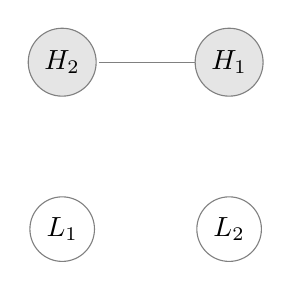
\begin{tikzpicture}[shorten >=1pt,draw=black!50]
	\node (H1) at ( 1.06,  1.06)	[circle, draw, fill = gray!20]	{$H_{1}$};
	\node (H2) at (-1.06,  1.06)	[circle, draw, fill = gray!20]	{$H_{2}$};
	\node (L1) at (-1.06, -1.06)	[circle, draw, fill = white]	{$L_{1}$};
	\node (L2) at ( 1.06, -1.06)	[circle, draw, fill = white]	{$L_{2}$};
	\draw (H1) -- (H2);
\end{tikzpicture}
\end{center}
\columnbreak

\scaleeq{
Equations: \begin{cases}
	e^{H}_{1} \left(\frac{25 \phi}{3} - 3\right) = \alpha + 3 e^{H}_{2} - e^{L}_{1} \theta - e^{L}_{2} \theta - \gamma\\
	e^{H}_{2} \left(\frac{25 \phi}{3} - 3\right) = \alpha + 3 e^{H}_{1} - e^{L}_{1} \theta - e^{L}_{2} \theta - \gamma\\
	e^{L}_{1} \left(\frac{25 \phi}{4 \theta} - 4 \theta\right) = \alpha - 2 e^{H}_{1} - 2 e^{H}_{2} - e^{L}_{2} \theta - \gamma\\
	e^{L}_{2} \left(\frac{25 \phi}{4 \theta} - 4 \theta\right) = \alpha - 2 e^{H}_{1} - 2 e^{H}_{2} - e^{L}_{1} \theta - \gamma
\end{cases}
}\end{multicols}


Optimal efforts:

\scaleeq{
\begin{cases}
	e^{H}_{1} &= \frac{3 \left(\alpha - \gamma\right) \left(5 \phi - 4 \theta^{2}\right)}{125 \phi^{2} - 60 \phi \theta^{2} - 90 \phi + 24 \theta^{2}}\\
	e^{H}_{2} &= \frac{3 \left(\alpha - \gamma\right) \left(5 \phi - 4 \theta^{2}\right)}{125 \phi^{2} - 60 \phi \theta^{2} - 90 \phi + 24 \theta^{2}}\\
	e^{L}_{1} &= \frac{4 \theta \left(\alpha - \gamma\right) \left(5 \phi - 6\right)}{125 \phi^{2} - 60 \phi \theta^{2} - 90 \phi + 24 \theta^{2}}\\
	e^{L}_{2} &= \frac{4 \theta \left(\alpha - \gamma\right) \left(5 \phi - 6\right)}{125 \phi^{2} - 60 \phi \theta^{2} - 90 \phi + 24 \theta^{2}}
\end{cases}
}

Production Costs:

\scaleeq{
\begin{cases}
	c^{H}_{1} &= - \frac{30 \alpha \phi - 24 \alpha \theta^{2} - 125 \gamma \phi^{2} + 60 \gamma \phi \theta^{2} + 60 \gamma \phi}{125 \phi^{2} - 60 \phi \theta^{2} - 90 \phi + 24 \theta^{2}}\\
	c^{H}_{2} &= - \frac{30 \alpha \phi - 24 \alpha \theta^{2} - 125 \gamma \phi^{2} + 60 \gamma \phi \theta^{2} + 60 \gamma \phi}{125 \phi^{2} - 60 \phi \theta^{2} - 90 \phi + 24 \theta^{2}}\\
	c^{L}_{1} &= - \frac{20 \alpha \phi \theta^{2} - 24 \alpha \theta^{2} - 125 \gamma \phi^{2} + 40 \gamma \phi \theta^{2} + 90 \gamma \phi}{125 \phi^{2} - 60 \phi \theta^{2} - 90 \phi + 24 \theta^{2}}\\
	c^{L}_{2} &= - \frac{20 \alpha \phi \theta^{2} - 24 \alpha \theta^{2} - 125 \gamma \phi^{2} + 40 \gamma \phi \theta^{2} + 90 \gamma \phi}{125 \phi^{2} - 60 \phi \theta^{2} - 90 \phi + 24 \theta^{2}}
\end{cases}
}

Production Quantities:

\scaleeq{
\begin{cases}
	q^{H}_{1} &= \frac{5 \phi \left(\alpha - \gamma\right) \left(5 \phi - 4 \theta^{2}\right)}{125 \phi^{2} - 60 \phi \theta^{2} - 90 \phi + 24 \theta^{2}}\\
	q^{H}_{2} &= \frac{5 \phi \left(\alpha - \gamma\right) \left(5 \phi - 4 \theta^{2}\right)}{125 \phi^{2} - 60 \phi \theta^{2} - 90 \phi + 24 \theta^{2}}\\
	q^{L}_{1} &= \frac{5 \phi \left(\alpha - \gamma\right) \left(5 \phi - 6\right)}{125 \phi^{2} - 60 \phi \theta^{2} - 90 \phi + 24 \theta^{2}}\\
	q^{L}_{2} &= \frac{5 \phi \left(\alpha - \gamma\right) \left(5 \phi - 6\right)}{125 \phi^{2} - 60 \phi \theta^{2} - 90 \phi + 24 \theta^{2}}
\end{cases}
}

Profits:

\begin{equation}
\label{eq:E1A:2H2L_profit}
\scaledequation{\begin{cases}
	\pi^{H}_{1} &= \frac{\phi \left(\alpha - \gamma\right)^{2} \left(5 \phi - 4 \theta^{2}\right)^{2} \left(25 \phi - 9\right)}{\left(125 \phi^{2} - 60 \phi \theta^{2} - 90 \phi + 24 \theta^{2}\right)^{2}}\\
	\pi^{H}_{2} &= \frac{\phi \left(\alpha - \gamma\right)^{2} \left(5 \phi - 4 \theta^{2}\right)^{2} \left(25 \phi - 9\right)}{\left(125 \phi^{2} - 60 \phi \theta^{2} - 90 \phi + 24 \theta^{2}\right)^{2}}\\
	\pi^{L}_{1} &= \frac{\phi \left(\alpha - \gamma\right)^{2} \left(5 \phi - 6\right)^{2} \left(25 \phi - 16 \theta^{2}\right)}{\left(125 \phi^{2} - 60 \phi \theta^{2} - 90 \phi + 24 \theta^{2}\right)^{2}}\\
	\pi^{L}_{2} &= \frac{\phi \left(\alpha - \gamma\right)^{2} \left(5 \phi - 6\right)^{2} \left(25 \phi - 16 \theta^{2}\right)}{\left(125 \phi^{2} - 60 \phi \theta^{2} - 90 \phi + 24 \theta^{2}\right)^{2}}
\end{cases}
}
\end{equation}

Total Production:

\scaleeq{
\frac{20 \phi \left(\alpha - \gamma\right) \left(5 \phi - 2 \theta^{2} - 3\right)}{125 \phi^{2} - 60 \phi \theta^{2} - 90 \phi + 24 \theta^{2}}
}

Price:

\scaleeq{
\frac{25 \alpha \phi^{2} - 20 \alpha \phi \theta^{2} - 30 \alpha \phi + 24 \alpha \theta^{2} + 100 \gamma \phi^{2} - 40 \gamma \phi \theta^{2} - 60 \gamma \phi}{125 \phi^{2} - 60 \phi \theta^{2} - 90 \phi + 24 \theta^{2}}
}

Firm Surplus:

\scaleeq{
\frac{2 \phi \left(\alpha - \gamma\right)^{2} \left(1250 \phi^{3} - 1400 \phi^{2} \theta^{2} - 1725 \phi^{2} + 400 \phi \theta^{4} + 1320 \phi \theta^{2} + 900 \phi - 144 \theta^{4} - 576 \theta^{2}\right)}{\left(125 \phi^{2} - 60 \phi \theta^{2} - 90 \phi + 24 \theta^{2}\right)^{2}}
}

Consumer Surplus:

\scaleeq{
\frac{200 \phi^{2} \left(\alpha - \gamma\right)^{2} \left(5 \phi - 2 \theta^{2} - 3\right)^{2}}{\left(125 \phi^{2} - 60 \phi \theta^{2} - 90 \phi + 24 \theta^{2}\right)^{2}}
}

Social Welfare:

\scaleeq{
\frac{2 \phi \left(\alpha - \gamma\right)^{2} \left(3750 \phi^{3} - 3400 \phi^{2} \theta^{2} - 4725 \phi^{2} + 800 \phi \theta^{4} + 2520 \phi \theta^{2} + 1800 \phi - 144 \theta^{4} - 576 \theta^{2}\right)}{\left(125 \phi^{2} - 60 \phi \theta^{2} - 90 \phi + 24 \theta^{2}\right)^{2}}
}

%======================================================================

\subsubsection{E1B [2H2L]}
\label{apx:E1B:2H2L}

\begin{multicols}{2}
\begin{center}
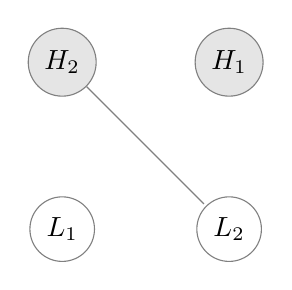
\begin{tikzpicture}[shorten >=1pt,draw=black!50]
	\node (H1) at ( 1.06,  1.06)	[circle, draw, fill = gray!20]	{$H_{1}$};
	\node (H2) at (-1.06,  1.06)	[circle, draw, fill = gray!20]	{$H_{2}$};
	\node (L1) at (-1.06, -1.06)	[circle, draw, fill = white]	{$L_{1}$};
	\node (L2) at ( 1.06, -1.06)	[circle, draw, fill = white]	{$L_{2}$};
	\draw (H2) -- (L2);
\end{tikzpicture}
\end{center}
\columnbreak

\scaleeq{
Equations: \begin{cases}
	e^{H}_{1} \left(\frac{25 \phi}{4} - 4\right) = \alpha - 2 e^{H}_{2} - e^{L}_{1} \theta - 2 e^{L}_{2} \theta - \gamma\\
	e^{H}_{2} \left(\frac{25 \phi}{3} - 3\right) = \alpha - e^{H}_{1} - e^{L}_{1} \theta + 3 e^{L}_{2} \theta - \gamma\\
	e^{L}_{1} \left(\frac{25 \phi}{4 \theta} - 4 \theta\right) = \alpha - e^{H}_{1} - 2 e^{H}_{2} - 2 e^{L}_{2} \theta - \gamma\\
	e^{L}_{2} \left(\frac{25 \phi}{3 \theta} - 3 \theta\right) = \alpha - e^{H}_{1} + 3 e^{H}_{2} - e^{L}_{1} \theta - \gamma
\end{cases}
}\end{multicols}


Optimal efforts:

\scaleeq{
\begin{cases}
	e^{H}_{1} &= \frac{4 \left(\alpha - \gamma\right) \left(5 \phi - 4 \theta^{2}\right) \left(5 \phi - 3 \theta^{2} - 3\right)}{625 \phi^{3} - 625 \phi^{2} \theta^{2} - 625 \phi^{2} + 120 \phi \theta^{4} + 480 \phi \theta^{2} + 120 \phi - 48 \theta^{4} - 48 \theta^{2}}\\
	e^{H}_{2} &= \frac{3 \left(\alpha - \gamma\right) \left(5 \phi - 4\right) \left(5 \phi - 4 \theta^{2}\right)}{625 \phi^{3} - 625 \phi^{2} \theta^{2} - 625 \phi^{2} + 120 \phi \theta^{4} + 480 \phi \theta^{2} + 120 \phi - 48 \theta^{4} - 48 \theta^{2}}\\
	e^{L}_{1} &= \frac{4 \theta \left(\alpha - \gamma\right) \left(5 \phi - 4\right) \left(5 \phi - 3 \theta^{2} - 3\right)}{625 \phi^{3} - 625 \phi^{2} \theta^{2} - 625 \phi^{2} + 120 \phi \theta^{4} + 480 \phi \theta^{2} + 120 \phi - 48 \theta^{4} - 48 \theta^{2}}\\
	e^{L}_{2} &= \frac{3 \theta \left(\alpha - \gamma\right) \left(5 \phi - 4\right) \left(5 \phi - 4 \theta^{2}\right)}{625 \phi^{3} - 625 \phi^{2} \theta^{2} - 625 \phi^{2} + 120 \phi \theta^{4} + 480 \phi \theta^{2} + 120 \phi - 48 \theta^{4} - 48 \theta^{2}}
\end{cases}
}

Production Costs:

\scaleeq{
\begin{cases}
	c^{H}_{1} &= - \frac{100 \alpha \phi^{2} - 140 \alpha \phi \theta^{2} - 60 \alpha \phi + 48 \alpha \theta^{4} + 48 \alpha \theta^{2} - 625 \gamma \phi^{3} + 625 \gamma \phi^{2} \theta^{2} + 525 \gamma \phi^{2} - 120 \gamma \phi \theta^{4} - 340 \gamma \phi \theta^{2} - 60 \gamma \phi}{625 \phi^{3} - 625 \phi^{2} \theta^{2} - 625 \phi^{2} + 120 \phi \theta^{4} + 480 \phi \theta^{2} + 120 \phi - 48 \theta^{4} - 48 \theta^{2}}\\
	c^{H}_{2} &= - \frac{75 \alpha \phi^{2} \theta^{2} + 75 \alpha \phi^{2} - 60 \alpha \phi \theta^{4} - 120 \alpha \phi \theta^{2} - 60 \alpha \phi + 48 \alpha \theta^{4} + 48 \alpha \theta^{2} - 625 \gamma \phi^{3} + 550 \gamma \phi^{2} \theta^{2} + 550 \gamma \phi^{2} - 60 \gamma \phi \theta^{4} - 360 \gamma \phi \theta^{2} - 60 \gamma \phi}{625 \phi^{3} - 625 \phi^{2} \theta^{2} - 625 \phi^{2} + 120 \phi \theta^{4} + 480 \phi \theta^{2} + 120 \phi - 48 \theta^{4} - 48 \theta^{2}}\\
	c^{L}_{1} &= - \frac{100 \alpha \phi^{2} \theta^{2} - 60 \alpha \phi \theta^{4} - 140 \alpha \phi \theta^{2} + 48 \alpha \theta^{4} + 48 \alpha \theta^{2} - 625 \gamma \phi^{3} + 525 \gamma \phi^{2} \theta^{2} + 625 \gamma \phi^{2} - 60 \gamma \phi \theta^{4} - 340 \gamma \phi \theta^{2} - 120 \gamma \phi}{625 \phi^{3} - 625 \phi^{2} \theta^{2} - 625 \phi^{2} + 120 \phi \theta^{4} + 480 \phi \theta^{2} + 120 \phi - 48 \theta^{4} - 48 \theta^{2}}\\
	c^{L}_{2} &= - \frac{75 \alpha \phi^{2} \theta^{2} + 75 \alpha \phi^{2} - 60 \alpha \phi \theta^{4} - 120 \alpha \phi \theta^{2} - 60 \alpha \phi + 48 \alpha \theta^{4} + 48 \alpha \theta^{2} - 625 \gamma \phi^{3} + 550 \gamma \phi^{2} \theta^{2} + 550 \gamma \phi^{2} - 60 \gamma \phi \theta^{4} - 360 \gamma \phi \theta^{2} - 60 \gamma \phi}{625 \phi^{3} - 625 \phi^{2} \theta^{2} - 625 \phi^{2} + 120 \phi \theta^{4} + 480 \phi \theta^{2} + 120 \phi - 48 \theta^{4} - 48 \theta^{2}}
\end{cases}
}

Production Quantities:

\scaleeq{
\begin{cases}
	q^{H}_{1} &= \frac{5 \phi \left(\alpha - \gamma\right) \left(5 \phi - 4 \theta^{2}\right) \left(5 \phi - 3 \theta^{2} - 3\right)}{625 \phi^{3} - 625 \phi^{2} \theta^{2} - 625 \phi^{2} + 120 \phi \theta^{4} + 480 \phi \theta^{2} + 120 \phi - 48 \theta^{4} - 48 \theta^{2}}\\
	q^{H}_{2} &= \frac{5 \phi \left(\alpha - \gamma\right) \left(5 \phi - 4\right) \left(5 \phi - 4 \theta^{2}\right)}{625 \phi^{3} - 625 \phi^{2} \theta^{2} - 625 \phi^{2} + 120 \phi \theta^{4} + 480 \phi \theta^{2} + 120 \phi - 48 \theta^{4} - 48 \theta^{2}}\\
	q^{L}_{1} &= \frac{5 \phi \left(\alpha - \gamma\right) \left(5 \phi - 4\right) \left(5 \phi - 3 \theta^{2} - 3\right)}{625 \phi^{3} - 625 \phi^{2} \theta^{2} - 625 \phi^{2} + 120 \phi \theta^{4} + 480 \phi \theta^{2} + 120 \phi - 48 \theta^{4} - 48 \theta^{2}}\\
	q^{L}_{2} &= \frac{5 \phi \left(\alpha - \gamma\right) \left(5 \phi - 4\right) \left(5 \phi - 4 \theta^{2}\right)}{625 \phi^{3} - 625 \phi^{2} \theta^{2} - 625 \phi^{2} + 120 \phi \theta^{4} + 480 \phi \theta^{2} + 120 \phi - 48 \theta^{4} - 48 \theta^{2}}
\end{cases}
}

Profits:

\begin{equation}
\label{eq:E1B:2H2L_profit}
\scaledequation{\begin{cases}
	\pi^{H}_{1} &= \frac{\phi \left(\alpha - \gamma\right)^{2} \left(5 \phi - 4 \theta^{2}\right)^{2} \left(25 \phi - 16\right) \left(5 \phi - 3 \theta^{2} - 3\right)^{2}}{\left(625 \phi^{3} - 625 \phi^{2} \theta^{2} - 625 \phi^{2} + 120 \phi \theta^{4} + 480 \phi \theta^{2} + 120 \phi - 48 \theta^{4} - 48 \theta^{2}\right)^{2}}\\
	\pi^{H}_{2} &= \frac{\phi \left(\alpha - \gamma\right)^{2} \left(5 \phi - 4\right)^{2} \left(5 \phi - 4 \theta^{2}\right)^{2} \left(25 \phi - 9\right)}{\left(625 \phi^{3} - 625 \phi^{2} \theta^{2} - 625 \phi^{2} + 120 \phi \theta^{4} + 480 \phi \theta^{2} + 120 \phi - 48 \theta^{4} - 48 \theta^{2}\right)^{2}}\\
	\pi^{L}_{1} &= \frac{\phi \left(\alpha - \gamma\right)^{2} \left(5 \phi - 4\right)^{2} \left(25 \phi - 16 \theta^{2}\right) \left(5 \phi - 3 \theta^{2} - 3\right)^{2}}{\left(625 \phi^{3} - 625 \phi^{2} \theta^{2} - 625 \phi^{2} + 120 \phi \theta^{4} + 480 \phi \theta^{2} + 120 \phi - 48 \theta^{4} - 48 \theta^{2}\right)^{2}}\\
	\pi^{L}_{2} &= \frac{\phi \left(\alpha - \gamma\right)^{2} \left(5 \phi - 4\right)^{2} \left(5 \phi - 4 \theta^{2}\right)^{2} \left(25 \phi - 9 \theta^{2}\right)}{\left(625 \phi^{3} - 625 \phi^{2} \theta^{2} - 625 \phi^{2} + 120 \phi \theta^{4} + 480 \phi \theta^{2} + 120 \phi - 48 \theta^{4} - 48 \theta^{2}\right)^{2}}
\end{cases}
}
\end{equation}

Total Production:

\scaleeq{
\frac{10 \phi \left(\alpha - \gamma\right) \left(50 \phi^{2} - 45 \phi \theta^{2} - 45 \phi + 6 \theta^{4} + 28 \theta^{2} + 6\right)}{625 \phi^{3} - 625 \phi^{2} \theta^{2} - 625 \phi^{2} + 120 \phi \theta^{4} + 480 \phi \theta^{2} + 120 \phi - 48 \theta^{4} - 48 \theta^{2}}
}

Price:

\scaleeq{
\frac{125 \alpha \phi^{3} - 175 \alpha \phi^{2} \theta^{2} - 175 \alpha \phi^{2} + 60 \alpha \phi \theta^{4} + 200 \alpha \phi \theta^{2} + 60 \alpha \phi - 48 \alpha \theta^{4} - 48 \alpha \theta^{2} + 500 \gamma \phi^{3} - 450 \gamma \phi^{2} \theta^{2} - 450 \gamma \phi^{2} + 60 \gamma \phi \theta^{4} + 280 \gamma \phi \theta^{2} + 60 \gamma \phi}{625 \phi^{3} - 625 \phi^{2} \theta^{2} - 625 \phi^{2} + 120 \phi \theta^{4} + 480 \phi \theta^{2} + 120 \phi - 48 \theta^{4} - 48 \theta^{2}}
}

Firm Surplus:

\scaleeq{
\frac{\phi \left(\alpha - \gamma\right)^{2} \left(62500 \phi^{5} - 128125 \phi^{4} \theta^{2} - 128125 \phi^{4} + 92250 \phi^{3} \theta^{4} + 236500 \phi^{3} \theta^{2} + 92250 \phi^{3} - 28200 \phi^{2} \theta^{6} - 144600 \phi^{2} \theta^{4} - 144600 \phi^{2} \theta^{2} - 28200 \phi^{2} + 3600 \phi \theta^{8} + 32160 \phi \theta^{6} + 69920 \phi \theta^{4} + 32160 \phi \theta^{2} + 3600 \phi - 2304 \theta^{8} - 9216 \theta^{6} - 9216 \theta^{4} - 2304 \theta^{2}\right)}{\left(625 \phi^{3} - 625 \phi^{2} \theta^{2} - 625 \phi^{2} + 120 \phi \theta^{4} + 480 \phi \theta^{2} + 120 \phi - 48 \theta^{4} - 48 \theta^{2}\right)^{2}}
}

Consumer Surplus:

\scaleeq{
\frac{50 \phi^{2} \left(\alpha - \gamma\right)^{2} \left(50 \phi^{2} - 45 \phi \theta^{2} - 45 \phi + 6 \theta^{4} + 28 \theta^{2} + 6\right)^{2}}{\left(625 \phi^{3} - 625 \phi^{2} \theta^{2} - 625 \phi^{2} + 120 \phi \theta^{4} + 480 \phi \theta^{2} + 120 \phi - 48 \theta^{4} - 48 \theta^{2}\right)^{2}}
}

Social Welfare:

\scaleeq{
\frac{\phi \left(\alpha - \gamma\right)^{2} \left(187500 \phi^{5} - 353125 \phi^{4} \theta^{2} - 353125 \phi^{4} + 223500 \phi^{3} \theta^{4} + 579000 \phi^{3} \theta^{2} + 223500 \phi^{3} - 55200 \phi^{2} \theta^{6} - 297600 \phi^{2} \theta^{4} - 297600 \phi^{2} \theta^{2} - 55200 \phi^{2} + 5400 \phi \theta^{8} + 48960 \phi \theta^{6} + 112720 \phi \theta^{4} + 48960 \phi \theta^{2} + 5400 \phi - 2304 \theta^{8} - 9216 \theta^{6} - 9216 \theta^{4} - 2304 \theta^{2}\right)}{\left(625 \phi^{3} - 625 \phi^{2} \theta^{2} - 625 \phi^{2} + 120 \phi \theta^{4} + 480 \phi \theta^{2} + 120 \phi - 48 \theta^{4} - 48 \theta^{2}\right)^{2}}
}

%======================================================================

\subsubsection{E1C [2H2L]}
\label{apx:E1C:2H2L}

\begin{multicols}{2}
\begin{center}
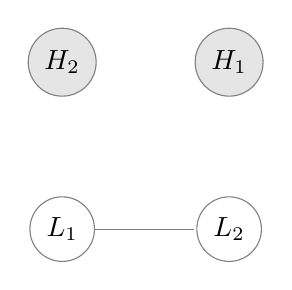
\begin{tikzpicture}[shorten >=1pt,draw=black!50]
	\node (H1) at ( 1.06,  1.06)	[circle, draw, fill = gray!20]	{$H_{1}$};
	\node (H2) at (-1.06,  1.06)	[circle, draw, fill = gray!20]	{$H_{2}$};
	\node (L1) at (-1.06, -1.06)	[circle, draw, fill = white]	{$L_{1}$};
	\node (L2) at ( 1.06, -1.06)	[circle, draw, fill = white]	{$L_{2}$};
	\draw (L1) -- (L2);
\end{tikzpicture}
\end{center}
\columnbreak

\scaleeq{
Equations: \begin{cases}
	e^{H}_{1} \left(\frac{25 \phi}{4} - 4\right) = \alpha - e^{H}_{2} - 2 e^{L}_{1} \theta - 2 e^{L}_{2} \theta - \gamma\\
	e^{H}_{2} \left(\frac{25 \phi}{4} - 4\right) = \alpha - e^{H}_{1} - 2 e^{L}_{1} \theta - 2 e^{L}_{2} \theta - \gamma\\
	e^{L}_{1} \left(\frac{25 \phi}{3 \theta} - 3 \theta\right) = \alpha - e^{H}_{1} - e^{H}_{2} + 3 e^{L}_{2} \theta - \gamma\\
	e^{L}_{2} \left(\frac{25 \phi}{3 \theta} - 3 \theta\right) = \alpha - e^{H}_{1} - e^{H}_{2} + 3 e^{L}_{1} \theta - \gamma
\end{cases}
}\end{multicols}


Optimal efforts:

\scaleeq{
\begin{cases}
	e^{H}_{1} &= \frac{4 \left(\alpha - \gamma\right) \left(5 \phi - 6 \theta^{2}\right)}{125 \phi^{2} - 90 \phi \theta^{2} - 60 \phi + 24 \theta^{2}}\\
	e^{H}_{2} &= \frac{4 \left(\alpha - \gamma\right) \left(5 \phi - 6 \theta^{2}\right)}{125 \phi^{2} - 90 \phi \theta^{2} - 60 \phi + 24 \theta^{2}}\\
	e^{L}_{1} &= \frac{3 \theta \left(\alpha - \gamma\right) \left(5 \phi - 4\right)}{125 \phi^{2} - 90 \phi \theta^{2} - 60 \phi + 24 \theta^{2}}\\
	e^{L}_{2} &= \frac{3 \theta \left(\alpha - \gamma\right) \left(5 \phi - 4\right)}{125 \phi^{2} - 90 \phi \theta^{2} - 60 \phi + 24 \theta^{2}}
\end{cases}
}

Production Costs:

\scaleeq{
\begin{cases}
	c^{H}_{1} &= - \frac{20 \alpha \phi - 24 \alpha \theta^{2} - 125 \gamma \phi^{2} + 90 \gamma \phi \theta^{2} + 40 \gamma \phi}{125 \phi^{2} - 90 \phi \theta^{2} - 60 \phi + 24 \theta^{2}}\\
	c^{H}_{2} &= - \frac{20 \alpha \phi - 24 \alpha \theta^{2} - 125 \gamma \phi^{2} + 90 \gamma \phi \theta^{2} + 40 \gamma \phi}{125 \phi^{2} - 90 \phi \theta^{2} - 60 \phi + 24 \theta^{2}}\\
	c^{L}_{1} &= - \frac{30 \alpha \phi \theta^{2} - 24 \alpha \theta^{2} - 125 \gamma \phi^{2} + 60 \gamma \phi \theta^{2} + 60 \gamma \phi}{125 \phi^{2} - 90 \phi \theta^{2} - 60 \phi + 24 \theta^{2}}\\
	c^{L}_{2} &= - \frac{30 \alpha \phi \theta^{2} - 24 \alpha \theta^{2} - 125 \gamma \phi^{2} + 60 \gamma \phi \theta^{2} + 60 \gamma \phi}{125 \phi^{2} - 90 \phi \theta^{2} - 60 \phi + 24 \theta^{2}}
\end{cases}
}

Production Quantities:

\scaleeq{
\begin{cases}
	q^{H}_{1} &= \frac{5 \phi \left(\alpha - \gamma\right) \left(5 \phi - 6 \theta^{2}\right)}{125 \phi^{2} - 90 \phi \theta^{2} - 60 \phi + 24 \theta^{2}}\\
	q^{H}_{2} &= \frac{5 \phi \left(\alpha - \gamma\right) \left(5 \phi - 6 \theta^{2}\right)}{125 \phi^{2} - 90 \phi \theta^{2} - 60 \phi + 24 \theta^{2}}\\
	q^{L}_{1} &= \frac{5 \phi \left(\alpha - \gamma\right) \left(5 \phi - 4\right)}{125 \phi^{2} - 90 \phi \theta^{2} - 60 \phi + 24 \theta^{2}}\\
	q^{L}_{2} &= \frac{5 \phi \left(\alpha - \gamma\right) \left(5 \phi - 4\right)}{125 \phi^{2} - 90 \phi \theta^{2} - 60 \phi + 24 \theta^{2}}
\end{cases}
}

Profits:

\begin{equation}
\label{eq:E1C:2H2L_profit}
\scaledequation{\begin{cases}
	\pi^{H}_{1} &= \frac{\phi \left(\alpha - \gamma\right)^{2} \left(5 \phi - 6 \theta^{2}\right)^{2} \left(25 \phi - 16\right)}{\left(125 \phi^{2} - 90 \phi \theta^{2} - 60 \phi + 24 \theta^{2}\right)^{2}}\\
	\pi^{H}_{2} &= \frac{\phi \left(\alpha - \gamma\right)^{2} \left(5 \phi - 6 \theta^{2}\right)^{2} \left(25 \phi - 16\right)}{\left(125 \phi^{2} - 90 \phi \theta^{2} - 60 \phi + 24 \theta^{2}\right)^{2}}\\
	\pi^{L}_{1} &= \frac{\phi \left(\alpha - \gamma\right)^{2} \left(5 \phi - 4\right)^{2} \left(25 \phi - 9 \theta^{2}\right)}{\left(125 \phi^{2} - 90 \phi \theta^{2} - 60 \phi + 24 \theta^{2}\right)^{2}}\\
	\pi^{L}_{2} &= \frac{\phi \left(\alpha - \gamma\right)^{2} \left(5 \phi - 4\right)^{2} \left(25 \phi - 9 \theta^{2}\right)}{\left(125 \phi^{2} - 90 \phi \theta^{2} - 60 \phi + 24 \theta^{2}\right)^{2}}
\end{cases}
}
\end{equation}

Total Production:

\scaleeq{
\frac{20 \phi \left(\alpha - \gamma\right) \left(5 \phi - 3 \theta^{2} - 2\right)}{125 \phi^{2} - 90 \phi \theta^{2} - 60 \phi + 24 \theta^{2}}
}

Price:

\scaleeq{
\frac{25 \alpha \phi^{2} - 30 \alpha \phi \theta^{2} - 20 \alpha \phi + 24 \alpha \theta^{2} + 100 \gamma \phi^{2} - 60 \gamma \phi \theta^{2} - 40 \gamma \phi}{125 \phi^{2} - 90 \phi \theta^{2} - 60 \phi + 24 \theta^{2}}
}

Firm Surplus:

\scaleeq{
\frac{2 \phi \left(\alpha - \gamma\right)^{2} \left(1250 \phi^{3} - 1725 \phi^{2} \theta^{2} - 1400 \phi^{2} + 900 \phi \theta^{4} + 1320 \phi \theta^{2} + 400 \phi - 576 \theta^{4} - 144 \theta^{2}\right)}{\left(125 \phi^{2} - 90 \phi \theta^{2} - 60 \phi + 24 \theta^{2}\right)^{2}}
}

Consumer Surplus:

\scaleeq{
\frac{200 \phi^{2} \left(\alpha - \gamma\right)^{2} \left(5 \phi - 3 \theta^{2} - 2\right)^{2}}{\left(125 \phi^{2} - 90 \phi \theta^{2} - 60 \phi + 24 \theta^{2}\right)^{2}}
}

Social Welfare:

\scaleeq{
\frac{2 \phi \left(\alpha - \gamma\right)^{2} \left(3750 \phi^{3} - 4725 \phi^{2} \theta^{2} - 3400 \phi^{2} + 1800 \phi \theta^{4} + 2520 \phi \theta^{2} + 800 \phi - 576 \theta^{4} - 144 \theta^{2}\right)}{\left(125 \phi^{2} - 90 \phi \theta^{2} - 60 \phi + 24 \theta^{2}\right)^{2}}
}

%======================================================================

\subsubsection{E2A [2H2L]}
\label{apx:E2A:2H2L}

\begin{multicols}{2}
\begin{center}
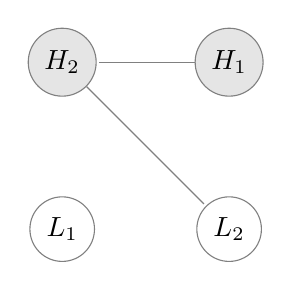
\begin{tikzpicture}[shorten >=1pt,draw=black!50]
	\node (H1) at ( 1.06,  1.06)	[circle, draw, fill = gray!20]	{$H_{1}$};
	\node (H2) at (-1.06,  1.06)	[circle, draw, fill = gray!20]	{$H_{2}$};
	\node (L1) at (-1.06, -1.06)	[circle, draw, fill = white]	{$L_{1}$};
	\node (L2) at ( 1.06, -1.06)	[circle, draw, fill = white]	{$L_{2}$};
	\draw (H1) -- (H2);
	\draw (H2) -- (L2);
\end{tikzpicture}
\end{center}
\columnbreak

\scaleeq{
Equations: \begin{cases}
	e^{H}_{1} \left(\frac{25 \phi}{3} - 3\right) = \alpha + 2 e^{H}_{2} - e^{L}_{1} \theta - 2 e^{L}_{2} \theta - \gamma\\
	e^{H}_{2} \left(\frac{25 \phi}{2} - 2\right) = \alpha + 3 e^{H}_{1} - e^{L}_{1} \theta + 3 e^{L}_{2} \theta - \gamma\\
	e^{L}_{1} \left(\frac{25 \phi}{4 \theta} - 4 \theta\right) = \alpha - 2 e^{H}_{1} - 3 e^{H}_{2} - 2 e^{L}_{2} \theta - \gamma\\
	e^{L}_{2} \left(\frac{25 \phi}{3 \theta} - 3 \theta\right) = \alpha - 2 e^{H}_{1} + 2 e^{H}_{2} - e^{L}_{1} \theta - \gamma
\end{cases}
}\end{multicols}


Optimal efforts:

\scaleeq{
\begin{cases}
	e^{H}_{1} &= \frac{15 \phi \left(\alpha - \gamma\right) \left(5 \phi - 4 \theta^{2}\right) \left(5 \phi - 3 \theta^{2}\right)}{3125 \phi^{4} - 3125 \phi^{3} \theta^{2} - 1625 \phi^{3} + 600 \phi^{2} \theta^{4} + 1025 \phi^{2} \theta^{2} + 180 \phi \theta^{2} - 72 \theta^{4}}\\
	e^{H}_{2} &= \frac{2 \left(\alpha - \gamma\right) \left(5 \phi - 3 \theta\right) \left(5 \phi + 3 \theta\right) \left(5 \phi - 4 \theta^{2}\right)}{3125 \phi^{4} - 3125 \phi^{3} \theta^{2} - 1625 \phi^{3} + 600 \phi^{2} \theta^{4} + 1025 \phi^{2} \theta^{2} + 180 \phi \theta^{2} - 72 \theta^{4}}\\
	e^{L}_{1} &= \frac{4 \theta \left(\alpha - \gamma\right) \left(125 \phi^{3} - 75 \phi^{2} \theta^{2} - 125 \phi^{2} + 45 \phi \theta^{2} + 18 \theta^{2}\right)}{3125 \phi^{4} - 3125 \phi^{3} \theta^{2} - 1625 \phi^{3} + 600 \phi^{2} \theta^{4} + 1025 \phi^{2} \theta^{2} + 180 \phi \theta^{2} - 72 \theta^{4}}\\
	e^{L}_{2} &= \frac{15 \phi \theta \left(\alpha - \gamma\right) \left(5 \phi - 3\right) \left(5 \phi - 4 \theta^{2}\right)}{3125 \phi^{4} - 3125 \phi^{3} \theta^{2} - 1625 \phi^{3} + 600 \phi^{2} \theta^{4} + 1025 \phi^{2} \theta^{2} + 180 \phi \theta^{2} - 72 \theta^{4}}
\end{cases}
}

Production Costs:

\scaleeq{
\begin{cases}
	c^{H}_{1} &= - \frac{625 \alpha \phi^{3} - 725 \alpha \phi^{2} \theta^{2} + 180 \alpha \phi \theta^{4} - 90 \alpha \phi \theta^{2} + 72 \alpha \theta^{4} - 3125 \gamma \phi^{4} + 3125 \gamma \phi^{3} \theta^{2} + 1000 \gamma \phi^{3} - 600 \gamma \phi^{2} \theta^{4} - 300 \gamma \phi^{2} \theta^{2} - 180 \gamma \phi \theta^{4} - 90 \gamma \phi \theta^{2}}{3125 \phi^{4} - 3125 \phi^{3} \theta^{2} - 1625 \phi^{3} + 600 \phi^{2} \theta^{4} + 1025 \phi^{2} \theta^{2} + 180 \phi \theta^{2} - 72 \theta^{4}}\\
	c^{H}_{2} &= - \frac{375 \alpha \phi^{3} \theta^{2} + 625 \alpha \phi^{3} - 300 \alpha \phi^{2} \theta^{4} - 950 \alpha \phi^{2} \theta^{2} + 360 \alpha \phi \theta^{4} - 90 \alpha \phi \theta^{2} + 72 \alpha \theta^{4} - 3125 \gamma \phi^{4} + 2750 \gamma \phi^{3} \theta^{2} + 1000 \gamma \phi^{3} - 300 \gamma \phi^{2} \theta^{4} - 75 \gamma \phi^{2} \theta^{2} - 360 \gamma \phi \theta^{4} - 90 \gamma \phi \theta^{2}}{3125 \phi^{4} - 3125 \phi^{3} \theta^{2} - 1625 \phi^{3} + 600 \phi^{2} \theta^{4} + 1025 \phi^{2} \theta^{2} + 180 \phi \theta^{2} - 72 \theta^{4}}\\
	c^{L}_{1} &= - \frac{500 \alpha \phi^{3} \theta^{2} - 300 \alpha \phi^{2} \theta^{4} - 500 \alpha \phi^{2} \theta^{2} + 180 \alpha \phi \theta^{4} + 72 \alpha \theta^{4} - 3125 \gamma \phi^{4} + 2625 \gamma \phi^{3} \theta^{2} + 1625 \gamma \phi^{3} - 300 \gamma \phi^{2} \theta^{4} - 525 \gamma \phi^{2} \theta^{2} - 180 \gamma \phi \theta^{4} - 180 \gamma \phi \theta^{2}}{3125 \phi^{4} - 3125 \phi^{3} \theta^{2} - 1625 \phi^{3} + 600 \phi^{2} \theta^{4} + 1025 \phi^{2} \theta^{2} + 180 \phi \theta^{2} - 72 \theta^{4}}\\
	c^{L}_{2} &= - \frac{375 \alpha \phi^{3} \theta^{2} + 250 \alpha \phi^{3} - 300 \alpha \phi^{2} \theta^{4} - 425 \alpha \phi^{2} \theta^{2} + 180 \alpha \phi \theta^{4} - 90 \alpha \phi \theta^{2} + 72 \alpha \theta^{4} - 3125 \gamma \phi^{4} + 2750 \gamma \phi^{3} \theta^{2} + 1375 \gamma \phi^{3} - 300 \gamma \phi^{2} \theta^{4} - 600 \gamma \phi^{2} \theta^{2} - 180 \gamma \phi \theta^{4} - 90 \gamma \phi \theta^{2}}{3125 \phi^{4} - 3125 \phi^{3} \theta^{2} - 1625 \phi^{3} + 600 \phi^{2} \theta^{4} + 1025 \phi^{2} \theta^{2} + 180 \phi \theta^{2} - 72 \theta^{4}}
\end{cases}
}

Production Quantities:

\scaleeq{
\begin{cases}
	q^{H}_{1} &= \frac{25 \phi^{2} \left(\alpha - \gamma\right) \left(5 \phi - 4 \theta^{2}\right) \left(5 \phi - 3 \theta^{2}\right)}{3125 \phi^{4} - 3125 \phi^{3} \theta^{2} - 1625 \phi^{3} + 600 \phi^{2} \theta^{4} + 1025 \phi^{2} \theta^{2} + 180 \phi \theta^{2} - 72 \theta^{4}}\\
	q^{H}_{2} &= \frac{5 \phi \left(\alpha - \gamma\right) \left(5 \phi - 3 \theta\right) \left(5 \phi + 3 \theta\right) \left(5 \phi - 4 \theta^{2}\right)}{3125 \phi^{4} - 3125 \phi^{3} \theta^{2} - 1625 \phi^{3} + 600 \phi^{2} \theta^{4} + 1025 \phi^{2} \theta^{2} + 180 \phi \theta^{2} - 72 \theta^{4}}\\
	q^{L}_{1} &= \frac{5 \phi \left(\alpha - \gamma\right) \left(125 \phi^{3} - 75 \phi^{2} \theta^{2} - 125 \phi^{2} + 45 \phi \theta^{2} + 18 \theta^{2}\right)}{3125 \phi^{4} - 3125 \phi^{3} \theta^{2} - 1625 \phi^{3} + 600 \phi^{2} \theta^{4} + 1025 \phi^{2} \theta^{2} + 180 \phi \theta^{2} - 72 \theta^{4}}\\
	q^{L}_{2} &= \frac{25 \phi^{2} \left(\alpha - \gamma\right) \left(5 \phi - 3\right) \left(5 \phi - 4 \theta^{2}\right)}{3125 \phi^{4} - 3125 \phi^{3} \theta^{2} - 1625 \phi^{3} + 600 \phi^{2} \theta^{4} + 1025 \phi^{2} \theta^{2} + 180 \phi \theta^{2} - 72 \theta^{4}}
\end{cases}
}

Profits:

\begin{equation}
\label{eq:E2A:2H2L_profit}
\scaledequation{\begin{cases}
	\pi^{H}_{1} &= \frac{25 \phi^{3} \left(\alpha - \gamma\right)^{2} \left(5 \phi - 4 \theta^{2}\right)^{2} \left(5 \phi - 3 \theta^{2}\right)^{2} \left(25 \phi - 9\right)}{\left(3125 \phi^{4} - 3125 \phi^{3} \theta^{2} - 1625 \phi^{3} + 600 \phi^{2} \theta^{4} + 1025 \phi^{2} \theta^{2} + 180 \phi \theta^{2} - 72 \theta^{4}\right)^{2}}\\
	\pi^{H}_{2} &= \frac{\phi \left(\alpha - \gamma\right)^{2} \left(5 \phi - 3 \theta\right)^{2} \left(5 \phi + 3 \theta\right)^{2} \left(5 \phi - 4 \theta^{2}\right)^{2} \left(25 \phi - 4\right)}{\left(3125 \phi^{4} - 3125 \phi^{3} \theta^{2} - 1625 \phi^{3} + 600 \phi^{2} \theta^{4} + 1025 \phi^{2} \theta^{2} + 180 \phi \theta^{2} - 72 \theta^{4}\right)^{2}}\\
	\pi^{L}_{1} &= \frac{\phi \left(\alpha - \gamma\right)^{2} \left(25 \phi - 16 \theta^{2}\right) \left(125 \phi^{3} - 75 \phi^{2} \theta^{2} - 125 \phi^{2} + 45 \phi \theta^{2} + 18 \theta^{2}\right)^{2}}{\left(3125 \phi^{4} - 3125 \phi^{3} \theta^{2} - 1625 \phi^{3} + 600 \phi^{2} \theta^{4} + 1025 \phi^{2} \theta^{2} + 180 \phi \theta^{2} - 72 \theta^{4}\right)^{2}}\\
	\pi^{L}_{2} &= \frac{25 \phi^{3} \left(\alpha - \gamma\right)^{2} \left(5 \phi - 3\right)^{2} \left(5 \phi - 4 \theta^{2}\right)^{2} \left(25 \phi - 9 \theta^{2}\right)}{\left(3125 \phi^{4} - 3125 \phi^{3} \theta^{2} - 1625 \phi^{3} + 600 \phi^{2} \theta^{4} + 1025 \phi^{2} \theta^{2} + 180 \phi \theta^{2} - 72 \theta^{4}\right)^{2}}
\end{cases}
}
\end{equation}

Total Production:

\scaleeq{
\frac{10 \phi \left(\alpha - \gamma\right) \left(250 \phi^{3} - 225 \phi^{2} \theta^{2} - 100 \phi^{2} + 30 \phi \theta^{4} + 30 \phi \theta^{2} + 18 \theta^{4} + 9 \theta^{2}\right)}{3125 \phi^{4} - 3125 \phi^{3} \theta^{2} - 1625 \phi^{3} + 600 \phi^{2} \theta^{4} + 1025 \phi^{2} \theta^{2} + 180 \phi \theta^{2} - 72 \theta^{4}}
}

Price:

\scaleeq{
\frac{625 \alpha \phi^{4} - 875 \alpha \phi^{3} \theta^{2} - 625 \alpha \phi^{3} + 300 \alpha \phi^{2} \theta^{4} + 725 \alpha \phi^{2} \theta^{2} - 180 \alpha \phi \theta^{4} + 90 \alpha \phi \theta^{2} - 72 \alpha \theta^{4} + 2500 \gamma \phi^{4} - 2250 \gamma \phi^{3} \theta^{2} - 1000 \gamma \phi^{3} + 300 \gamma \phi^{2} \theta^{4} + 300 \gamma \phi^{2} \theta^{2} + 180 \gamma \phi \theta^{4} + 90 \gamma \phi \theta^{2}}{3125 \phi^{4} - 3125 \phi^{3} \theta^{2} - 1625 \phi^{3} + 600 \phi^{2} \theta^{4} + 1025 \phi^{2} \theta^{2} + 180 \phi \theta^{2} - 72 \theta^{4}}
}

Firm Surplus:

\scaleeq{
\frac{\phi \left(\alpha - \gamma\right)^{2} \left(1562500 \phi^{7} - 3203125 \phi^{6} \theta^{2} - 1453125 \phi^{6} + 2306250 \phi^{5} \theta^{4} + 2381250 \phi^{5} \theta^{2} + 531250 \phi^{5} - 705000 \phi^{4} \theta^{6} - 1219375 \phi^{4} \theta^{4} - 649375 \phi^{4} \theta^{2} + 90000 \phi^{3} \theta^{8} + 225000 \phi^{3} \theta^{6} + 240750 \phi^{3} \theta^{4} - 112500 \phi^{3} \theta^{2} - 32400 \phi^{2} \theta^{8} - 73800 \phi^{2} \theta^{6} + 104400 \phi^{2} \theta^{4} + 32400 \phi \theta^{8} - 12960 \phi \theta^{6} + 8100 \phi \theta^{4} - 5184 \theta^{8} - 5184 \theta^{6}\right)}{\left(3125 \phi^{4} - 3125 \phi^{3} \theta^{2} - 1625 \phi^{3} + 600 \phi^{2} \theta^{4} + 1025 \phi^{2} \theta^{2} + 180 \phi \theta^{2} - 72 \theta^{4}\right)^{2}}
}

Consumer Surplus:

\scaleeq{
\frac{50 \phi^{2} \left(\alpha - \gamma\right)^{2} \left(250 \phi^{3} - 225 \phi^{2} \theta^{2} - 100 \phi^{2} + 30 \phi \theta^{4} + 30 \phi \theta^{2} + 18 \theta^{4} + 9 \theta^{2}\right)^{2}}{\left(3125 \phi^{4} - 3125 \phi^{3} \theta^{2} - 1625 \phi^{3} + 600 \phi^{2} \theta^{4} + 1025 \phi^{2} \theta^{2} + 180 \phi \theta^{2} - 72 \theta^{4}\right)^{2}}
}

Social Welfare:

\scaleeq{
\frac{\phi \left(\alpha - \gamma\right)^{2} \left(4687500 \phi^{7} - 8828125 \phi^{6} \theta^{2} - 3953125 \phi^{6} + 5587500 \phi^{5} \theta^{4} + 5381250 \phi^{5} \theta^{2} + 1031250 \phi^{5} - 1380000 \phi^{4} \theta^{6} - 1744375 \phi^{4} \theta^{4} - 724375 \phi^{4} \theta^{2} + 135000 \phi^{3} \theta^{8} - 90000 \phi^{3} \theta^{6} - 96750 \phi^{3} \theta^{4} - 202500 \phi^{3} \theta^{2} + 21600 \phi^{2} \theta^{8} + 7200 \phi^{2} \theta^{6} + 131400 \phi^{2} \theta^{4} + 48600 \phi \theta^{8} + 3240 \phi \theta^{6} + 12150 \phi \theta^{4} - 5184 \theta^{8} - 5184 \theta^{6}\right)}{\left(3125 \phi^{4} - 3125 \phi^{3} \theta^{2} - 1625 \phi^{3} + 600 \phi^{2} \theta^{4} + 1025 \phi^{2} \theta^{2} + 180 \phi \theta^{2} - 72 \theta^{4}\right)^{2}}
}

%======================================================================

\subsubsection{E2B [2H2L]}
\label{apx:E2B:2H2L}

\begin{multicols}{2}
\begin{center}
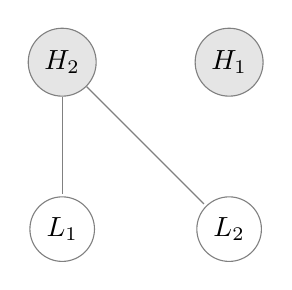
\begin{tikzpicture}[shorten >=1pt,draw=black!50]
	\node (H1) at ( 1.06,  1.06)	[circle, draw, fill = gray!20]	{$H_{1}$};
	\node (H2) at (-1.06,  1.06)	[circle, draw, fill = gray!20]	{$H_{2}$};
	\node (L1) at (-1.06, -1.06)	[circle, draw, fill = white]	{$L_{1}$};
	\node (L2) at ( 1.06, -1.06)	[circle, draw, fill = white]	{$L_{2}$};
	\draw (H2) -- (L1);
	\draw (H2) -- (L2);
\end{tikzpicture}
\end{center}
\columnbreak

\scaleeq{
Equations: \begin{cases}
	e^{H}_{1} \left(\frac{25 \phi}{4} - 4\right) = \alpha - 3 e^{H}_{2} - 2 e^{L}_{1} \theta - 2 e^{L}_{2} \theta - \gamma\\
	e^{H}_{2} \left(\frac{25 \phi}{2} - 2\right) = \alpha - e^{H}_{1} + 3 e^{L}_{1} \theta + 3 e^{L}_{2} \theta - \gamma\\
	e^{L}_{1} \left(\frac{25 \phi}{3 \theta} - 3 \theta\right) = \alpha - e^{H}_{1} + 2 e^{H}_{2} - 2 e^{L}_{2} \theta - \gamma\\
	e^{L}_{2} \left(\frac{25 \phi}{3 \theta} - 3 \theta\right) = \alpha - e^{H}_{1} + 2 e^{H}_{2} - 2 e^{L}_{1} \theta - \gamma
\end{cases}
}\end{multicols}


Optimal efforts:

\scaleeq{
\begin{cases}
	e^{H}_{1} &= \frac{4 \left(\alpha - \gamma\right) \left(25 \phi^{2} - 15 \phi \theta^{2} - 10 \phi - 6 \theta^{2}\right)}{625 \phi^{3} - 75 \phi^{2} \theta^{2} - 500 \phi^{2} - 60 \phi \theta^{2} + 40 \phi + 24 \theta^{2}}\\
	e^{H}_{2} &= \frac{2 \left(\alpha - \gamma\right) \left(5 \phi - 4\right) \left(5 \phi + 3 \theta^{2}\right)}{625 \phi^{3} - 75 \phi^{2} \theta^{2} - 500 \phi^{2} - 60 \phi \theta^{2} + 40 \phi + 24 \theta^{2}}\\
	e^{L}_{1} &= \frac{15 \phi \theta \left(\alpha - \gamma\right) \left(5 \phi - 4\right)}{625 \phi^{3} - 75 \phi^{2} \theta^{2} - 500 \phi^{2} - 60 \phi \theta^{2} + 40 \phi + 24 \theta^{2}}\\
	e^{L}_{2} &= \frac{15 \phi \theta \left(\alpha - \gamma\right) \left(5 \phi - 4\right)}{625 \phi^{3} - 75 \phi^{2} \theta^{2} - 500 \phi^{2} - 60 \phi \theta^{2} + 40 \phi + 24 \theta^{2}}
\end{cases}
}

Production Costs:

\scaleeq{
\begin{cases}
	c^{H}_{1} &= - \frac{100 \alpha \phi^{2} - 60 \alpha \phi \theta^{2} - 40 \alpha \phi - 24 \alpha \theta^{2} - 625 \gamma \phi^{3} + 75 \gamma \phi^{2} \theta^{2} + 400 \gamma \phi^{2} + 120 \gamma \phi \theta^{2}}{625 \phi^{3} - 75 \phi^{2} \theta^{2} - 500 \phi^{2} - 60 \phi \theta^{2} + 40 \phi + 24 \theta^{2}}\\
	c^{H}_{2} &= - \frac{150 \alpha \phi^{2} \theta^{2} + 50 \alpha \phi^{2} - 90 \alpha \phi \theta^{2} - 40 \alpha \phi - 24 \alpha \theta^{2} - 625 \gamma \phi^{3} - 75 \gamma \phi^{2} \theta^{2} + 450 \gamma \phi^{2} + 150 \gamma \phi \theta^{2}}{625 \phi^{3} - 75 \phi^{2} \theta^{2} - 500 \phi^{2} - 60 \phi \theta^{2} + 40 \phi + 24 \theta^{2}}\\
	c^{L}_{1} &= - \frac{75 \alpha \phi^{2} \theta^{2} + 50 \alpha \phi^{2} - 30 \alpha \phi \theta^{2} - 40 \alpha \phi - 24 \alpha \theta^{2} - 625 \gamma \phi^{3} + 450 \gamma \phi^{2} + 90 \gamma \phi \theta^{2}}{625 \phi^{3} - 75 \phi^{2} \theta^{2} - 500 \phi^{2} - 60 \phi \theta^{2} + 40 \phi + 24 \theta^{2}}\\
	c^{L}_{2} &= - \frac{75 \alpha \phi^{2} \theta^{2} + 50 \alpha \phi^{2} - 30 \alpha \phi \theta^{2} - 40 \alpha \phi - 24 \alpha \theta^{2} - 625 \gamma \phi^{3} + 450 \gamma \phi^{2} + 90 \gamma \phi \theta^{2}}{625 \phi^{3} - 75 \phi^{2} \theta^{2} - 500 \phi^{2} - 60 \phi \theta^{2} + 40 \phi + 24 \theta^{2}}
\end{cases}
}

Production Quantities:

\scaleeq{
\begin{cases}
	q^{H}_{1} &= \frac{5 \phi \left(\alpha - \gamma\right) \left(25 \phi^{2} - 15 \phi \theta^{2} - 10 \phi - 6 \theta^{2}\right)}{625 \phi^{3} - 75 \phi^{2} \theta^{2} - 500 \phi^{2} - 60 \phi \theta^{2} + 40 \phi + 24 \theta^{2}}\\
	q^{H}_{2} &= \frac{5 \phi \left(\alpha - \gamma\right) \left(5 \phi - 4\right) \left(5 \phi + 3 \theta^{2}\right)}{625 \phi^{3} - 75 \phi^{2} \theta^{2} - 500 \phi^{2} - 60 \phi \theta^{2} + 40 \phi + 24 \theta^{2}}\\
	q^{L}_{1} &= \frac{25 \phi^{2} \left(\alpha - \gamma\right) \left(5 \phi - 4\right)}{625 \phi^{3} - 75 \phi^{2} \theta^{2} - 500 \phi^{2} - 60 \phi \theta^{2} + 40 \phi + 24 \theta^{2}}\\
	q^{L}_{2} &= \frac{25 \phi^{2} \left(\alpha - \gamma\right) \left(5 \phi - 4\right)}{625 \phi^{3} - 75 \phi^{2} \theta^{2} - 500 \phi^{2} - 60 \phi \theta^{2} + 40 \phi + 24 \theta^{2}}
\end{cases}
}

Profits:

\begin{equation}
\label{eq:E2B:2H2L_profit}
\scaledequation{\begin{cases}
	\pi^{H}_{1} &= \frac{\phi \left(\alpha - \gamma\right)^{2} \left(25 \phi - 16\right) \left(25 \phi^{2} - 15 \phi \theta^{2} - 10 \phi - 6 \theta^{2}\right)^{2}}{\left(625 \phi^{3} - 75 \phi^{2} \theta^{2} - 500 \phi^{2} - 60 \phi \theta^{2} + 40 \phi + 24 \theta^{2}\right)^{2}}\\
	\pi^{H}_{2} &= \frac{\phi \left(\alpha - \gamma\right)^{2} \left(5 \phi - 4\right)^{2} \left(5 \phi + 3 \theta^{2}\right)^{2} \left(25 \phi - 4\right)}{\left(625 \phi^{3} - 75 \phi^{2} \theta^{2} - 500 \phi^{2} - 60 \phi \theta^{2} + 40 \phi + 24 \theta^{2}\right)^{2}}\\
	\pi^{L}_{1} &= \frac{25 \phi^{3} \left(\alpha - \gamma\right)^{2} \left(5 \phi - 4\right)^{2} \left(25 \phi - 9 \theta^{2}\right)}{\left(625 \phi^{3} - 75 \phi^{2} \theta^{2} - 500 \phi^{2} - 60 \phi \theta^{2} + 40 \phi + 24 \theta^{2}\right)^{2}}\\
	\pi^{L}_{2} &= \frac{25 \phi^{3} \left(\alpha - \gamma\right)^{2} \left(5 \phi - 4\right)^{2} \left(25 \phi - 9 \theta^{2}\right)}{\left(625 \phi^{3} - 75 \phi^{2} \theta^{2} - 500 \phi^{2} - 60 \phi \theta^{2} + 40 \phi + 24 \theta^{2}\right)^{2}}
\end{cases}
}
\end{equation}

Total Production:

\scaleeq{
\frac{10 \phi \left(\alpha - \gamma\right) \left(50 \phi^{2} - 35 \phi - 9 \theta^{2}\right)}{625 \phi^{3} - 75 \phi^{2} \theta^{2} - 500 \phi^{2} - 60 \phi \theta^{2} + 40 \phi + 24 \theta^{2}}
}

Price:

\scaleeq{
\frac{125 \alpha \phi^{3} - 75 \alpha \phi^{2} \theta^{2} - 150 \alpha \phi^{2} + 30 \alpha \phi \theta^{2} + 40 \alpha \phi + 24 \alpha \theta^{2} + 500 \gamma \phi^{3} - 350 \gamma \phi^{2} - 90 \gamma \phi \theta^{2}}{625 \phi^{3} - 75 \phi^{2} \theta^{2} - 500 \phi^{2} - 60 \phi \theta^{2} + 40 \phi + 24 \theta^{2}}
}

Firm Surplus:

\scaleeq{
\frac{2 \phi \left(\alpha - \gamma\right)^{2} \left(31250 \phi^{5} - 5625 \phi^{4} \theta^{2} - 50000 \phi^{4} + 5625 \phi^{3} \theta^{4} - 1500 \phi^{3} \theta^{2} + 22250 \phi^{3} - 4500 \phi^{2} \theta^{4} + 6300 \phi^{2} \theta^{2} - 1600 \phi^{2} + 1530 \phi \theta^{4} - 1920 \phi \theta^{2} - 576 \theta^{4}\right)}{\left(625 \phi^{3} - 75 \phi^{2} \theta^{2} - 500 \phi^{2} - 60 \phi \theta^{2} + 40 \phi + 24 \theta^{2}\right)^{2}}
}

Consumer Surplus:

\scaleeq{
\frac{50 \phi^{2} \left(\alpha - \gamma\right)^{2} \left(50 \phi^{2} - 35 \phi - 9 \theta^{2}\right)^{2}}{\left(625 \phi^{3} - 75 \phi^{2} \theta^{2} - 500 \phi^{2} - 60 \phi \theta^{2} + 40 \phi + 24 \theta^{2}\right)^{2}}
}

Social Welfare:

\scaleeq{
\frac{2 \phi \left(\alpha - \gamma\right)^{2} \left(93750 \phi^{5} - 5625 \phi^{4} \theta^{2} - 137500 \phi^{4} + 5625 \phi^{3} \theta^{4} - 24000 \phi^{3} \theta^{2} + 52875 \phi^{3} - 4500 \phi^{2} \theta^{4} + 22050 \phi^{2} \theta^{2} - 1600 \phi^{2} + 3555 \phi \theta^{4} - 1920 \phi \theta^{2} - 576 \theta^{4}\right)}{\left(625 \phi^{3} - 75 \phi^{2} \theta^{2} - 500 \phi^{2} - 60 \phi \theta^{2} + 40 \phi + 24 \theta^{2}\right)^{2}}
}

%======================================================================

\subsubsection{E2C [2H2L]}
\label{apx:E2C:2H2L}

\begin{multicols}{2}
\begin{center}
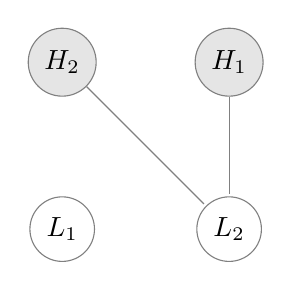
\begin{tikzpicture}[shorten >=1pt,draw=black!50]
	\node (H1) at ( 1.06,  1.06)	[circle, draw, fill = gray!20]	{$H_{1}$};
	\node (H2) at (-1.06,  1.06)	[circle, draw, fill = gray!20]	{$H_{2}$};
	\node (L1) at (-1.06, -1.06)	[circle, draw, fill = white]	{$L_{1}$};
	\node (L2) at ( 1.06, -1.06)	[circle, draw, fill = white]	{$L_{2}$};
	\draw (H1) -- (L2);
	\draw (H2) -- (L2);
\end{tikzpicture}
\end{center}
\columnbreak

\scaleeq{
Equations: \begin{cases}
	e^{H}_{1} \left(\frac{25 \phi}{3} - 3\right) = \alpha - 2 e^{H}_{2} - e^{L}_{1} \theta + 2 e^{L}_{2} \theta - \gamma\\
	e^{H}_{2} \left(\frac{25 \phi}{3} - 3\right) = \alpha - 2 e^{H}_{1} - e^{L}_{1} \theta + 2 e^{L}_{2} \theta - \gamma\\
	e^{L}_{1} \left(\frac{25 \phi}{4 \theta} - 4 \theta\right) = \alpha - 2 e^{H}_{1} - 2 e^{H}_{2} - 3 e^{L}_{2} \theta - \gamma\\
	e^{L}_{2} \left(\frac{25 \phi}{2 \theta} - 2 \theta\right) = \alpha + 3 e^{H}_{1} + 3 e^{H}_{2} - e^{L}_{1} \theta - \gamma
\end{cases}
}\end{multicols}


Optimal efforts:

\scaleeq{
\begin{cases}
	e^{H}_{1} &= \frac{15 \phi \left(\alpha - \gamma\right) \left(5 \phi - 4 \theta^{2}\right)}{625 \phi^{3} - 500 \phi^{2} \theta^{2} - 75 \phi^{2} + 40 \phi \theta^{4} - 60 \phi \theta^{2} + 24 \theta^{4}}\\
	e^{H}_{2} &= \frac{15 \phi \left(\alpha - \gamma\right) \left(5 \phi - 4 \theta^{2}\right)}{625 \phi^{3} - 500 \phi^{2} \theta^{2} - 75 \phi^{2} + 40 \phi \theta^{4} - 60 \phi \theta^{2} + 24 \theta^{4}}\\
	e^{L}_{1} &= \frac{4 \theta \left(\alpha - \gamma\right) \left(25 \phi^{2} - 10 \phi \theta^{2} - 15 \phi - 6 \theta^{2}\right)}{625 \phi^{3} - 500 \phi^{2} \theta^{2} - 75 \phi^{2} + 40 \phi \theta^{4} - 60 \phi \theta^{2} + 24 \theta^{4}}\\
	e^{L}_{2} &= \frac{2 \theta \left(\alpha - \gamma\right) \left(5 \phi + 3\right) \left(5 \phi - 4 \theta^{2}\right)}{625 \phi^{3} - 500 \phi^{2} \theta^{2} - 75 \phi^{2} + 40 \phi \theta^{4} - 60 \phi \theta^{2} + 24 \theta^{4}}
\end{cases}
}

Production Costs:

\scaleeq{
\begin{cases}
	c^{H}_{1} &= - \frac{50 \alpha \phi^{2} \theta^{2} + 75 \alpha \phi^{2} - 40 \alpha \phi \theta^{4} - 30 \alpha \phi \theta^{2} - 24 \alpha \theta^{4} - 625 \gamma \phi^{3} + 450 \gamma \phi^{2} \theta^{2} + 90 \gamma \phi \theta^{2}}{625 \phi^{3} - 500 \phi^{2} \theta^{2} - 75 \phi^{2} + 40 \phi \theta^{4} - 60 \phi \theta^{2} + 24 \theta^{4}}\\
	c^{H}_{2} &= - \frac{50 \alpha \phi^{2} \theta^{2} + 75 \alpha \phi^{2} - 40 \alpha \phi \theta^{4} - 30 \alpha \phi \theta^{2} - 24 \alpha \theta^{4} - 625 \gamma \phi^{3} + 450 \gamma \phi^{2} \theta^{2} + 90 \gamma \phi \theta^{2}}{625 \phi^{3} - 500 \phi^{2} \theta^{2} - 75 \phi^{2} + 40 \phi \theta^{4} - 60 \phi \theta^{2} + 24 \theta^{4}}\\
	c^{L}_{1} &= - \frac{100 \alpha \phi^{2} \theta^{2} - 40 \alpha \phi \theta^{4} - 60 \alpha \phi \theta^{2} - 24 \alpha \theta^{4} - 625 \gamma \phi^{3} + 400 \gamma \phi^{2} \theta^{2} + 75 \gamma \phi^{2} + 120 \gamma \phi \theta^{2}}{625 \phi^{3} - 500 \phi^{2} \theta^{2} - 75 \phi^{2} + 40 \phi \theta^{4} - 60 \phi \theta^{2} + 24 \theta^{4}}\\
	c^{L}_{2} &= - \frac{50 \alpha \phi^{2} \theta^{2} + 150 \alpha \phi^{2} - 40 \alpha \phi \theta^{4} - 90 \alpha \phi \theta^{2} - 24 \alpha \theta^{4} - 625 \gamma \phi^{3} + 450 \gamma \phi^{2} \theta^{2} - 75 \gamma \phi^{2} + 150 \gamma \phi \theta^{2}}{625 \phi^{3} - 500 \phi^{2} \theta^{2} - 75 \phi^{2} + 40 \phi \theta^{4} - 60 \phi \theta^{2} + 24 \theta^{4}}
\end{cases}
}

Production Quantities:

\scaleeq{
\begin{cases}
	q^{H}_{1} &= \frac{25 \phi^{2} \left(\alpha - \gamma\right) \left(5 \phi - 4 \theta^{2}\right)}{625 \phi^{3} - 500 \phi^{2} \theta^{2} - 75 \phi^{2} + 40 \phi \theta^{4} - 60 \phi \theta^{2} + 24 \theta^{4}}\\
	q^{H}_{2} &= \frac{25 \phi^{2} \left(\alpha - \gamma\right) \left(5 \phi - 4 \theta^{2}\right)}{625 \phi^{3} - 500 \phi^{2} \theta^{2} - 75 \phi^{2} + 40 \phi \theta^{4} - 60 \phi \theta^{2} + 24 \theta^{4}}\\
	q^{L}_{1} &= \frac{5 \phi \left(\alpha - \gamma\right) \left(25 \phi^{2} - 10 \phi \theta^{2} - 15 \phi - 6 \theta^{2}\right)}{625 \phi^{3} - 500 \phi^{2} \theta^{2} - 75 \phi^{2} + 40 \phi \theta^{4} - 60 \phi \theta^{2} + 24 \theta^{4}}\\
	q^{L}_{2} &= \frac{5 \phi \left(\alpha - \gamma\right) \left(5 \phi + 3\right) \left(5 \phi - 4 \theta^{2}\right)}{625 \phi^{3} - 500 \phi^{2} \theta^{2} - 75 \phi^{2} + 40 \phi \theta^{4} - 60 \phi \theta^{2} + 24 \theta^{4}}
\end{cases}
}

Profits:

\begin{equation}
\label{eq:E2C:2H2L_profit}
\scaledequation{\begin{cases}
	\pi^{H}_{1} &= \frac{25 \phi^{3} \left(\alpha - \gamma\right)^{2} \left(5 \phi - 4 \theta^{2}\right)^{2} \left(25 \phi - 9\right)}{\left(625 \phi^{3} - 500 \phi^{2} \theta^{2} - 75 \phi^{2} + 40 \phi \theta^{4} - 60 \phi \theta^{2} + 24 \theta^{4}\right)^{2}}\\
	\pi^{H}_{2} &= \frac{25 \phi^{3} \left(\alpha - \gamma\right)^{2} \left(5 \phi - 4 \theta^{2}\right)^{2} \left(25 \phi - 9\right)}{\left(625 \phi^{3} - 500 \phi^{2} \theta^{2} - 75 \phi^{2} + 40 \phi \theta^{4} - 60 \phi \theta^{2} + 24 \theta^{4}\right)^{2}}\\
	\pi^{L}_{1} &= \frac{\phi \left(\alpha - \gamma\right)^{2} \left(25 \phi - 16 \theta^{2}\right) \left(25 \phi^{2} - 10 \phi \theta^{2} - 15 \phi - 6 \theta^{2}\right)^{2}}{\left(625 \phi^{3} - 500 \phi^{2} \theta^{2} - 75 \phi^{2} + 40 \phi \theta^{4} - 60 \phi \theta^{2} + 24 \theta^{4}\right)^{2}}\\
	\pi^{L}_{2} &= \frac{\phi \left(\alpha - \gamma\right)^{2} \left(5 \phi + 3\right)^{2} \left(5 \phi - 4 \theta^{2}\right)^{2} \left(25 \phi - 4 \theta^{2}\right)}{\left(625 \phi^{3} - 500 \phi^{2} \theta^{2} - 75 \phi^{2} + 40 \phi \theta^{4} - 60 \phi \theta^{2} + 24 \theta^{4}\right)^{2}}
\end{cases}
}
\end{equation}

Total Production:

\scaleeq{
\frac{10 \phi \left(\alpha - \gamma\right) \left(50 \phi^{2} - 35 \phi \theta^{2} - 9 \theta^{2}\right)}{625 \phi^{3} - 500 \phi^{2} \theta^{2} - 75 \phi^{2} + 40 \phi \theta^{4} - 60 \phi \theta^{2} + 24 \theta^{4}}
}

Price:

\scaleeq{
\frac{125 \alpha \phi^{3} - 150 \alpha \phi^{2} \theta^{2} - 75 \alpha \phi^{2} + 40 \alpha \phi \theta^{4} + 30 \alpha \phi \theta^{2} + 24 \alpha \theta^{4} + 500 \gamma \phi^{3} - 350 \gamma \phi^{2} \theta^{2} - 90 \gamma \phi \theta^{2}}{625 \phi^{3} - 500 \phi^{2} \theta^{2} - 75 \phi^{2} + 40 \phi \theta^{4} - 60 \phi \theta^{2} + 24 \theta^{4}}
}

Firm Surplus:

\scaleeq{
\frac{2 \phi \left(\alpha - \gamma\right)^{2} \left(31250 \phi^{5} - 50000 \phi^{4} \theta^{2} - 5625 \phi^{4} + 22250 \phi^{3} \theta^{4} - 1500 \phi^{3} \theta^{2} + 5625 \phi^{3} - 1600 \phi^{2} \theta^{6} + 6300 \phi^{2} \theta^{4} - 4500 \phi^{2} \theta^{2} - 1920 \phi \theta^{6} + 1530 \phi \theta^{4} - 576 \theta^{6}\right)}{\left(625 \phi^{3} - 500 \phi^{2} \theta^{2} - 75 \phi^{2} + 40 \phi \theta^{4} - 60 \phi \theta^{2} + 24 \theta^{4}\right)^{2}}
}

Consumer Surplus:

\scaleeq{
\frac{50 \phi^{2} \left(\alpha - \gamma\right)^{2} \left(50 \phi^{2} - 35 \phi \theta^{2} - 9 \theta^{2}\right)^{2}}{\left(625 \phi^{3} - 500 \phi^{2} \theta^{2} - 75 \phi^{2} + 40 \phi \theta^{4} - 60 \phi \theta^{2} + 24 \theta^{4}\right)^{2}}
}

Social Welfare:

\scaleeq{
\frac{2 \phi \left(\alpha - \gamma\right)^{2} \left(93750 \phi^{5} - 137500 \phi^{4} \theta^{2} - 5625 \phi^{4} + 52875 \phi^{3} \theta^{4} - 24000 \phi^{3} \theta^{2} + 5625 \phi^{3} - 1600 \phi^{2} \theta^{6} + 22050 \phi^{2} \theta^{4} - 4500 \phi^{2} \theta^{2} - 1920 \phi \theta^{6} + 3555 \phi \theta^{4} - 576 \theta^{6}\right)}{\left(625 \phi^{3} - 500 \phi^{2} \theta^{2} - 75 \phi^{2} + 40 \phi \theta^{4} - 60 \phi \theta^{2} + 24 \theta^{4}\right)^{2}}
}

%======================================================================

\subsubsection{E2D [2H2L]}
\label{apx:E2D:2H2L}

\begin{multicols}{2}
\begin{center}
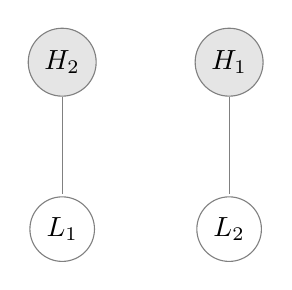
\begin{tikzpicture}[shorten >=1pt,draw=black!50]
	\node (H1) at ( 1.06,  1.06)	[circle, draw, fill = gray!20]	{$H_{1}$};
	\node (H2) at (-1.06,  1.06)	[circle, draw, fill = gray!20]	{$H_{2}$};
	\node (L1) at (-1.06, -1.06)	[circle, draw, fill = white]	{$L_{1}$};
	\node (L2) at ( 1.06, -1.06)	[circle, draw, fill = white]	{$L_{2}$};
	\draw (H1) -- (L2);
	\draw (H2) -- (L1);
\end{tikzpicture}
\end{center}
\columnbreak

\scaleeq{
Equations: \begin{cases}
	e^{H}_{1} \left(\frac{25 \phi}{3} - 3\right) = \alpha - 2 e^{H}_{2} - 2 e^{L}_{1} \theta + 3 e^{L}_{2} \theta - \gamma\\
	e^{H}_{2} \left(\frac{25 \phi}{3} - 3\right) = \alpha - 2 e^{H}_{1} + 3 e^{L}_{1} \theta - 2 e^{L}_{2} \theta - \gamma\\
	e^{L}_{1} \left(\frac{25 \phi}{3 \theta} - 3 \theta\right) = \alpha - 2 e^{H}_{1} + 3 e^{H}_{2} - 2 e^{L}_{2} \theta - \gamma\\
	e^{L}_{2} \left(\frac{25 \phi}{3 \theta} - 3 \theta\right) = \alpha + 3 e^{H}_{1} - 2 e^{H}_{2} - 2 e^{L}_{1} \theta - \gamma
\end{cases}
}\end{multicols}


Optimal efforts:

\scaleeq{
\begin{cases}
	e^{H}_{1} &= \frac{3 \left(\alpha - \gamma\right)}{25 \phi - 3 \theta^{2} - 3}\\
	e^{H}_{2} &= \frac{3 \left(\alpha - \gamma\right)}{25 \phi - 3 \theta^{2} - 3}\\
	e^{L}_{1} &= \frac{3 \theta \left(\alpha - \gamma\right)}{25 \phi - 3 \theta^{2} - 3}\\
	e^{L}_{2} &= \frac{3 \theta \left(\alpha - \gamma\right)}{25 \phi - 3 \theta^{2} - 3}
\end{cases}
}

Production Costs:

\scaleeq{
\begin{cases}
	c^{H}_{1} &= - \frac{3 \alpha \theta^{2} + 3 \alpha - 25 \gamma \phi}{25 \phi - 3 \theta^{2} - 3}\\
	c^{H}_{2} &= - \frac{3 \alpha \theta^{2} + 3 \alpha - 25 \gamma \phi}{25 \phi - 3 \theta^{2} - 3}\\
	c^{L}_{1} &= - \frac{3 \alpha \theta^{2} + 3 \alpha - 25 \gamma \phi}{25 \phi - 3 \theta^{2} - 3}\\
	c^{L}_{2} &= - \frac{3 \alpha \theta^{2} + 3 \alpha - 25 \gamma \phi}{25 \phi - 3 \theta^{2} - 3}
\end{cases}
}

Production Quantities:

\scaleeq{
\begin{cases}
	q^{H}_{1} &= \frac{5 \phi \left(\alpha - \gamma\right)}{25 \phi - 3 \theta^{2} - 3}\\
	q^{H}_{2} &= \frac{5 \phi \left(\alpha - \gamma\right)}{25 \phi - 3 \theta^{2} - 3}\\
	q^{L}_{1} &= \frac{5 \phi \left(\alpha - \gamma\right)}{25 \phi - 3 \theta^{2} - 3}\\
	q^{L}_{2} &= \frac{5 \phi \left(\alpha - \gamma\right)}{25 \phi - 3 \theta^{2} - 3}
\end{cases}
}

Profits:

\begin{equation}
\label{eq:E2D:2H2L_profit}
\scaledequation{\begin{cases}
	\pi^{H}_{1} &= \frac{\phi \left(\alpha - \gamma\right)^{2} \left(25 \phi - 9\right)}{\left(25 \phi - 3 \theta^{2} - 3\right)^{2}}\\
	\pi^{H}_{2} &= \frac{\phi \left(\alpha - \gamma\right)^{2} \left(25 \phi - 9\right)}{\left(25 \phi - 3 \theta^{2} - 3\right)^{2}}\\
	\pi^{L}_{1} &= \frac{\phi \left(\alpha - \gamma\right)^{2} \left(25 \phi - 9 \theta^{2}\right)}{\left(25 \phi - 3 \theta^{2} - 3\right)^{2}}\\
	\pi^{L}_{2} &= \frac{\phi \left(\alpha - \gamma\right)^{2} \left(25 \phi - 9 \theta^{2}\right)}{\left(25 \phi - 3 \theta^{2} - 3\right)^{2}}
\end{cases}
}
\end{equation}

Total Production:

\scaleeq{
\frac{20 \phi \left(\alpha - \gamma\right)}{25 \phi - 3 \theta^{2} - 3}
}

Price:

\scaleeq{
\frac{5 \alpha \phi - 3 \alpha \theta^{2} - 3 \alpha + 20 \gamma \phi}{25 \phi - 3 \theta^{2} - 3}
}

Firm Surplus:

\scaleeq{
\frac{2 \phi \left(\alpha - \gamma\right)^{2} \left(50 \phi - 9 \theta^{2} - 9\right)}{\left(25 \phi - 3 \theta^{2} - 3\right)^{2}}
}

Consumer Surplus:

\scaleeq{
\frac{200 \phi^{2} \left(\alpha - \gamma\right)^{2}}{\left(25 \phi - 3 \theta^{2} - 3\right)^{2}}
}

Social Welfare:

\scaleeq{
\frac{6 \phi \left(\alpha - \gamma\right)^{2} \left(50 \phi - 3 \theta^{2} - 3\right)}{\left(25 \phi - 3 \theta^{2} - 3\right)^{2}}
}

%======================================================================

\subsubsection{E2E [2H2L]}
\label{apx:E2E:2H2L}

\begin{multicols}{2}
\begin{center}
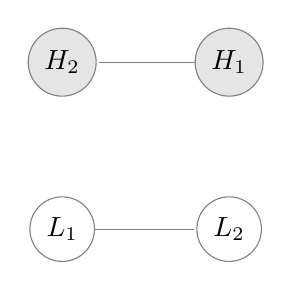
\begin{tikzpicture}[shorten >=1pt,draw=black!50]
	\node (H1) at ( 1.06,  1.06)	[circle, draw, fill = gray!20]	{$H_{1}$};
	\node (H2) at (-1.06,  1.06)	[circle, draw, fill = gray!20]	{$H_{2}$};
	\node (L1) at (-1.06, -1.06)	[circle, draw, fill = white]	{$L_{1}$};
	\node (L2) at ( 1.06, -1.06)	[circle, draw, fill = white]	{$L_{2}$};
	\draw (H1) -- (H2);
	\draw (L1) -- (L2);
\end{tikzpicture}
\end{center}
\columnbreak

\scaleeq{
Equations: \begin{cases}
	e^{H}_{1} \left(\frac{25 \phi}{3} - 3\right) = \alpha + 3 e^{H}_{2} - 2 e^{L}_{1} \theta - 2 e^{L}_{2} \theta - \gamma\\
	e^{H}_{2} \left(\frac{25 \phi}{3} - 3\right) = \alpha + 3 e^{H}_{1} - 2 e^{L}_{1} \theta - 2 e^{L}_{2} \theta - \gamma\\
	e^{L}_{1} \left(\frac{25 \phi}{3 \theta} - 3 \theta\right) = \alpha - 2 e^{H}_{1} - 2 e^{H}_{2} + 3 e^{L}_{2} \theta - \gamma\\
	e^{L}_{2} \left(\frac{25 \phi}{3 \theta} - 3 \theta\right) = \alpha - 2 e^{H}_{1} - 2 e^{H}_{2} + 3 e^{L}_{1} \theta - \gamma
\end{cases}
}\end{multicols}


Optimal efforts:

\scaleeq{
\begin{cases}
	e^{H}_{1} &= \frac{3 \left(\alpha - \gamma\right) \left(5 \phi - 6 \theta^{2}\right)}{125 \phi^{2} - 90 \phi \theta^{2} - 90 \phi + 36 \theta^{2}}\\
	e^{H}_{2} &= \frac{3 \left(\alpha - \gamma\right) \left(5 \phi - 6 \theta^{2}\right)}{125 \phi^{2} - 90 \phi \theta^{2} - 90 \phi + 36 \theta^{2}}\\
	e^{L}_{1} &= \frac{3 \theta \left(\alpha - \gamma\right) \left(5 \phi - 6\right)}{125 \phi^{2} - 90 \phi \theta^{2} - 90 \phi + 36 \theta^{2}}\\
	e^{L}_{2} &= \frac{3 \theta \left(\alpha - \gamma\right) \left(5 \phi - 6\right)}{125 \phi^{2} - 90 \phi \theta^{2} - 90 \phi + 36 \theta^{2}}
\end{cases}
}

Production Costs:

\scaleeq{
\begin{cases}
	c^{H}_{1} &= - \frac{30 \alpha \phi - 36 \alpha \theta^{2} - 125 \gamma \phi^{2} + 90 \gamma \phi \theta^{2} + 60 \gamma \phi}{125 \phi^{2} - 90 \phi \theta^{2} - 90 \phi + 36 \theta^{2}}\\
	c^{H}_{2} &= - \frac{30 \alpha \phi - 36 \alpha \theta^{2} - 125 \gamma \phi^{2} + 90 \gamma \phi \theta^{2} + 60 \gamma \phi}{125 \phi^{2} - 90 \phi \theta^{2} - 90 \phi + 36 \theta^{2}}\\
	c^{L}_{1} &= - \frac{30 \alpha \phi \theta^{2} - 36 \alpha \theta^{2} - 125 \gamma \phi^{2} + 60 \gamma \phi \theta^{2} + 90 \gamma \phi}{125 \phi^{2} - 90 \phi \theta^{2} - 90 \phi + 36 \theta^{2}}\\
	c^{L}_{2} &= - \frac{30 \alpha \phi \theta^{2} - 36 \alpha \theta^{2} - 125 \gamma \phi^{2} + 60 \gamma \phi \theta^{2} + 90 \gamma \phi}{125 \phi^{2} - 90 \phi \theta^{2} - 90 \phi + 36 \theta^{2}}
\end{cases}
}

Production Quantities:

\scaleeq{
\begin{cases}
	q^{H}_{1} &= \frac{5 \phi \left(\alpha - \gamma\right) \left(5 \phi - 6 \theta^{2}\right)}{125 \phi^{2} - 90 \phi \theta^{2} - 90 \phi + 36 \theta^{2}}\\
	q^{H}_{2} &= \frac{5 \phi \left(\alpha - \gamma\right) \left(5 \phi - 6 \theta^{2}\right)}{125 \phi^{2} - 90 \phi \theta^{2} - 90 \phi + 36 \theta^{2}}\\
	q^{L}_{1} &= \frac{5 \phi \left(\alpha - \gamma\right) \left(5 \phi - 6\right)}{125 \phi^{2} - 90 \phi \theta^{2} - 90 \phi + 36 \theta^{2}}\\
	q^{L}_{2} &= \frac{5 \phi \left(\alpha - \gamma\right) \left(5 \phi - 6\right)}{125 \phi^{2} - 90 \phi \theta^{2} - 90 \phi + 36 \theta^{2}}
\end{cases}
}

Profits:

\begin{equation}
\label{eq:E2E:2H2L_profit}
\scaledequation{\begin{cases}
	\pi^{H}_{1} &= \frac{\phi \left(\alpha - \gamma\right)^{2} \left(5 \phi - 6 \theta^{2}\right)^{2} \left(25 \phi - 9\right)}{\left(125 \phi^{2} - 90 \phi \theta^{2} - 90 \phi + 36 \theta^{2}\right)^{2}}\\
	\pi^{H}_{2} &= \frac{\phi \left(\alpha - \gamma\right)^{2} \left(5 \phi - 6 \theta^{2}\right)^{2} \left(25 \phi - 9\right)}{\left(125 \phi^{2} - 90 \phi \theta^{2} - 90 \phi + 36 \theta^{2}\right)^{2}}\\
	\pi^{L}_{1} &= \frac{\phi \left(\alpha - \gamma\right)^{2} \left(5 \phi - 6\right)^{2} \left(25 \phi - 9 \theta^{2}\right)}{\left(125 \phi^{2} - 90 \phi \theta^{2} - 90 \phi + 36 \theta^{2}\right)^{2}}\\
	\pi^{L}_{2} &= \frac{\phi \left(\alpha - \gamma\right)^{2} \left(5 \phi - 6\right)^{2} \left(25 \phi - 9 \theta^{2}\right)}{\left(125 \phi^{2} - 90 \phi \theta^{2} - 90 \phi + 36 \theta^{2}\right)^{2}}
\end{cases}
}
\end{equation}

Total Production:

\scaleeq{
\frac{20 \phi \left(\alpha - \gamma\right) \left(5 \phi - 3 \theta^{2} - 3\right)}{125 \phi^{2} - 90 \phi \theta^{2} - 90 \phi + 36 \theta^{2}}
}

Price:

\scaleeq{
\frac{25 \alpha \phi^{2} - 30 \alpha \phi \theta^{2} - 30 \alpha \phi + 36 \alpha \theta^{2} + 100 \gamma \phi^{2} - 60 \gamma \phi \theta^{2} - 60 \gamma \phi}{125 \phi^{2} - 90 \phi \theta^{2} - 90 \phi + 36 \theta^{2}}
}

Firm Surplus:

\scaleeq{
\frac{2 \phi \left(\alpha - \gamma\right)^{2} \left(1250 \phi^{3} - 1725 \phi^{2} \theta^{2} - 1725 \phi^{2} + 900 \phi \theta^{4} + 1080 \phi \theta^{2} + 900 \phi - 324 \theta^{4} - 324 \theta^{2}\right)}{\left(125 \phi^{2} - 90 \phi \theta^{2} - 90 \phi + 36 \theta^{2}\right)^{2}}
}

Consumer Surplus:

\scaleeq{
\frac{200 \phi^{2} \left(\alpha - \gamma\right)^{2} \left(5 \phi - 3 \theta^{2} - 3\right)^{2}}{\left(125 \phi^{2} - 90 \phi \theta^{2} - 90 \phi + 36 \theta^{2}\right)^{2}}
}

Social Welfare:

\scaleeq{
\frac{6 \phi \left(\alpha - \gamma\right)^{2} \left(1250 \phi^{3} - 1575 \phi^{2} \theta^{2} - 1575 \phi^{2} + 600 \phi \theta^{4} + 960 \phi \theta^{2} + 600 \phi - 108 \theta^{4} - 108 \theta^{2}\right)}{\left(125 \phi^{2} - 90 \phi \theta^{2} - 90 \phi + 36 \theta^{2}\right)^{2}}
}

%======================================================================

\subsubsection{E2F [2H2L]}
\label{apx:E2F:2H2L}

\begin{multicols}{2}
\begin{center}
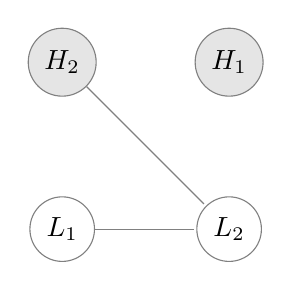
\begin{tikzpicture}[shorten >=1pt,draw=black!50]
	\node (H1) at ( 1.06,  1.06)	[circle, draw, fill = gray!20]	{$H_{1}$};
	\node (H2) at (-1.06,  1.06)	[circle, draw, fill = gray!20]	{$H_{2}$};
	\node (L1) at (-1.06, -1.06)	[circle, draw, fill = white]	{$L_{1}$};
	\node (L2) at ( 1.06, -1.06)	[circle, draw, fill = white]	{$L_{2}$};
	\draw (H2) -- (L2);
	\draw (L1) -- (L2);
\end{tikzpicture}
\end{center}
\columnbreak

\scaleeq{
Equations: \begin{cases}
	e^{H}_{1} \left(\frac{25 \phi}{4} - 4\right) = \alpha - 2 e^{H}_{2} - 2 e^{L}_{1} \theta - 3 e^{L}_{2} \theta - \gamma\\
	e^{H}_{2} \left(\frac{25 \phi}{3} - 3\right) = \alpha - e^{H}_{1} - 2 e^{L}_{1} \theta + 2 e^{L}_{2} \theta - \gamma\\
	e^{L}_{1} \left(\frac{25 \phi}{3 \theta} - 3 \theta\right) = \alpha - e^{H}_{1} - 2 e^{H}_{2} + 2 e^{L}_{2} \theta - \gamma\\
	e^{L}_{2} \left(\frac{25 \phi}{2 \theta} - 2 \theta\right) = \alpha - e^{H}_{1} + 3 e^{H}_{2} + 3 e^{L}_{1} \theta - \gamma
\end{cases}
}\end{multicols}


Optimal efforts:

\scaleeq{
\begin{cases}
	e^{H}_{1} &= \frac{4 \left(\alpha - \gamma\right) \left(125 \phi^{3} - 125 \phi^{2} \theta^{2} - 75 \phi^{2} + 45 \phi \theta^{2} + 18 \theta^{4}\right)}{3125 \phi^{4} - 1625 \phi^{3} \theta^{2} - 3125 \phi^{3} + 1025 \phi^{2} \theta^{2} + 600 \phi^{2} + 180 \phi \theta^{4} - 72 \theta^{4}}\\
	e^{H}_{2} &= \frac{15 \phi \left(\alpha - \gamma\right) \left(5 \phi - 4\right) \left(5 \phi - 3 \theta^{2}\right)}{3125 \phi^{4} - 1625 \phi^{3} \theta^{2} - 3125 \phi^{3} + 1025 \phi^{2} \theta^{2} + 600 \phi^{2} + 180 \phi \theta^{4} - 72 \theta^{4}}\\
	e^{L}_{1} &= \frac{15 \phi \theta \left(\alpha - \gamma\right) \left(5 \phi - 4\right) \left(5 \phi - 3\right)}{3125 \phi^{4} - 1625 \phi^{3} \theta^{2} - 3125 \phi^{3} + 1025 \phi^{2} \theta^{2} + 600 \phi^{2} + 180 \phi \theta^{4} - 72 \theta^{4}}\\
	e^{L}_{2} &= \frac{2 \theta \left(\alpha - \gamma\right) \left(5 \phi - 4\right) \left(5 \phi - 3 \theta\right) \left(5 \phi + 3 \theta\right)}{3125 \phi^{4} - 1625 \phi^{3} \theta^{2} - 3125 \phi^{3} + 1025 \phi^{2} \theta^{2} + 600 \phi^{2} + 180 \phi \theta^{4} - 72 \theta^{4}}
\end{cases}
}

Production Costs:

\scaleeq{
\begin{cases}
	c^{H}_{1} &= - \frac{500 \alpha \phi^{3} - 500 \alpha \phi^{2} \theta^{2} - 300 \alpha \phi^{2} + 180 \alpha \phi \theta^{2} + 72 \alpha \theta^{4} - 3125 \gamma \phi^{4} + 1625 \gamma \phi^{3} \theta^{2} + 2625 \gamma \phi^{3} - 525 \gamma \phi^{2} \theta^{2} - 300 \gamma \phi^{2} - 180 \gamma \phi \theta^{4} - 180 \gamma \phi \theta^{2}}{3125 \phi^{4} - 1625 \phi^{3} \theta^{2} - 3125 \phi^{3} + 1025 \phi^{2} \theta^{2} + 600 \phi^{2} + 180 \phi \theta^{4} - 72 \theta^{4}}\\
	c^{H}_{2} &= - \frac{250 \alpha \phi^{3} \theta^{2} + 375 \alpha \phi^{3} - 425 \alpha \phi^{2} \theta^{2} - 300 \alpha \phi^{2} - 90 \alpha \phi \theta^{4} + 180 \alpha \phi \theta^{2} + 72 \alpha \theta^{4} - 3125 \gamma \phi^{4} + 1375 \gamma \phi^{3} \theta^{2} + 2750 \gamma \phi^{3} - 600 \gamma \phi^{2} \theta^{2} - 300 \gamma \phi^{2} - 90 \gamma \phi \theta^{4} - 180 \gamma \phi \theta^{2}}{3125 \phi^{4} - 1625 \phi^{3} \theta^{2} - 3125 \phi^{3} + 1025 \phi^{2} \theta^{2} + 600 \phi^{2} + 180 \phi \theta^{4} - 72 \theta^{4}}\\
	c^{L}_{1} &= - \frac{625 \alpha \phi^{3} \theta^{2} - 725 \alpha \phi^{2} \theta^{2} - 90 \alpha \phi \theta^{4} + 180 \alpha \phi \theta^{2} + 72 \alpha \theta^{4} - 3125 \gamma \phi^{4} + 1000 \gamma \phi^{3} \theta^{2} + 3125 \gamma \phi^{3} - 300 \gamma \phi^{2} \theta^{2} - 600 \gamma \phi^{2} - 90 \gamma \phi \theta^{4} - 180 \gamma \phi \theta^{2}}{3125 \phi^{4} - 1625 \phi^{3} \theta^{2} - 3125 \phi^{3} + 1025 \phi^{2} \theta^{2} + 600 \phi^{2} + 180 \phi \theta^{4} - 72 \theta^{4}}\\
	c^{L}_{2} &= - \frac{625 \alpha \phi^{3} \theta^{2} + 375 \alpha \phi^{3} - 950 \alpha \phi^{2} \theta^{2} - 300 \alpha \phi^{2} - 90 \alpha \phi \theta^{4} + 360 \alpha \phi \theta^{2} + 72 \alpha \theta^{4} - 3125 \gamma \phi^{4} + 1000 \gamma \phi^{3} \theta^{2} + 2750 \gamma \phi^{3} - 75 \gamma \phi^{2} \theta^{2} - 300 \gamma \phi^{2} - 90 \gamma \phi \theta^{4} - 360 \gamma \phi \theta^{2}}{3125 \phi^{4} - 1625 \phi^{3} \theta^{2} - 3125 \phi^{3} + 1025 \phi^{2} \theta^{2} + 600 \phi^{2} + 180 \phi \theta^{4} - 72 \theta^{4}}
\end{cases}
}

Production Quantities:

\scaleeq{
\begin{cases}
	q^{H}_{1} &= \frac{5 \phi \left(\alpha - \gamma\right) \left(125 \phi^{3} - 125 \phi^{2} \theta^{2} - 75 \phi^{2} + 45 \phi \theta^{2} + 18 \theta^{4}\right)}{3125 \phi^{4} - 1625 \phi^{3} \theta^{2} - 3125 \phi^{3} + 1025 \phi^{2} \theta^{2} + 600 \phi^{2} + 180 \phi \theta^{4} - 72 \theta^{4}}\\
	q^{H}_{2} &= \frac{25 \phi^{2} \left(\alpha - \gamma\right) \left(5 \phi - 4\right) \left(5 \phi - 3 \theta^{2}\right)}{3125 \phi^{4} - 1625 \phi^{3} \theta^{2} - 3125 \phi^{3} + 1025 \phi^{2} \theta^{2} + 600 \phi^{2} + 180 \phi \theta^{4} - 72 \theta^{4}}\\
	q^{L}_{1} &= \frac{25 \phi^{2} \left(\alpha - \gamma\right) \left(5 \phi - 4\right) \left(5 \phi - 3\right)}{3125 \phi^{4} - 1625 \phi^{3} \theta^{2} - 3125 \phi^{3} + 1025 \phi^{2} \theta^{2} + 600 \phi^{2} + 180 \phi \theta^{4} - 72 \theta^{4}}\\
	q^{L}_{2} &= \frac{5 \phi \left(\alpha - \gamma\right) \left(5 \phi - 4\right) \left(5 \phi - 3 \theta\right) \left(5 \phi + 3 \theta\right)}{3125 \phi^{4} - 1625 \phi^{3} \theta^{2} - 3125 \phi^{3} + 1025 \phi^{2} \theta^{2} + 600 \phi^{2} + 180 \phi \theta^{4} - 72 \theta^{4}}
\end{cases}
}

Profits:

\begin{equation}
\label{eq:E2F:2H2L_profit}
\scaledequation{\begin{cases}
	\pi^{H}_{1} &= \frac{\phi \left(\alpha - \gamma\right)^{2} \left(25 \phi - 16\right) \left(125 \phi^{3} - 125 \phi^{2} \theta^{2} - 75 \phi^{2} + 45 \phi \theta^{2} + 18 \theta^{4}\right)^{2}}{\left(3125 \phi^{4} - 1625 \phi^{3} \theta^{2} - 3125 \phi^{3} + 1025 \phi^{2} \theta^{2} + 600 \phi^{2} + 180 \phi \theta^{4} - 72 \theta^{4}\right)^{2}}\\
	\pi^{H}_{2} &= \frac{25 \phi^{3} \left(\alpha - \gamma\right)^{2} \left(5 \phi - 4\right)^{2} \left(5 \phi - 3 \theta^{2}\right)^{2} \left(25 \phi - 9\right)}{\left(3125 \phi^{4} - 1625 \phi^{3} \theta^{2} - 3125 \phi^{3} + 1025 \phi^{2} \theta^{2} + 600 \phi^{2} + 180 \phi \theta^{4} - 72 \theta^{4}\right)^{2}}\\
	\pi^{L}_{1} &= \frac{25 \phi^{3} \left(\alpha - \gamma\right)^{2} \left(5 \phi - 4\right)^{2} \left(5 \phi - 3\right)^{2} \left(25 \phi - 9 \theta^{2}\right)}{\left(3125 \phi^{4} - 1625 \phi^{3} \theta^{2} - 3125 \phi^{3} + 1025 \phi^{2} \theta^{2} + 600 \phi^{2} + 180 \phi \theta^{4} - 72 \theta^{4}\right)^{2}}\\
	\pi^{L}_{2} &= \frac{\phi \left(\alpha - \gamma\right)^{2} \left(5 \phi - 4\right)^{2} \left(5 \phi - 3 \theta\right)^{2} \left(5 \phi + 3 \theta\right)^{2} \left(25 \phi - 4 \theta^{2}\right)}{\left(3125 \phi^{4} - 1625 \phi^{3} \theta^{2} - 3125 \phi^{3} + 1025 \phi^{2} \theta^{2} + 600 \phi^{2} + 180 \phi \theta^{4} - 72 \theta^{4}\right)^{2}}
\end{cases}
}
\end{equation}

Total Production:

\scaleeq{
\frac{10 \phi \left(\alpha - \gamma\right) \left(250 \phi^{3} - 100 \phi^{2} \theta^{2} - 225 \phi^{2} + 30 \phi \theta^{2} + 30 \phi + 9 \theta^{4} + 18 \theta^{2}\right)}{3125 \phi^{4} - 1625 \phi^{3} \theta^{2} - 3125 \phi^{3} + 1025 \phi^{2} \theta^{2} + 600 \phi^{2} + 180 \phi \theta^{4} - 72 \theta^{4}}
}

Price:

\scaleeq{
\frac{625 \alpha \phi^{4} - 625 \alpha \phi^{3} \theta^{2} - 875 \alpha \phi^{3} + 725 \alpha \phi^{2} \theta^{2} + 300 \alpha \phi^{2} + 90 \alpha \phi \theta^{4} - 180 \alpha \phi \theta^{2} - 72 \alpha \theta^{4} + 2500 \gamma \phi^{4} - 1000 \gamma \phi^{3} \theta^{2} - 2250 \gamma \phi^{3} + 300 \gamma \phi^{2} \theta^{2} + 300 \gamma \phi^{2} + 90 \gamma \phi \theta^{4} + 180 \gamma \phi \theta^{2}}{3125 \phi^{4} - 1625 \phi^{3} \theta^{2} - 3125 \phi^{3} + 1025 \phi^{2} \theta^{2} + 600 \phi^{2} + 180 \phi \theta^{4} - 72 \theta^{4}}
}

Firm Surplus:

\scaleeq{
\frac{\phi \left(\alpha - \gamma\right)^{2} \left(1562500 \phi^{7} - 1453125 \phi^{6} \theta^{2} - 3203125 \phi^{6} + 531250 \phi^{5} \theta^{4} + 2381250 \phi^{5} \theta^{2} + 2306250 \phi^{5} - 649375 \phi^{4} \theta^{4} - 1219375 \phi^{4} \theta^{2} - 705000 \phi^{4} - 112500 \phi^{3} \theta^{6} + 240750 \phi^{3} \theta^{4} + 225000 \phi^{3} \theta^{2} + 90000 \phi^{3} + 104400 \phi^{2} \theta^{6} - 73800 \phi^{2} \theta^{4} - 32400 \phi^{2} \theta^{2} + 8100 \phi \theta^{8} - 12960 \phi \theta^{6} + 32400 \phi \theta^{4} - 5184 \theta^{8} - 5184 \theta^{6}\right)}{\left(3125 \phi^{4} - 1625 \phi^{3} \theta^{2} - 3125 \phi^{3} + 1025 \phi^{2} \theta^{2} + 600 \phi^{2} + 180 \phi \theta^{4} - 72 \theta^{4}\right)^{2}}
}

Consumer Surplus:

\scaleeq{
\frac{50 \phi^{2} \left(\alpha - \gamma\right)^{2} \left(250 \phi^{3} - 100 \phi^{2} \theta^{2} - 225 \phi^{2} + 30 \phi \theta^{2} + 30 \phi + 9 \theta^{4} + 18 \theta^{2}\right)^{2}}{\left(3125 \phi^{4} - 1625 \phi^{3} \theta^{2} - 3125 \phi^{3} + 1025 \phi^{2} \theta^{2} + 600 \phi^{2} + 180 \phi \theta^{4} - 72 \theta^{4}\right)^{2}}
}

Social Welfare:

\scaleeq{
\frac{\phi \left(\alpha - \gamma\right)^{2} \left(4687500 \phi^{7} - 3953125 \phi^{6} \theta^{2} - 8828125 \phi^{6} + 1031250 \phi^{5} \theta^{4} + 5381250 \phi^{5} \theta^{2} + 5587500 \phi^{5} - 724375 \phi^{4} \theta^{4} - 1744375 \phi^{4} \theta^{2} - 1380000 \phi^{4} - 202500 \phi^{3} \theta^{6} - 96750 \phi^{3} \theta^{4} - 90000 \phi^{3} \theta^{2} + 135000 \phi^{3} + 131400 \phi^{2} \theta^{6} + 7200 \phi^{2} \theta^{4} + 21600 \phi^{2} \theta^{2} + 12150 \phi \theta^{8} + 3240 \phi \theta^{6} + 48600 \phi \theta^{4} - 5184 \theta^{8} - 5184 \theta^{6}\right)}{\left(3125 \phi^{4} - 1625 \phi^{3} \theta^{2} - 3125 \phi^{3} + 1025 \phi^{2} \theta^{2} + 600 \phi^{2} + 180 \phi \theta^{4} - 72 \theta^{4}\right)^{2}}
}

%======================================================================

\subsubsection{E3A [2H2L]}
\label{apx:E3A:2H2L}

\begin{multicols}{2}
\begin{center}
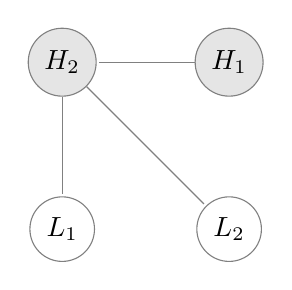
\begin{tikzpicture}[shorten >=1pt,draw=black!50]
	\node (H1) at ( 1.06,  1.06)	[circle, draw, fill = gray!20]	{$H_{1}$};
	\node (H2) at (-1.06,  1.06)	[circle, draw, fill = gray!20]	{$H_{2}$};
	\node (L1) at (-1.06, -1.06)	[circle, draw, fill = white]	{$L_{1}$};
	\node (L2) at ( 1.06, -1.06)	[circle, draw, fill = white]	{$L_{2}$};
	\draw (H1) -- (H2);
	\draw (H2) -- (L1);
	\draw (H2) -- (L2);
\end{tikzpicture}
\end{center}
\columnbreak

\scaleeq{
Equations: \begin{cases}
	e^{H}_{1} \left(\frac{25 \phi}{3} - 3\right) = \alpha + e^{H}_{2} - 2 e^{L}_{1} \theta - 2 e^{L}_{2} \theta - \gamma\\
	e^{H}_{2} \left(25 \phi - 1\right) = \alpha + 3 e^{H}_{1} + 3 e^{L}_{1} \theta + 3 e^{L}_{2} \theta - \gamma\\
	e^{L}_{1} \left(\frac{25 \phi}{3 \theta} - 3 \theta\right) = \alpha - 2 e^{H}_{1} + e^{H}_{2} - 2 e^{L}_{2} \theta - \gamma\\
	e^{L}_{2} \left(\frac{25 \phi}{3 \theta} - 3 \theta\right) = \alpha - 2 e^{H}_{1} + e^{H}_{2} - 2 e^{L}_{1} \theta - \gamma
\end{cases}
}\end{multicols}


Optimal efforts:

\scaleeq{
\begin{cases}
	e^{H}_{1} &= \frac{15 \phi \left(\alpha - \gamma\right) \left(5 \phi - 3 \theta^{2}\right)}{625 \phi^{3} - 75 \phi^{2} \theta^{2} - 250 \phi^{2} - 60 \phi \theta^{2} + 18 \theta^{2}}\\
	e^{H}_{2} &= \frac{\left(\alpha - \gamma\right) \left(25 \phi^{2} + 15 \phi \theta^{2} - 18 \theta^{2}\right)}{625 \phi^{3} - 75 \phi^{2} \theta^{2} - 250 \phi^{2} - 60 \phi \theta^{2} + 18 \theta^{2}}\\
	e^{L}_{1} &= \frac{15 \phi \theta \left(\alpha - \gamma\right) \left(5 \phi - 3\right)}{625 \phi^{3} - 75 \phi^{2} \theta^{2} - 250 \phi^{2} - 60 \phi \theta^{2} + 18 \theta^{2}}\\
	e^{L}_{2} &= \frac{15 \phi \theta \left(\alpha - \gamma\right) \left(5 \phi - 3\right)}{625 \phi^{3} - 75 \phi^{2} \theta^{2} - 250 \phi^{2} - 60 \phi \theta^{2} + 18 \theta^{2}}
\end{cases}
}

Production Costs:

\scaleeq{
\begin{cases}
	c^{H}_{1} &= - \frac{100 \alpha \phi^{2} - 30 \alpha \phi \theta^{2} - 18 \alpha \theta^{2} - 625 \gamma \phi^{3} + 75 \gamma \phi^{2} \theta^{2} + 150 \gamma \phi^{2} + 90 \gamma \phi \theta^{2}}{625 \phi^{3} - 75 \phi^{2} \theta^{2} - 250 \phi^{2} - 60 \phi \theta^{2} + 18 \theta^{2}}\\
	c^{H}_{2} &= - \frac{150 \alpha \phi^{2} \theta^{2} + 100 \alpha \phi^{2} - 120 \alpha \phi \theta^{2} - 18 \alpha \theta^{2} - 625 \gamma \phi^{3} - 75 \gamma \phi^{2} \theta^{2} + 150 \gamma \phi^{2} + 180 \gamma \phi \theta^{2}}{625 \phi^{3} - 75 \phi^{2} \theta^{2} - 250 \phi^{2} - 60 \phi \theta^{2} + 18 \theta^{2}}\\
	c^{L}_{1} &= - \frac{75 \alpha \phi^{2} \theta^{2} + 25 \alpha \phi^{2} - 30 \alpha \phi \theta^{2} - 18 \alpha \theta^{2} - 625 \gamma \phi^{3} + 225 \gamma \phi^{2} + 90 \gamma \phi \theta^{2}}{625 \phi^{3} - 75 \phi^{2} \theta^{2} - 250 \phi^{2} - 60 \phi \theta^{2} + 18 \theta^{2}}\\
	c^{L}_{2} &= - \frac{75 \alpha \phi^{2} \theta^{2} + 25 \alpha \phi^{2} - 30 \alpha \phi \theta^{2} - 18 \alpha \theta^{2} - 625 \gamma \phi^{3} + 225 \gamma \phi^{2} + 90 \gamma \phi \theta^{2}}{625 \phi^{3} - 75 \phi^{2} \theta^{2} - 250 \phi^{2} - 60 \phi \theta^{2} + 18 \theta^{2}}
\end{cases}
}

Production Quantities:

\scaleeq{
\begin{cases}
	q^{H}_{1} &= \frac{25 \phi^{2} \left(\alpha - \gamma\right) \left(5 \phi - 3 \theta^{2}\right)}{625 \phi^{3} - 75 \phi^{2} \theta^{2} - 250 \phi^{2} - 60 \phi \theta^{2} + 18 \theta^{2}}\\
	q^{H}_{2} &= \frac{5 \phi \left(\alpha - \gamma\right) \left(25 \phi^{2} + 15 \phi \theta^{2} - 18 \theta^{2}\right)}{625 \phi^{3} - 75 \phi^{2} \theta^{2} - 250 \phi^{2} - 60 \phi \theta^{2} + 18 \theta^{2}}\\
	q^{L}_{1} &= \frac{25 \phi^{2} \left(\alpha - \gamma\right) \left(5 \phi - 3\right)}{625 \phi^{3} - 75 \phi^{2} \theta^{2} - 250 \phi^{2} - 60 \phi \theta^{2} + 18 \theta^{2}}\\
	q^{L}_{2} &= \frac{25 \phi^{2} \left(\alpha - \gamma\right) \left(5 \phi - 3\right)}{625 \phi^{3} - 75 \phi^{2} \theta^{2} - 250 \phi^{2} - 60 \phi \theta^{2} + 18 \theta^{2}}
\end{cases}
}

Profits:

\begin{equation}
\label{eq:E3A:2H2L_profit}
\scaledequation{\begin{cases}
	\pi^{H}_{1} &= \frac{25 \phi^{3} \left(\alpha - \gamma\right)^{2} \left(5 \phi - 3 \theta^{2}\right)^{2} \left(25 \phi - 9\right)}{\left(625 \phi^{3} - 75 \phi^{2} \theta^{2} - 250 \phi^{2} - 60 \phi \theta^{2} + 18 \theta^{2}\right)^{2}}\\
	\pi^{H}_{2} &= \frac{\phi \left(\alpha - \gamma\right)^{2} \left(25 \phi - 1\right) \left(25 \phi^{2} + 15 \phi \theta^{2} - 18 \theta^{2}\right)^{2}}{\left(625 \phi^{3} - 75 \phi^{2} \theta^{2} - 250 \phi^{2} - 60 \phi \theta^{2} + 18 \theta^{2}\right)^{2}}\\
	\pi^{L}_{1} &= \frac{25 \phi^{3} \left(\alpha - \gamma\right)^{2} \left(5 \phi - 3\right)^{2} \left(25 \phi - 9 \theta^{2}\right)}{\left(625 \phi^{3} - 75 \phi^{2} \theta^{2} - 250 \phi^{2} - 60 \phi \theta^{2} + 18 \theta^{2}\right)^{2}}\\
	\pi^{L}_{2} &= \frac{25 \phi^{3} \left(\alpha - \gamma\right)^{2} \left(5 \phi - 3\right)^{2} \left(25 \phi - 9 \theta^{2}\right)}{\left(625 \phi^{3} - 75 \phi^{2} \theta^{2} - 250 \phi^{2} - 60 \phi \theta^{2} + 18 \theta^{2}\right)^{2}}
\end{cases}
}
\end{equation}

Total Production:

\scaleeq{
\frac{10 \phi \left(\alpha - \gamma\right) \left(50 \phi^{2} - 15 \phi - 9 \theta^{2}\right)}{625 \phi^{3} - 75 \phi^{2} \theta^{2} - 250 \phi^{2} - 60 \phi \theta^{2} + 18 \theta^{2}}
}

Price:

\scaleeq{
\frac{125 \alpha \phi^{3} - 75 \alpha \phi^{2} \theta^{2} - 100 \alpha \phi^{2} + 30 \alpha \phi \theta^{2} + 18 \alpha \theta^{2} + 500 \gamma \phi^{3} - 150 \gamma \phi^{2} - 90 \gamma \phi \theta^{2}}{625 \phi^{3} - 75 \phi^{2} \theta^{2} - 250 \phi^{2} - 60 \phi \theta^{2} + 18 \theta^{2}}
}

Firm Surplus:

\scaleeq{
\frac{2 \phi \left(\alpha - \gamma\right)^{2} \left(31250 \phi^{5} - 5625 \phi^{4} \theta^{2} - 21875 \phi^{4} + 5625 \phi^{3} \theta^{4} - 1500 \phi^{3} \theta^{2} + 5625 \phi^{3} - 7875 \phi^{2} \theta^{4} - 1575 \phi^{2} \theta^{2} + 4320 \phi \theta^{4} - 162 \theta^{4}\right)}{\left(625 \phi^{3} - 75 \phi^{2} \theta^{2} - 250 \phi^{2} - 60 \phi \theta^{2} + 18 \theta^{2}\right)^{2}}
}

Consumer Surplus:

\scaleeq{
\frac{50 \phi^{2} \left(\alpha - \gamma\right)^{2} \left(50 \phi^{2} - 15 \phi - 9 \theta^{2}\right)^{2}}{\left(625 \phi^{3} - 75 \phi^{2} \theta^{2} - 250 \phi^{2} - 60 \phi \theta^{2} + 18 \theta^{2}\right)^{2}}
}

Social Welfare:

\scaleeq{
\frac{2 \phi \left(\alpha - \gamma\right)^{2} \left(93750 \phi^{5} - 5625 \phi^{4} \theta^{2} - 59375 \phi^{4} + 5625 \phi^{3} \theta^{4} - 24000 \phi^{3} \theta^{2} + 11250 \phi^{3} - 7875 \phi^{2} \theta^{4} + 5175 \phi^{2} \theta^{2} + 6345 \phi \theta^{4} - 162 \theta^{4}\right)}{\left(625 \phi^{3} - 75 \phi^{2} \theta^{2} - 250 \phi^{2} - 60 \phi \theta^{2} + 18 \theta^{2}\right)^{2}}
}

%======================================================================

\subsubsection{E3B [2H2L]}
\label{apx:E3B:2H2L}

\begin{multicols}{2}
\begin{center}
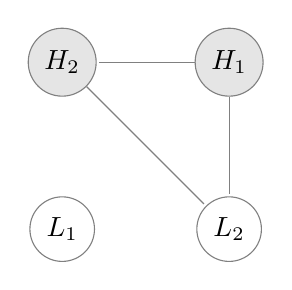
\begin{tikzpicture}[shorten >=1pt,draw=black!50]
	\node (H1) at ( 1.06,  1.06)	[circle, draw, fill = gray!20]	{$H_{1}$};
	\node (H2) at (-1.06,  1.06)	[circle, draw, fill = gray!20]	{$H_{2}$};
	\node (L1) at (-1.06, -1.06)	[circle, draw, fill = white]	{$L_{1}$};
	\node (L2) at ( 1.06, -1.06)	[circle, draw, fill = white]	{$L_{2}$};
	\draw (H1) -- (H2);
	\draw (H1) -- (L2);
	\draw (H2) -- (L2);
\end{tikzpicture}
\end{center}
\columnbreak

\scaleeq{
Equations: \begin{cases}
	e^{H}_{1} \left(\frac{25 \phi}{2} - 2\right) = \alpha + 2 e^{H}_{2} - e^{L}_{1} \theta + 2 e^{L}_{2} \theta - \gamma\\
	e^{H}_{2} \left(\frac{25 \phi}{2} - 2\right) = \alpha + 2 e^{H}_{1} - e^{L}_{1} \theta + 2 e^{L}_{2} \theta - \gamma\\
	e^{L}_{1} \left(\frac{25 \phi}{4 \theta} - 4 \theta\right) = \alpha - 3 e^{H}_{1} - 3 e^{H}_{2} - 3 e^{L}_{2} \theta - \gamma\\
	e^{L}_{2} \left(\frac{25 \phi}{2 \theta} - 2 \theta\right) = \alpha + 2 e^{H}_{1} + 2 e^{H}_{2} - e^{L}_{1} \theta - \gamma
\end{cases}
}\end{multicols}


Optimal efforts:

\scaleeq{
\begin{cases}
	e^{H}_{1} &= \frac{2 \left(\alpha - \gamma\right) \left(5 \phi - 4 \theta^{2}\right)}{125 \phi^{2} - 100 \phi \theta^{2} - 40 \phi + 8 \theta^{4} + 16 \theta^{2}}\\
	e^{H}_{2} &= \frac{2 \left(\alpha - \gamma\right) \left(5 \phi - 4 \theta^{2}\right)}{125 \phi^{2} - 100 \phi \theta^{2} - 40 \phi + 8 \theta^{4} + 16 \theta^{2}}\\
	e^{L}_{1} &= \frac{4 \theta \left(\alpha - \gamma\right) \left(5 \phi - 2 \theta^{2} - 4\right)}{125 \phi^{2} - 100 \phi \theta^{2} - 40 \phi + 8 \theta^{4} + 16 \theta^{2}}\\
	e^{L}_{2} &= \frac{2 \theta \left(\alpha - \gamma\right) \left(5 \phi - 4 \theta^{2}\right)}{125 \phi^{2} - 100 \phi \theta^{2} - 40 \phi + 8 \theta^{4} + 16 \theta^{2}}
\end{cases}
}

Production Costs:

\scaleeq{
\begin{cases}
	c^{H}_{1} &= - \frac{10 \alpha \phi \theta^{2} + 20 \alpha \phi - 8 \alpha \theta^{4} - 16 \alpha \theta^{2} - 125 \gamma \phi^{2} + 90 \gamma \phi \theta^{2} + 20 \gamma \phi}{125 \phi^{2} - 100 \phi \theta^{2} - 40 \phi + 8 \theta^{4} + 16 \theta^{2}}\\
	c^{H}_{2} &= - \frac{10 \alpha \phi \theta^{2} + 20 \alpha \phi - 8 \alpha \theta^{4} - 16 \alpha \theta^{2} - 125 \gamma \phi^{2} + 90 \gamma \phi \theta^{2} + 20 \gamma \phi}{125 \phi^{2} - 100 \phi \theta^{2} - 40 \phi + 8 \theta^{4} + 16 \theta^{2}}\\
	c^{L}_{1} &= - \frac{20 \alpha \phi \theta^{2} - 8 \alpha \theta^{4} - 16 \alpha \theta^{2} - 125 \gamma \phi^{2} + 80 \gamma \phi \theta^{2} + 40 \gamma \phi}{125 \phi^{2} - 100 \phi \theta^{2} - 40 \phi + 8 \theta^{4} + 16 \theta^{2}}\\
	c^{L}_{2} &= - \frac{10 \alpha \phi \theta^{2} + 20 \alpha \phi - 8 \alpha \theta^{4} - 16 \alpha \theta^{2} - 125 \gamma \phi^{2} + 90 \gamma \phi \theta^{2} + 20 \gamma \phi}{125 \phi^{2} - 100 \phi \theta^{2} - 40 \phi + 8 \theta^{4} + 16 \theta^{2}}
\end{cases}
}

Production Quantities:

\scaleeq{
\begin{cases}
	q^{H}_{1} &= \frac{5 \phi \left(\alpha - \gamma\right) \left(5 \phi - 4 \theta^{2}\right)}{125 \phi^{2} - 100 \phi \theta^{2} - 40 \phi + 8 \theta^{4} + 16 \theta^{2}}\\
	q^{H}_{2} &= \frac{5 \phi \left(\alpha - \gamma\right) \left(5 \phi - 4 \theta^{2}\right)}{125 \phi^{2} - 100 \phi \theta^{2} - 40 \phi + 8 \theta^{4} + 16 \theta^{2}}\\
	q^{L}_{1} &= \frac{5 \phi \left(\alpha - \gamma\right) \left(5 \phi - 2 \theta^{2} - 4\right)}{125 \phi^{2} - 100 \phi \theta^{2} - 40 \phi + 8 \theta^{4} + 16 \theta^{2}}\\
	q^{L}_{2} &= \frac{5 \phi \left(\alpha - \gamma\right) \left(5 \phi - 4 \theta^{2}\right)}{125 \phi^{2} - 100 \phi \theta^{2} - 40 \phi + 8 \theta^{4} + 16 \theta^{2}}
\end{cases}
}

Profits:

\begin{equation}
\label{eq:E3B:2H2L_profit}
\scaledequation{\begin{cases}
	\pi^{H}_{1} &= \frac{\phi \left(\alpha - \gamma\right)^{2} \left(5 \phi - 4 \theta^{2}\right)^{2} \left(25 \phi - 4\right)}{\left(125 \phi^{2} - 100 \phi \theta^{2} - 40 \phi + 8 \theta^{4} + 16 \theta^{2}\right)^{2}}\\
	\pi^{H}_{2} &= \frac{\phi \left(\alpha - \gamma\right)^{2} \left(5 \phi - 4 \theta^{2}\right)^{2} \left(25 \phi - 4\right)}{\left(125 \phi^{2} - 100 \phi \theta^{2} - 40 \phi + 8 \theta^{4} + 16 \theta^{2}\right)^{2}}\\
	\pi^{L}_{1} &= \frac{\phi \left(\alpha - \gamma\right)^{2} \left(25 \phi - 16 \theta^{2}\right) \left(5 \phi - 2 \theta^{2} - 4\right)^{2}}{\left(125 \phi^{2} - 100 \phi \theta^{2} - 40 \phi + 8 \theta^{4} + 16 \theta^{2}\right)^{2}}\\
	\pi^{L}_{2} &= \frac{\phi \left(\alpha - \gamma\right)^{2} \left(5 \phi - 4 \theta^{2}\right)^{2} \left(25 \phi - 4 \theta^{2}\right)}{\left(125 \phi^{2} - 100 \phi \theta^{2} - 40 \phi + 8 \theta^{4} + 16 \theta^{2}\right)^{2}}
\end{cases}
}
\end{equation}

Total Production:

\scaleeq{
\frac{10 \phi \left(\alpha - \gamma\right) \left(10 \phi - 7 \theta^{2} - 2\right)}{125 \phi^{2} - 100 \phi \theta^{2} - 40 \phi + 8 \theta^{4} + 16 \theta^{2}}
}

Price:

\scaleeq{
\frac{25 \alpha \phi^{2} - 30 \alpha \phi \theta^{2} - 20 \alpha \phi + 8 \alpha \theta^{4} + 16 \alpha \theta^{2} + 100 \gamma \phi^{2} - 70 \gamma \phi \theta^{2} - 20 \gamma \phi}{125 \phi^{2} - 100 \phi \theta^{2} - 40 \phi + 8 \theta^{4} + 16 \theta^{2}}
}

Firm Surplus:

\scaleeq{
\frac{4 \phi \left(\alpha - \gamma\right)^{2} \left(625 \phi^{3} - 1000 \phi^{2} \theta^{2} - 300 \phi^{2} + 445 \phi \theta^{4} + 340 \phi \theta^{2} + 100 \phi - 32 \theta^{6} - 96 \theta^{4} - 64 \theta^{2}\right)}{\left(125 \phi^{2} - 100 \phi \theta^{2} - 40 \phi + 8 \theta^{4} + 16 \theta^{2}\right)^{2}}
}

Consumer Surplus:

\scaleeq{
\frac{50 \phi^{2} \left(\alpha - \gamma\right)^{2} \left(10 \phi - 7 \theta^{2} - 2\right)^{2}}{\left(125 \phi^{2} - 100 \phi \theta^{2} - 40 \phi + 8 \theta^{4} + 16 \theta^{2}\right)^{2}}
}

Social Welfare:

\scaleeq{
\frac{2 \phi \left(\alpha - \gamma\right)^{2} \left(3750 \phi^{3} - 5500 \phi^{2} \theta^{2} - 1600 \phi^{2} + 2115 \phi \theta^{4} + 1380 \phi \theta^{2} + 300 \phi - 64 \theta^{6} - 192 \theta^{4} - 128 \theta^{2}\right)}{\left(125 \phi^{2} - 100 \phi \theta^{2} - 40 \phi + 8 \theta^{4} + 16 \theta^{2}\right)^{2}}
}

%======================================================================

\subsubsection{E3C [2H2L]}
\label{apx:E3C:2H2L}

\begin{multicols}{2}
\begin{center}
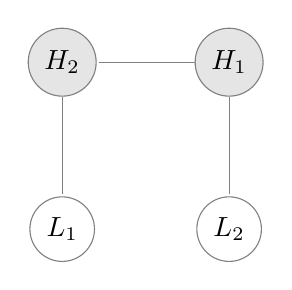
\begin{tikzpicture}[shorten >=1pt,draw=black!50]
	\node (H1) at ( 1.06,  1.06)	[circle, draw, fill = gray!20]	{$H_{1}$};
	\node (H2) at (-1.06,  1.06)	[circle, draw, fill = gray!20]	{$H_{2}$};
	\node (L1) at (-1.06, -1.06)	[circle, draw, fill = white]	{$L_{1}$};
	\node (L2) at ( 1.06, -1.06)	[circle, draw, fill = white]	{$L_{2}$};
	\draw (H1) -- (H2);
	\draw (H1) -- (L2);
	\draw (H2) -- (L1);
\end{tikzpicture}
\end{center}
\columnbreak

\scaleeq{
Equations: \begin{cases}
	e^{H}_{1} \left(\frac{25 \phi}{2} - 2\right) = \alpha + 2 e^{H}_{2} - 2 e^{L}_{1} \theta + 3 e^{L}_{2} \theta - \gamma\\
	e^{H}_{2} \left(\frac{25 \phi}{2} - 2\right) = \alpha + 2 e^{H}_{1} + 3 e^{L}_{1} \theta - 2 e^{L}_{2} \theta - \gamma\\
	e^{L}_{1} \left(\frac{25 \phi}{3 \theta} - 3 \theta\right) = \alpha - 3 e^{H}_{1} + 2 e^{H}_{2} - 2 e^{L}_{2} \theta - \gamma\\
	e^{L}_{2} \left(\frac{25 \phi}{3 \theta} - 3 \theta\right) = \alpha + 2 e^{H}_{1} - 3 e^{H}_{2} - 2 e^{L}_{1} \theta - \gamma
\end{cases}
}\end{multicols}


Optimal efforts:

\scaleeq{
\begin{cases}
	e^{H}_{1} &= \frac{10 \phi \left(\alpha - \gamma\right)}{125 \phi^{2} - 15 \phi \theta^{2} - 40 \phi + 6 \theta^{2}}\\
	e^{H}_{2} &= \frac{10 \phi \left(\alpha - \gamma\right)}{125 \phi^{2} - 15 \phi \theta^{2} - 40 \phi + 6 \theta^{2}}\\
	e^{L}_{1} &= \frac{3 \theta \left(\alpha - \gamma\right) \left(5 \phi - 2\right)}{125 \phi^{2} - 15 \phi \theta^{2} - 40 \phi + 6 \theta^{2}}\\
	e^{L}_{2} &= \frac{3 \theta \left(\alpha - \gamma\right) \left(5 \phi - 2\right)}{125 \phi^{2} - 15 \phi \theta^{2} - 40 \phi + 6 \theta^{2}}
\end{cases}
}

Production Costs:

\scaleeq{
\begin{cases}
	c^{H}_{1} &= - \frac{15 \alpha \phi \theta^{2} + 20 \alpha \phi - 6 \alpha \theta^{2} - 125 \gamma \phi^{2} + 20 \gamma \phi}{125 \phi^{2} - 15 \phi \theta^{2} - 40 \phi + 6 \theta^{2}}\\
	c^{H}_{2} &= - \frac{15 \alpha \phi \theta^{2} + 20 \alpha \phi - 6 \alpha \theta^{2} - 125 \gamma \phi^{2} + 20 \gamma \phi}{125 \phi^{2} - 15 \phi \theta^{2} - 40 \phi + 6 \theta^{2}}\\
	c^{L}_{1} &= - \frac{15 \alpha \phi \theta^{2} + 10 \alpha \phi - 6 \alpha \theta^{2} - 125 \gamma \phi^{2} + 30 \gamma \phi}{125 \phi^{2} - 15 \phi \theta^{2} - 40 \phi + 6 \theta^{2}}\\
	c^{L}_{2} &= - \frac{15 \alpha \phi \theta^{2} + 10 \alpha \phi - 6 \alpha \theta^{2} - 125 \gamma \phi^{2} + 30 \gamma \phi}{125 \phi^{2} - 15 \phi \theta^{2} - 40 \phi + 6 \theta^{2}}
\end{cases}
}

Production Quantities:

\scaleeq{
\begin{cases}
	q^{H}_{1} &= \frac{25 \phi^{2} \left(\alpha - \gamma\right)}{125 \phi^{2} - 15 \phi \theta^{2} - 40 \phi + 6 \theta^{2}}\\
	q^{H}_{2} &= \frac{25 \phi^{2} \left(\alpha - \gamma\right)}{125 \phi^{2} - 15 \phi \theta^{2} - 40 \phi + 6 \theta^{2}}\\
	q^{L}_{1} &= \frac{5 \phi \left(\alpha - \gamma\right) \left(5 \phi - 2\right)}{125 \phi^{2} - 15 \phi \theta^{2} - 40 \phi + 6 \theta^{2}}\\
	q^{L}_{2} &= \frac{5 \phi \left(\alpha - \gamma\right) \left(5 \phi - 2\right)}{125 \phi^{2} - 15 \phi \theta^{2} - 40 \phi + 6 \theta^{2}}
\end{cases}
}

Profits:

\begin{equation}
\label{eq:E3C:2H2L_profit}
\scaledequation{\begin{cases}
	\pi^{H}_{1} &= \frac{25 \phi^{3} \left(\alpha - \gamma\right)^{2} \left(25 \phi - 4\right)}{\left(125 \phi^{2} - 15 \phi \theta^{2} - 40 \phi + 6 \theta^{2}\right)^{2}}\\
	\pi^{H}_{2} &= \frac{25 \phi^{3} \left(\alpha - \gamma\right)^{2} \left(25 \phi - 4\right)}{\left(125 \phi^{2} - 15 \phi \theta^{2} - 40 \phi + 6 \theta^{2}\right)^{2}}\\
	\pi^{L}_{1} &= \frac{\phi \left(\alpha - \gamma\right)^{2} \left(5 \phi - 2\right)^{2} \left(25 \phi - 9 \theta^{2}\right)}{\left(125 \phi^{2} - 15 \phi \theta^{2} - 40 \phi + 6 \theta^{2}\right)^{2}}\\
	\pi^{L}_{2} &= \frac{\phi \left(\alpha - \gamma\right)^{2} \left(5 \phi - 2\right)^{2} \left(25 \phi - 9 \theta^{2}\right)}{\left(125 \phi^{2} - 15 \phi \theta^{2} - 40 \phi + 6 \theta^{2}\right)^{2}}
\end{cases}
}
\end{equation}

Total Production:

\scaleeq{
\frac{20 \phi \left(\alpha - \gamma\right) \left(5 \phi - 1\right)}{125 \phi^{2} - 15 \phi \theta^{2} - 40 \phi + 6 \theta^{2}}
}

Price:

\scaleeq{
\frac{25 \alpha \phi^{2} - 15 \alpha \phi \theta^{2} - 20 \alpha \phi + 6 \alpha \theta^{2} + 100 \gamma \phi^{2} - 20 \gamma \phi}{125 \phi^{2} - 15 \phi \theta^{2} - 40 \phi + 6 \theta^{2}}
}

Firm Surplus:

\scaleeq{
\frac{2 \phi \left(\alpha - \gamma\right)^{2} \left(1250 \phi^{3} - 225 \phi^{2} \theta^{2} - 600 \phi^{2} + 180 \phi \theta^{2} + 100 \phi - 36 \theta^{2}\right)}{\left(125 \phi^{2} - 15 \phi \theta^{2} - 40 \phi + 6 \theta^{2}\right)^{2}}
}

Consumer Surplus:

\scaleeq{
\frac{200 \phi^{2} \left(\alpha - \gamma\right)^{2} \left(5 \phi - 1\right)^{2}}{\left(125 \phi^{2} - 15 \phi \theta^{2} - 40 \phi + 6 \theta^{2}\right)^{2}}
}

Social Welfare:

\scaleeq{
\frac{2 \phi \left(\alpha - \gamma\right)^{2} \left(3750 \phi^{3} - 225 \phi^{2} \theta^{2} - 1600 \phi^{2} + 180 \phi \theta^{2} + 200 \phi - 36 \theta^{2}\right)}{\left(125 \phi^{2} - 15 \phi \theta^{2} - 40 \phi + 6 \theta^{2}\right)^{2}}
}

%======================================================================

\subsubsection{E3D [2H2L]}
\label{apx:E3D:2H2L}

\begin{multicols}{2}
\begin{center}
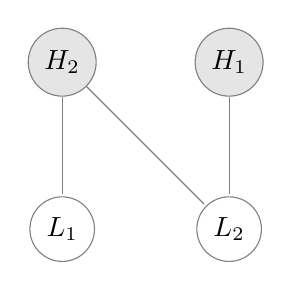
\begin{tikzpicture}[shorten >=1pt,draw=black!50]
	\node (H1) at ( 1.06,  1.06)	[circle, draw, fill = gray!20]	{$H_{1}$};
	\node (H2) at (-1.06,  1.06)	[circle, draw, fill = gray!20]	{$H_{2}$};
	\node (L1) at (-1.06, -1.06)	[circle, draw, fill = white]	{$L_{1}$};
	\node (L2) at ( 1.06, -1.06)	[circle, draw, fill = white]	{$L_{2}$};
	\draw (H1) -- (L2);
	\draw (H2) -- (L1);
	\draw (H2) -- (L2);
\end{tikzpicture}
\end{center}
\columnbreak

\scaleeq{
Equations: \begin{cases}
	e^{H}_{1} \left(\frac{25 \phi}{3} - 3\right) = \alpha - 3 e^{H}_{2} - 2 e^{L}_{1} \theta + 2 e^{L}_{2} \theta - \gamma\\
	e^{H}_{2} \left(\frac{25 \phi}{2} - 2\right) = \alpha - 2 e^{H}_{1} + 3 e^{L}_{1} \theta + 2 e^{L}_{2} \theta - \gamma\\
	e^{L}_{1} \left(\frac{25 \phi}{3 \theta} - 3 \theta\right) = \alpha - 2 e^{H}_{1} + 2 e^{H}_{2} - 3 e^{L}_{2} \theta - \gamma\\
	e^{L}_{2} \left(\frac{25 \phi}{2 \theta} - 2 \theta\right) = \alpha + 3 e^{H}_{1} + 2 e^{H}_{2} - 2 e^{L}_{1} \theta - \gamma
\end{cases}
}\end{multicols}


Optimal efforts:

\scaleeq{
\begin{cases}
	e^{H}_{1} &= \frac{3 \left(\alpha - \gamma\right) \left(125 \phi^{3} - 75 \phi^{2} \theta^{2} - 50 \phi^{2} + 12 \theta^{4}\right)}{3125 \phi^{4} - 1625 \phi^{3} \theta^{2} - 1625 \phi^{3} + 225 \phi^{2} \theta^{2} + 120 \phi \theta^{4} + 120 \phi \theta^{2} - 36 \theta^{4}}\\
	e^{H}_{2} &= \frac{10 \phi \left(\alpha - \gamma\right) \left(25 \phi^{2} - 15 \phi - 6 \theta^{4}\right)}{3125 \phi^{4} - 1625 \phi^{3} \theta^{2} - 1625 \phi^{3} + 225 \phi^{2} \theta^{2} + 120 \phi \theta^{4} + 120 \phi \theta^{2} - 36 \theta^{4}}\\
	e^{L}_{1} &= \frac{3 \theta \left(\alpha - \gamma\right) \left(125 \phi^{3} - 50 \phi^{2} \theta^{2} - 75 \phi^{2} + 12 \theta^{2}\right)}{3125 \phi^{4} - 1625 \phi^{3} \theta^{2} - 1625 \phi^{3} + 225 \phi^{2} \theta^{2} + 120 \phi \theta^{4} + 120 \phi \theta^{2} - 36 \theta^{4}}\\
	e^{L}_{2} &= \frac{10 \phi \theta \left(\alpha - \gamma\right) \left(25 \phi^{2} - 15 \phi \theta^{2} - 6\right)}{3125 \phi^{4} - 1625 \phi^{3} \theta^{2} - 1625 \phi^{3} + 225 \phi^{2} \theta^{2} + 120 \phi \theta^{4} + 120 \phi \theta^{2} - 36 \theta^{4}}
\end{cases}
}

Production Costs:

\scaleeq{
\begin{cases}
	c^{H}_{1} &= - \frac{250 \alpha \phi^{3} \theta^{2} + 375 \alpha \phi^{3} - 150 \alpha \phi^{2} \theta^{4} - 225 \alpha \phi^{2} \theta^{2} - 150 \alpha \phi^{2} - 60 \alpha \phi \theta^{2} + 36 \alpha \theta^{4} - 3125 \gamma \phi^{4} + 1375 \gamma \phi^{3} \theta^{2} + 1250 \gamma \phi^{3} + 150 \gamma \phi^{2} \theta^{4} + 150 \gamma \phi^{2} - 120 \gamma \phi \theta^{4} - 60 \gamma \phi \theta^{2}}{3125 \phi^{4} - 1625 \phi^{3} \theta^{2} - 1625 \phi^{3} + 225 \phi^{2} \theta^{2} + 120 \phi \theta^{4} + 120 \phi \theta^{2} - 36 \theta^{4}}\\
	c^{H}_{2} &= - \frac{625 \alpha \phi^{3} \theta^{2} + 250 \alpha \phi^{3} - 300 \alpha \phi^{2} \theta^{4} - 225 \alpha \phi^{2} \theta^{2} - 150 \alpha \phi^{2} - 60 \alpha \phi \theta^{4} - 60 \alpha \phi \theta^{2} + 36 \alpha \theta^{4} - 3125 \gamma \phi^{4} + 1000 \gamma \phi^{3} \theta^{2} + 1375 \gamma \phi^{3} + 300 \gamma \phi^{2} \theta^{4} + 150 \gamma \phi^{2} - 60 \gamma \phi \theta^{4} - 60 \gamma \phi \theta^{2}}{3125 \phi^{4} - 1625 \phi^{3} \theta^{2} - 1625 \phi^{3} + 225 \phi^{2} \theta^{2} + 120 \phi \theta^{4} + 120 \phi \theta^{2} - 36 \theta^{4}}\\
	c^{L}_{1} &= - \frac{375 \alpha \phi^{3} \theta^{2} + 250 \alpha \phi^{3} - 150 \alpha \phi^{2} \theta^{4} - 225 \alpha \phi^{2} \theta^{2} - 150 \alpha \phi^{2} - 60 \alpha \phi \theta^{4} + 36 \alpha \theta^{4} - 3125 \gamma \phi^{4} + 1250 \gamma \phi^{3} \theta^{2} + 1375 \gamma \phi^{3} + 150 \gamma \phi^{2} \theta^{4} + 150 \gamma \phi^{2} - 60 \gamma \phi \theta^{4} - 120 \gamma \phi \theta^{2}}{3125 \phi^{4} - 1625 \phi^{3} \theta^{2} - 1625 \phi^{3} + 225 \phi^{2} \theta^{2} + 120 \phi \theta^{4} + 120 \phi \theta^{2} - 36 \theta^{4}}\\
	c^{L}_{2} &= - \frac{250 \alpha \phi^{3} \theta^{2} + 625 \alpha \phi^{3} - 150 \alpha \phi^{2} \theta^{4} - 225 \alpha \phi^{2} \theta^{2} - 300 \alpha \phi^{2} - 60 \alpha \phi \theta^{4} - 60 \alpha \phi \theta^{2} + 36 \alpha \theta^{4} - 3125 \gamma \phi^{4} + 1375 \gamma \phi^{3} \theta^{2} + 1000 \gamma \phi^{3} + 150 \gamma \phi^{2} \theta^{4} + 300 \gamma \phi^{2} - 60 \gamma \phi \theta^{4} - 60 \gamma \phi \theta^{2}}{3125 \phi^{4} - 1625 \phi^{3} \theta^{2} - 1625 \phi^{3} + 225 \phi^{2} \theta^{2} + 120 \phi \theta^{4} + 120 \phi \theta^{2} - 36 \theta^{4}}
\end{cases}
}

Production Quantities:

\scaleeq{
\begin{cases}
	q^{H}_{1} &= \frac{5 \phi \left(\alpha - \gamma\right) \left(125 \phi^{3} - 75 \phi^{2} \theta^{2} - 50 \phi^{2} + 12 \theta^{4}\right)}{3125 \phi^{4} - 1625 \phi^{3} \theta^{2} - 1625 \phi^{3} + 225 \phi^{2} \theta^{2} + 120 \phi \theta^{4} + 120 \phi \theta^{2} - 36 \theta^{4}}\\
	q^{H}_{2} &= \frac{25 \phi^{2} \left(\alpha - \gamma\right) \left(25 \phi^{2} - 15 \phi - 6 \theta^{4}\right)}{3125 \phi^{4} - 1625 \phi^{3} \theta^{2} - 1625 \phi^{3} + 225 \phi^{2} \theta^{2} + 120 \phi \theta^{4} + 120 \phi \theta^{2} - 36 \theta^{4}}\\
	q^{L}_{1} &= \frac{5 \phi \left(\alpha - \gamma\right) \left(125 \phi^{3} - 50 \phi^{2} \theta^{2} - 75 \phi^{2} + 12 \theta^{2}\right)}{3125 \phi^{4} - 1625 \phi^{3} \theta^{2} - 1625 \phi^{3} + 225 \phi^{2} \theta^{2} + 120 \phi \theta^{4} + 120 \phi \theta^{2} - 36 \theta^{4}}\\
	q^{L}_{2} &= \frac{25 \phi^{2} \left(\alpha - \gamma\right) \left(25 \phi^{2} - 15 \phi \theta^{2} - 6\right)}{3125 \phi^{4} - 1625 \phi^{3} \theta^{2} - 1625 \phi^{3} + 225 \phi^{2} \theta^{2} + 120 \phi \theta^{4} + 120 \phi \theta^{2} - 36 \theta^{4}}
\end{cases}
}

Profits:

\begin{equation}
\label{eq:E3D:2H2L_profit}
\scaledequation{\begin{cases}
	\pi^{H}_{1} &= \frac{\phi \left(\alpha - \gamma\right)^{2} \left(25 \phi - 9\right) \left(125 \phi^{3} - 75 \phi^{2} \theta^{2} - 50 \phi^{2} + 12 \theta^{4}\right)^{2}}{\left(3125 \phi^{4} - 1625 \phi^{3} \theta^{2} - 1625 \phi^{3} + 225 \phi^{2} \theta^{2} + 120 \phi \theta^{4} + 120 \phi \theta^{2} - 36 \theta^{4}\right)^{2}}\\
	\pi^{H}_{2} &= \frac{25 \phi^{3} \left(\alpha - \gamma\right)^{2} \left(25 \phi - 4\right) \left(25 \phi^{2} - 15 \phi - 6 \theta^{4}\right)^{2}}{\left(3125 \phi^{4} - 1625 \phi^{3} \theta^{2} - 1625 \phi^{3} + 225 \phi^{2} \theta^{2} + 120 \phi \theta^{4} + 120 \phi \theta^{2} - 36 \theta^{4}\right)^{2}}\\
	\pi^{L}_{1} &= \frac{\phi \left(\alpha - \gamma\right)^{2} \left(25 \phi - 9 \theta^{2}\right) \left(125 \phi^{3} - 50 \phi^{2} \theta^{2} - 75 \phi^{2} + 12 \theta^{2}\right)^{2}}{\left(3125 \phi^{4} - 1625 \phi^{3} \theta^{2} - 1625 \phi^{3} + 225 \phi^{2} \theta^{2} + 120 \phi \theta^{4} + 120 \phi \theta^{2} - 36 \theta^{4}\right)^{2}}\\
	\pi^{L}_{2} &= \frac{25 \phi^{3} \left(\alpha - \gamma\right)^{2} \left(25 \phi - 4 \theta^{2}\right) \left(25 \phi^{2} - 15 \phi \theta^{2} - 6\right)^{2}}{\left(3125 \phi^{4} - 1625 \phi^{3} \theta^{2} - 1625 \phi^{3} + 225 \phi^{2} \theta^{2} + 120 \phi \theta^{4} + 120 \phi \theta^{2} - 36 \theta^{4}\right)^{2}}
\end{cases}
}
\end{equation}

Total Production:

\scaleeq{
\frac{10 \phi \left(\alpha - \gamma\right) \left(250 \phi^{3} - 100 \phi^{2} \theta^{2} - 100 \phi^{2} - 15 \phi \theta^{4} - 15 \phi + 6 \theta^{4} + 6 \theta^{2}\right)}{3125 \phi^{4} - 1625 \phi^{3} \theta^{2} - 1625 \phi^{3} + 225 \phi^{2} \theta^{2} + 120 \phi \theta^{4} + 120 \phi \theta^{2} - 36 \theta^{4}}
}

Price:

\scaleeq{
\frac{625 \alpha \phi^{4} - 625 \alpha \phi^{3} \theta^{2} - 625 \alpha \phi^{3} + 150 \alpha \phi^{2} \theta^{4} + 225 \alpha \phi^{2} \theta^{2} + 150 \alpha \phi^{2} + 60 \alpha \phi \theta^{4} + 60 \alpha \phi \theta^{2} - 36 \alpha \theta^{4} + 2500 \gamma \phi^{4} - 1000 \gamma \phi^{3} \theta^{2} - 1000 \gamma \phi^{3} - 150 \gamma \phi^{2} \theta^{4} - 150 \gamma \phi^{2} + 60 \gamma \phi \theta^{4} + 60 \gamma \phi \theta^{2}}{3125 \phi^{4} - 1625 \phi^{3} \theta^{2} - 1625 \phi^{3} + 225 \phi^{2} \theta^{2} + 120 \phi \theta^{4} + 120 \phi \theta^{2} - 36 \theta^{4}}
}

Firm Surplus:

\scaleeq{
\frac{\phi \left(\alpha - \gamma\right)^{2} \left(1562500 \phi^{7} - 1453125 \phi^{6} \theta^{2} - 1453125 \phi^{6} + 343750 \phi^{5} \theta^{4} + 712500 \phi^{5} \theta^{2} + 343750 \phi^{5} - 45000 \phi^{4} \theta^{6} + 99375 \phi^{4} \theta^{4} + 99375 \phi^{4} \theta^{2} - 45000 \phi^{4} + 22500 \phi^{3} \theta^{8} - 45000 \phi^{3} \theta^{6} - 150000 \phi^{3} \theta^{4} - 45000 \phi^{3} \theta^{2} + 22500 \phi^{3} - 3600 \phi^{2} \theta^{8} + 27000 \phi^{2} \theta^{6} + 27000 \phi^{2} \theta^{4} - 3600 \phi^{2} \theta^{2} + 3600 \phi \theta^{8} + 3600 \phi \theta^{4} - 1296 \theta^{8} - 1296 \theta^{6}\right)}{\left(3125 \phi^{4} - 1625 \phi^{3} \theta^{2} - 1625 \phi^{3} + 225 \phi^{2} \theta^{2} + 120 \phi \theta^{4} + 120 \phi \theta^{2} - 36 \theta^{4}\right)^{2}}
}

Consumer Surplus:

\scaleeq{
\frac{50 \phi^{2} \left(\alpha - \gamma\right)^{2} \left(250 \phi^{3} - 100 \phi^{2} \theta^{2} - 100 \phi^{2} - 15 \phi \theta^{4} - 15 \phi + 6 \theta^{4} + 6 \theta^{2}\right)^{2}}{\left(3125 \phi^{4} - 1625 \phi^{3} \theta^{2} - 1625 \phi^{3} + 225 \phi^{2} \theta^{2} + 120 \phi \theta^{4} + 120 \phi \theta^{2} - 36 \theta^{4}\right)^{2}}
}

Social Welfare:

\scaleeq{
\frac{\phi \left(\alpha - \gamma\right)^{2} \left(4687500 \phi^{7} - 3953125 \phi^{6} \theta^{2} - 3953125 \phi^{6} + 468750 \phi^{5} \theta^{4} + 1712500 \phi^{5} \theta^{2} + 468750 \phi^{5} + 105000 \phi^{4} \theta^{6} + 399375 \phi^{4} \theta^{4} + 399375 \phi^{4} \theta^{2} + 105000 \phi^{4} + 33750 \phi^{3} \theta^{8} - 105000 \phi^{3} \theta^{6} - 247500 \phi^{3} \theta^{4} - 105000 \phi^{3} \theta^{2} + 33750 \phi^{3} - 12600 \phi^{2} \theta^{8} + 18000 \phi^{2} \theta^{6} + 18000 \phi^{2} \theta^{4} - 12600 \phi^{2} \theta^{2} + 5400 \phi \theta^{8} + 3600 \phi \theta^{6} + 5400 \phi \theta^{4} - 1296 \theta^{8} - 1296 \theta^{6}\right)}{\left(3125 \phi^{4} - 1625 \phi^{3} \theta^{2} - 1625 \phi^{3} + 225 \phi^{2} \theta^{2} + 120 \phi \theta^{4} + 120 \phi \theta^{2} - 36 \theta^{4}\right)^{2}}
}

%======================================================================

\subsubsection{E3E [2H2L]}
\label{apx:E3E:2H2L}

\begin{multicols}{2}
\begin{center}
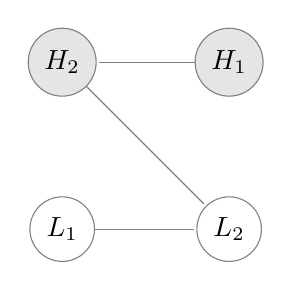
\begin{tikzpicture}[shorten >=1pt,draw=black!50]
	\node (H1) at ( 1.06,  1.06)	[circle, draw, fill = gray!20]	{$H_{1}$};
	\node (H2) at (-1.06,  1.06)	[circle, draw, fill = gray!20]	{$H_{2}$};
	\node (L1) at (-1.06, -1.06)	[circle, draw, fill = white]	{$L_{1}$};
	\node (L2) at ( 1.06, -1.06)	[circle, draw, fill = white]	{$L_{2}$};
	\draw (H1) -- (H2);
	\draw (H2) -- (L2);
	\draw (L1) -- (L2);
\end{tikzpicture}
\end{center}
\columnbreak

\scaleeq{
Equations: \begin{cases}
	e^{H}_{1} \left(\frac{25 \phi}{3} - 3\right) = \alpha + 2 e^{H}_{2} - 2 e^{L}_{1} \theta - 3 e^{L}_{2} \theta - \gamma\\
	e^{H}_{2} \left(\frac{25 \phi}{2} - 2\right) = \alpha + 3 e^{H}_{1} - 2 e^{L}_{1} \theta + 2 e^{L}_{2} \theta - \gamma\\
	e^{L}_{1} \left(\frac{25 \phi}{3 \theta} - 3 \theta\right) = \alpha - 2 e^{H}_{1} - 3 e^{H}_{2} + 2 e^{L}_{2} \theta - \gamma\\
	e^{L}_{2} \left(\frac{25 \phi}{2 \theta} - 2 \theta\right) = \alpha - 2 e^{H}_{1} + 2 e^{H}_{2} + 3 e^{L}_{1} \theta - \gamma
\end{cases}
}\end{multicols}


Optimal efforts:

\scaleeq{
\begin{cases}
	e^{H}_{1} &= \frac{3 \left(\alpha - \gamma\right) \left(125 \phi^{3} - 125 \phi^{2} \theta^{2} + 12 \theta^{4}\right)}{3125 \phi^{4} - 1625 \phi^{3} \theta^{2} - 1625 \phi^{3} + 225 \phi^{2} \theta^{2} + 120 \phi \theta^{4} + 120 \phi \theta^{2} - 36 \theta^{4}}\\
	e^{H}_{2} &= \frac{10 \phi \left(\alpha - \gamma\right) \left(25 \phi^{2} - 15 \phi \theta^{2} - 6 \theta^{2}\right)}{3125 \phi^{4} - 1625 \phi^{3} \theta^{2} - 1625 \phi^{3} + 225 \phi^{2} \theta^{2} + 120 \phi \theta^{4} + 120 \phi \theta^{2} - 36 \theta^{4}}\\
	e^{L}_{1} &= \frac{3 \theta \left(\alpha - \gamma\right) \left(125 \phi^{3} - 125 \phi^{2} + 12 \theta^{2}\right)}{3125 \phi^{4} - 1625 \phi^{3} \theta^{2} - 1625 \phi^{3} + 225 \phi^{2} \theta^{2} + 120 \phi \theta^{4} + 120 \phi \theta^{2} - 36 \theta^{4}}\\
	e^{L}_{2} &= \frac{10 \phi \theta \left(\alpha - \gamma\right) \left(25 \phi^{2} - 15 \phi - 6 \theta^{2}\right)}{3125 \phi^{4} - 1625 \phi^{3} \theta^{2} - 1625 \phi^{3} + 225 \phi^{2} \theta^{2} + 120 \phi \theta^{4} + 120 \phi \theta^{2} - 36 \theta^{4}}
\end{cases}
}

Production Costs:

\scaleeq{
\begin{cases}
	c^{H}_{1} &= - \frac{625 \alpha \phi^{3} - 525 \alpha \phi^{2} \theta^{2} - 60 \alpha \phi \theta^{2} + 36 \alpha \theta^{4} - 3125 \gamma \phi^{4} + 1625 \gamma \phi^{3} \theta^{2} + 1000 \gamma \phi^{3} + 300 \gamma \phi^{2} \theta^{2} - 120 \gamma \phi \theta^{4} - 60 \gamma \phi \theta^{2}}{3125 \phi^{4} - 1625 \phi^{3} \theta^{2} - 1625 \phi^{3} + 225 \phi^{2} \theta^{2} + 120 \phi \theta^{4} + 120 \phi \theta^{2} - 36 \theta^{4}}\\
	c^{H}_{2} &= - \frac{250 \alpha \phi^{3} \theta^{2} + 625 \alpha \phi^{3} - 675 \alpha \phi^{2} \theta^{2} - 60 \alpha \phi \theta^{4} - 60 \alpha \phi \theta^{2} + 36 \alpha \theta^{4} - 3125 \gamma \phi^{4} + 1375 \gamma \phi^{3} \theta^{2} + 1000 \gamma \phi^{3} + 450 \gamma \phi^{2} \theta^{2} - 60 \gamma \phi \theta^{4} - 60 \gamma \phi \theta^{2}}{3125 \phi^{4} - 1625 \phi^{3} \theta^{2} - 1625 \phi^{3} + 225 \phi^{2} \theta^{2} + 120 \phi \theta^{4} + 120 \phi \theta^{2} - 36 \theta^{4}}\\
	c^{L}_{1} &= - \frac{625 \alpha \phi^{3} \theta^{2} - 525 \alpha \phi^{2} \theta^{2} - 60 \alpha \phi \theta^{4} + 36 \alpha \theta^{4} - 3125 \gamma \phi^{4} + 1000 \gamma \phi^{3} \theta^{2} + 1625 \gamma \phi^{3} + 300 \gamma \phi^{2} \theta^{2} - 60 \gamma \phi \theta^{4} - 120 \gamma \phi \theta^{2}}{3125 \phi^{4} - 1625 \phi^{3} \theta^{2} - 1625 \phi^{3} + 225 \phi^{2} \theta^{2} + 120 \phi \theta^{4} + 120 \phi \theta^{2} - 36 \theta^{4}}\\
	c^{L}_{2} &= - \frac{625 \alpha \phi^{3} \theta^{2} + 250 \alpha \phi^{3} - 675 \alpha \phi^{2} \theta^{2} - 60 \alpha \phi \theta^{4} - 60 \alpha \phi \theta^{2} + 36 \alpha \theta^{4} - 3125 \gamma \phi^{4} + 1000 \gamma \phi^{3} \theta^{2} + 1375 \gamma \phi^{3} + 450 \gamma \phi^{2} \theta^{2} - 60 \gamma \phi \theta^{4} - 60 \gamma \phi \theta^{2}}{3125 \phi^{4} - 1625 \phi^{3} \theta^{2} - 1625 \phi^{3} + 225 \phi^{2} \theta^{2} + 120 \phi \theta^{4} + 120 \phi \theta^{2} - 36 \theta^{4}}
\end{cases}
}

Production Quantities:

\scaleeq{
\begin{cases}
	q^{H}_{1} &= \frac{5 \phi \left(\alpha - \gamma\right) \left(125 \phi^{3} - 125 \phi^{2} \theta^{2} + 12 \theta^{4}\right)}{3125 \phi^{4} - 1625 \phi^{3} \theta^{2} - 1625 \phi^{3} + 225 \phi^{2} \theta^{2} + 120 \phi \theta^{4} + 120 \phi \theta^{2} - 36 \theta^{4}}\\
	q^{H}_{2} &= \frac{25 \phi^{2} \left(\alpha - \gamma\right) \left(25 \phi^{2} - 15 \phi \theta^{2} - 6 \theta^{2}\right)}{3125 \phi^{4} - 1625 \phi^{3} \theta^{2} - 1625 \phi^{3} + 225 \phi^{2} \theta^{2} + 120 \phi \theta^{4} + 120 \phi \theta^{2} - 36 \theta^{4}}\\
	q^{L}_{1} &= \frac{5 \phi \left(\alpha - \gamma\right) \left(125 \phi^{3} - 125 \phi^{2} + 12 \theta^{2}\right)}{3125 \phi^{4} - 1625 \phi^{3} \theta^{2} - 1625 \phi^{3} + 225 \phi^{2} \theta^{2} + 120 \phi \theta^{4} + 120 \phi \theta^{2} - 36 \theta^{4}}\\
	q^{L}_{2} &= \frac{25 \phi^{2} \left(\alpha - \gamma\right) \left(25 \phi^{2} - 15 \phi - 6 \theta^{2}\right)}{3125 \phi^{4} - 1625 \phi^{3} \theta^{2} - 1625 \phi^{3} + 225 \phi^{2} \theta^{2} + 120 \phi \theta^{4} + 120 \phi \theta^{2} - 36 \theta^{4}}
\end{cases}
}

Profits:

\begin{equation}
\label{eq:E3E:2H2L_profit}
\scaledequation{\begin{cases}
	\pi^{H}_{1} &= \frac{\phi \left(\alpha - \gamma\right)^{2} \left(25 \phi - 9\right) \left(125 \phi^{3} - 125 \phi^{2} \theta^{2} + 12 \theta^{4}\right)^{2}}{\left(3125 \phi^{4} - 1625 \phi^{3} \theta^{2} - 1625 \phi^{3} + 225 \phi^{2} \theta^{2} + 120 \phi \theta^{4} + 120 \phi \theta^{2} - 36 \theta^{4}\right)^{2}}\\
	\pi^{H}_{2} &= \frac{25 \phi^{3} \left(\alpha - \gamma\right)^{2} \left(25 \phi - 4\right) \left(25 \phi^{2} - 15 \phi \theta^{2} - 6 \theta^{2}\right)^{2}}{\left(3125 \phi^{4} - 1625 \phi^{3} \theta^{2} - 1625 \phi^{3} + 225 \phi^{2} \theta^{2} + 120 \phi \theta^{4} + 120 \phi \theta^{2} - 36 \theta^{4}\right)^{2}}\\
	\pi^{L}_{1} &= \frac{\phi \left(\alpha - \gamma\right)^{2} \left(25 \phi - 9 \theta^{2}\right) \left(125 \phi^{3} - 125 \phi^{2} + 12 \theta^{2}\right)^{2}}{\left(3125 \phi^{4} - 1625 \phi^{3} \theta^{2} - 1625 \phi^{3} + 225 \phi^{2} \theta^{2} + 120 \phi \theta^{4} + 120 \phi \theta^{2} - 36 \theta^{4}\right)^{2}}\\
	\pi^{L}_{2} &= \frac{25 \phi^{3} \left(\alpha - \gamma\right)^{2} \left(25 \phi - 4 \theta^{2}\right) \left(25 \phi^{2} - 15 \phi - 6 \theta^{2}\right)^{2}}{\left(3125 \phi^{4} - 1625 \phi^{3} \theta^{2} - 1625 \phi^{3} + 225 \phi^{2} \theta^{2} + 120 \phi \theta^{4} + 120 \phi \theta^{2} - 36 \theta^{4}\right)^{2}}
\end{cases}
}
\end{equation}

Total Production:

\scaleeq{
\frac{20 \phi \left(\alpha - \gamma\right) \left(125 \phi^{3} - 50 \phi^{2} \theta^{2} - 50 \phi^{2} - 15 \phi \theta^{2} + 3 \theta^{4} + 3 \theta^{2}\right)}{3125 \phi^{4} - 1625 \phi^{3} \theta^{2} - 1625 \phi^{3} + 225 \phi^{2} \theta^{2} + 120 \phi \theta^{4} + 120 \phi \theta^{2} - 36 \theta^{4}}
}

Price:

\scaleeq{
\frac{625 \alpha \phi^{4} - 625 \alpha \phi^{3} \theta^{2} - 625 \alpha \phi^{3} + 525 \alpha \phi^{2} \theta^{2} + 60 \alpha \phi \theta^{4} + 60 \alpha \phi \theta^{2} - 36 \alpha \theta^{4} + 2500 \gamma \phi^{4} - 1000 \gamma \phi^{3} \theta^{2} - 1000 \gamma \phi^{3} - 300 \gamma \phi^{2} \theta^{2} + 60 \gamma \phi \theta^{4} + 60 \gamma \phi \theta^{2}}{3125 \phi^{4} - 1625 \phi^{3} \theta^{2} - 1625 \phi^{3} + 225 \phi^{2} \theta^{2} + 120 \phi \theta^{4} + 120 \phi \theta^{2} - 36 \theta^{4}}
}

Firm Surplus:

\scaleeq{
\frac{\phi \left(\alpha - \gamma\right)^{2} \left(1562500 \phi^{7} - 1453125 \phi^{6} \theta^{2} - 1453125 \phi^{6} + 531250 \phi^{5} \theta^{4} + 337500 \phi^{5} \theta^{2} + 531250 \phi^{5} + 54375 \phi^{4} \theta^{4} + 54375 \phi^{4} \theta^{2} - 75000 \phi^{3} \theta^{6} - 45000 \phi^{3} \theta^{4} - 75000 \phi^{3} \theta^{2} + 23400 \phi^{2} \theta^{6} + 23400 \phi^{2} \theta^{4} + 3600 \phi \theta^{8} + 3600 \phi \theta^{4} - 1296 \theta^{8} - 1296 \theta^{6}\right)}{\left(3125 \phi^{4} - 1625 \phi^{3} \theta^{2} - 1625 \phi^{3} + 225 \phi^{2} \theta^{2} + 120 \phi \theta^{4} + 120 \phi \theta^{2} - 36 \theta^{4}\right)^{2}}
}

Consumer Surplus:

\scaleeq{
\frac{200 \phi^{2} \left(\alpha - \gamma\right)^{2} \left(125 \phi^{3} - 50 \phi^{2} \theta^{2} - 50 \phi^{2} - 15 \phi \theta^{2} + 3 \theta^{4} + 3 \theta^{2}\right)^{2}}{\left(3125 \phi^{4} - 1625 \phi^{3} \theta^{2} - 1625 \phi^{3} + 225 \phi^{2} \theta^{2} + 120 \phi \theta^{4} + 120 \phi \theta^{2} - 36 \theta^{4}\right)^{2}}
}

Social Welfare:

\scaleeq{
\frac{\phi \left(\alpha - \gamma\right)^{2} \left(4687500 \phi^{7} - 3953125 \phi^{6} \theta^{2} - 3953125 \phi^{6} + 1031250 \phi^{5} \theta^{4} + 587500 \phi^{5} \theta^{2} + 1031250 \phi^{5} + 504375 \phi^{4} \theta^{4} + 504375 \phi^{4} \theta^{2} - 135000 \phi^{3} \theta^{6} - 120000 \phi^{3} \theta^{4} - 135000 \phi^{3} \theta^{2} + 5400 \phi^{2} \theta^{6} + 5400 \phi^{2} \theta^{4} + 5400 \phi \theta^{8} + 3600 \phi \theta^{6} + 5400 \phi \theta^{4} - 1296 \theta^{8} - 1296 \theta^{6}\right)}{\left(3125 \phi^{4} - 1625 \phi^{3} \theta^{2} - 1625 \phi^{3} + 225 \phi^{2} \theta^{2} + 120 \phi \theta^{4} + 120 \phi \theta^{2} - 36 \theta^{4}\right)^{2}}
}

%======================================================================

\subsubsection{E3F [2H2L]}
\label{apx:E3F:2H2L}

\begin{multicols}{2}
\begin{center}
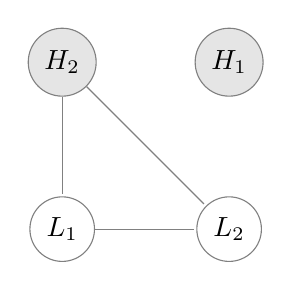
\begin{tikzpicture}[shorten >=1pt,draw=black!50]
	\node (H1) at ( 1.06,  1.06)	[circle, draw, fill = gray!20]	{$H_{1}$};
	\node (H2) at (-1.06,  1.06)	[circle, draw, fill = gray!20]	{$H_{2}$};
	\node (L1) at (-1.06, -1.06)	[circle, draw, fill = white]	{$L_{1}$};
	\node (L2) at ( 1.06, -1.06)	[circle, draw, fill = white]	{$L_{2}$};
	\draw (H2) -- (L1);
	\draw (H2) -- (L2);
	\draw (L1) -- (L2);
\end{tikzpicture}
\end{center}
\columnbreak

\scaleeq{
Equations: \begin{cases}
	e^{H}_{1} \left(\frac{25 \phi}{4} - 4\right) = \alpha - 3 e^{H}_{2} - 3 e^{L}_{1} \theta - 3 e^{L}_{2} \theta - \gamma\\
	e^{H}_{2} \left(\frac{25 \phi}{2} - 2\right) = \alpha - e^{H}_{1} + 2 e^{L}_{1} \theta + 2 e^{L}_{2} \theta - \gamma\\
	e^{L}_{1} \left(\frac{25 \phi}{2 \theta} - 2 \theta\right) = \alpha - e^{H}_{1} + 2 e^{H}_{2} + 2 e^{L}_{2} \theta - \gamma\\
	e^{L}_{2} \left(\frac{25 \phi}{2 \theta} - 2 \theta\right) = \alpha - e^{H}_{1} + 2 e^{H}_{2} + 2 e^{L}_{1} \theta - \gamma
\end{cases}
}\end{multicols}


Optimal efforts:

\scaleeq{
\begin{cases}
	e^{H}_{1} &= \frac{4 \left(\alpha - \gamma\right) \left(5 \phi - 4 \theta^{2} - 2\right)}{125 \phi^{2} - 40 \phi \theta^{2} - 100 \phi + 16 \theta^{2} + 8}\\
	e^{H}_{2} &= \frac{2 \left(\alpha - \gamma\right) \left(5 \phi - 4\right)}{125 \phi^{2} - 40 \phi \theta^{2} - 100 \phi + 16 \theta^{2} + 8}\\
	e^{L}_{1} &= \frac{2 \theta \left(\alpha - \gamma\right) \left(5 \phi - 4\right)}{125 \phi^{2} - 40 \phi \theta^{2} - 100 \phi + 16 \theta^{2} + 8}\\
	e^{L}_{2} &= \frac{2 \theta \left(\alpha - \gamma\right) \left(5 \phi - 4\right)}{125 \phi^{2} - 40 \phi \theta^{2} - 100 \phi + 16 \theta^{2} + 8}
\end{cases}
}

Production Costs:

\scaleeq{
\begin{cases}
	c^{H}_{1} &= - \frac{20 \alpha \phi - 16 \alpha \theta^{2} - 8 \alpha - 125 \gamma \phi^{2} + 40 \gamma \phi \theta^{2} + 80 \gamma \phi}{125 \phi^{2} - 40 \phi \theta^{2} - 100 \phi + 16 \theta^{2} + 8}\\
	c^{H}_{2} &= - \frac{20 \alpha \phi \theta^{2} + 10 \alpha \phi - 16 \alpha \theta^{2} - 8 \alpha - 125 \gamma \phi^{2} + 20 \gamma \phi \theta^{2} + 90 \gamma \phi}{125 \phi^{2} - 40 \phi \theta^{2} - 100 \phi + 16 \theta^{2} + 8}\\
	c^{L}_{1} &= - \frac{20 \alpha \phi \theta^{2} + 10 \alpha \phi - 16 \alpha \theta^{2} - 8 \alpha - 125 \gamma \phi^{2} + 20 \gamma \phi \theta^{2} + 90 \gamma \phi}{125 \phi^{2} - 40 \phi \theta^{2} - 100 \phi + 16 \theta^{2} + 8}\\
	c^{L}_{2} &= - \frac{20 \alpha \phi \theta^{2} + 10 \alpha \phi - 16 \alpha \theta^{2} - 8 \alpha - 125 \gamma \phi^{2} + 20 \gamma \phi \theta^{2} + 90 \gamma \phi}{125 \phi^{2} - 40 \phi \theta^{2} - 100 \phi + 16 \theta^{2} + 8}
\end{cases}
}

Production Quantities:

\scaleeq{
\begin{cases}
	q^{H}_{1} &= \frac{5 \phi \left(\alpha - \gamma\right) \left(5 \phi - 4 \theta^{2} - 2\right)}{125 \phi^{2} - 40 \phi \theta^{2} - 100 \phi + 16 \theta^{2} + 8}\\
	q^{H}_{2} &= \frac{5 \phi \left(\alpha - \gamma\right) \left(5 \phi - 4\right)}{125 \phi^{2} - 40 \phi \theta^{2} - 100 \phi + 16 \theta^{2} + 8}\\
	q^{L}_{1} &= \frac{5 \phi \left(\alpha - \gamma\right) \left(5 \phi - 4\right)}{125 \phi^{2} - 40 \phi \theta^{2} - 100 \phi + 16 \theta^{2} + 8}\\
	q^{L}_{2} &= \frac{5 \phi \left(\alpha - \gamma\right) \left(5 \phi - 4\right)}{125 \phi^{2} - 40 \phi \theta^{2} - 100 \phi + 16 \theta^{2} + 8}
\end{cases}
}

Profits:

\begin{equation}
\label{eq:E3F:2H2L_profit}
\scaledequation{\begin{cases}
	\pi^{H}_{1} &= \frac{\phi \left(\alpha - \gamma\right)^{2} \left(25 \phi - 16\right) \left(5 \phi - 4 \theta^{2} - 2\right)^{2}}{\left(125 \phi^{2} - 40 \phi \theta^{2} - 100 \phi + 16 \theta^{2} + 8\right)^{2}}\\
	\pi^{H}_{2} &= \frac{\phi \left(\alpha - \gamma\right)^{2} \left(5 \phi - 4\right)^{2} \left(25 \phi - 4\right)}{\left(125 \phi^{2} - 40 \phi \theta^{2} - 100 \phi + 16 \theta^{2} + 8\right)^{2}}\\
	\pi^{L}_{1} &= \frac{\phi \left(\alpha - \gamma\right)^{2} \left(5 \phi - 4\right)^{2} \left(25 \phi - 4 \theta^{2}\right)}{\left(125 \phi^{2} - 40 \phi \theta^{2} - 100 \phi + 16 \theta^{2} + 8\right)^{2}}\\
	\pi^{L}_{2} &= \frac{\phi \left(\alpha - \gamma\right)^{2} \left(5 \phi - 4\right)^{2} \left(25 \phi - 4 \theta^{2}\right)}{\left(125 \phi^{2} - 40 \phi \theta^{2} - 100 \phi + 16 \theta^{2} + 8\right)^{2}}
\end{cases}
}
\end{equation}

Total Production:

\scaleeq{
\frac{10 \phi \left(\alpha - \gamma\right) \left(10 \phi - 2 \theta^{2} - 7\right)}{125 \phi^{2} - 40 \phi \theta^{2} - 100 \phi + 16 \theta^{2} + 8}
}

Price:

\scaleeq{
\frac{25 \alpha \phi^{2} - 20 \alpha \phi \theta^{2} - 30 \alpha \phi + 16 \alpha \theta^{2} + 8 \alpha + 100 \gamma \phi^{2} - 20 \gamma \phi \theta^{2} - 70 \gamma \phi}{125 \phi^{2} - 40 \phi \theta^{2} - 100 \phi + 16 \theta^{2} + 8}
}

Firm Surplus:

\scaleeq{
\frac{4 \phi \left(\alpha - \gamma\right)^{2} \left(625 \phi^{3} - 300 \phi^{2} \theta^{2} - 1000 \phi^{2} + 100 \phi \theta^{4} + 340 \phi \theta^{2} + 445 \phi - 64 \theta^{4} - 96 \theta^{2} - 32\right)}{\left(125 \phi^{2} - 40 \phi \theta^{2} - 100 \phi + 16 \theta^{2} + 8\right)^{2}}
}

Consumer Surplus:

\scaleeq{
\frac{50 \phi^{2} \left(\alpha - \gamma\right)^{2} \left(10 \phi - 2 \theta^{2} - 7\right)^{2}}{\left(125 \phi^{2} - 40 \phi \theta^{2} - 100 \phi + 16 \theta^{2} + 8\right)^{2}}
}

Social Welfare:

\scaleeq{
\frac{2 \phi \left(\alpha - \gamma\right)^{2} \left(3750 \phi^{3} - 1600 \phi^{2} \theta^{2} - 5500 \phi^{2} + 300 \phi \theta^{4} + 1380 \phi \theta^{2} + 2115 \phi - 128 \theta^{4} - 192 \theta^{2} - 64\right)}{\left(125 \phi^{2} - 40 \phi \theta^{2} - 100 \phi + 16 \theta^{2} + 8\right)^{2}}
}

%======================================================================

\subsubsection{E3G [2H2L]}
\label{apx:E3G:2H2L}

\begin{multicols}{2}
\begin{center}
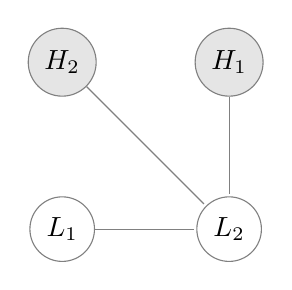
\begin{tikzpicture}[shorten >=1pt,draw=black!50]
	\node (H1) at ( 1.06,  1.06)	[circle, draw, fill = gray!20]	{$H_{1}$};
	\node (H2) at (-1.06,  1.06)	[circle, draw, fill = gray!20]	{$H_{2}$};
	\node (L1) at (-1.06, -1.06)	[circle, draw, fill = white]	{$L_{1}$};
	\node (L2) at ( 1.06, -1.06)	[circle, draw, fill = white]	{$L_{2}$};
	\draw (H1) -- (L2);
	\draw (H2) -- (L2);
	\draw (L1) -- (L2);
\end{tikzpicture}
\end{center}
\columnbreak

\scaleeq{
Equations: \begin{cases}
	e^{H}_{1} \left(\frac{25 \phi}{3} - 3\right) = \alpha - 2 e^{H}_{2} - 2 e^{L}_{1} \theta + e^{L}_{2} \theta - \gamma\\
	e^{H}_{2} \left(\frac{25 \phi}{3} - 3\right) = \alpha - 2 e^{H}_{1} - 2 e^{L}_{1} \theta + e^{L}_{2} \theta - \gamma\\
	e^{L}_{1} \left(\frac{25 \phi}{3 \theta} - 3 \theta\right) = \alpha - 2 e^{H}_{1} - 2 e^{H}_{2} + e^{L}_{2} \theta - \gamma\\
	e^{L}_{2} \left(\frac{25 \phi}{\theta} - \theta\right) = \alpha + 3 e^{H}_{1} + 3 e^{H}_{2} + 3 e^{L}_{1} \theta - \gamma
\end{cases}
}\end{multicols}


Optimal efforts:

\scaleeq{
\begin{cases}
	e^{H}_{1} &= \frac{15 \phi \left(\alpha - \gamma\right) \left(5 \phi - 3 \theta^{2}\right)}{625 \phi^{3} - 250 \phi^{2} \theta^{2} - 75 \phi^{2} - 60 \phi \theta^{2} + 18 \theta^{4}}\\
	e^{H}_{2} &= \frac{15 \phi \left(\alpha - \gamma\right) \left(5 \phi - 3 \theta^{2}\right)}{625 \phi^{3} - 250 \phi^{2} \theta^{2} - 75 \phi^{2} - 60 \phi \theta^{2} + 18 \theta^{4}}\\
	e^{L}_{1} &= \frac{15 \phi \theta \left(\alpha - \gamma\right) \left(5 \phi - 3\right)}{625 \phi^{3} - 250 \phi^{2} \theta^{2} - 75 \phi^{2} - 60 \phi \theta^{2} + 18 \theta^{4}}\\
	e^{L}_{2} &= \frac{\theta \left(\alpha - \gamma\right) \left(25 \phi^{2} + 15 \phi - 18 \theta^{2}\right)}{625 \phi^{3} - 250 \phi^{2} \theta^{2} - 75 \phi^{2} - 60 \phi \theta^{2} + 18 \theta^{4}}
\end{cases}
}

Production Costs:

\scaleeq{
\begin{cases}
	c^{H}_{1} &= - \frac{25 \alpha \phi^{2} \theta^{2} + 75 \alpha \phi^{2} - 30 \alpha \phi \theta^{2} - 18 \alpha \theta^{4} - 625 \gamma \phi^{3} + 225 \gamma \phi^{2} \theta^{2} + 90 \gamma \phi \theta^{2}}{625 \phi^{3} - 250 \phi^{2} \theta^{2} - 75 \phi^{2} - 60 \phi \theta^{2} + 18 \theta^{4}}\\
	c^{H}_{2} &= - \frac{25 \alpha \phi^{2} \theta^{2} + 75 \alpha \phi^{2} - 30 \alpha \phi \theta^{2} - 18 \alpha \theta^{4} - 625 \gamma \phi^{3} + 225 \gamma \phi^{2} \theta^{2} + 90 \gamma \phi \theta^{2}}{625 \phi^{3} - 250 \phi^{2} \theta^{2} - 75 \phi^{2} - 60 \phi \theta^{2} + 18 \theta^{4}}\\
	c^{L}_{1} &= - \frac{100 \alpha \phi^{2} \theta^{2} - 30 \alpha \phi \theta^{2} - 18 \alpha \theta^{4} - 625 \gamma \phi^{3} + 150 \gamma \phi^{2} \theta^{2} + 75 \gamma \phi^{2} + 90 \gamma \phi \theta^{2}}{625 \phi^{3} - 250 \phi^{2} \theta^{2} - 75 \phi^{2} - 60 \phi \theta^{2} + 18 \theta^{4}}\\
	c^{L}_{2} &= - \frac{100 \alpha \phi^{2} \theta^{2} + 150 \alpha \phi^{2} - 120 \alpha \phi \theta^{2} - 18 \alpha \theta^{4} - 625 \gamma \phi^{3} + 150 \gamma \phi^{2} \theta^{2} - 75 \gamma \phi^{2} + 180 \gamma \phi \theta^{2}}{625 \phi^{3} - 250 \phi^{2} \theta^{2} - 75 \phi^{2} - 60 \phi \theta^{2} + 18 \theta^{4}}
\end{cases}
}

Production Quantities:

\scaleeq{
\begin{cases}
	q^{H}_{1} &= \frac{25 \phi^{2} \left(\alpha - \gamma\right) \left(5 \phi - 3 \theta^{2}\right)}{625 \phi^{3} - 250 \phi^{2} \theta^{2} - 75 \phi^{2} - 60 \phi \theta^{2} + 18 \theta^{4}}\\
	q^{H}_{2} &= \frac{25 \phi^{2} \left(\alpha - \gamma\right) \left(5 \phi - 3 \theta^{2}\right)}{625 \phi^{3} - 250 \phi^{2} \theta^{2} - 75 \phi^{2} - 60 \phi \theta^{2} + 18 \theta^{4}}\\
	q^{L}_{1} &= \frac{25 \phi^{2} \left(\alpha - \gamma\right) \left(5 \phi - 3\right)}{625 \phi^{3} - 250 \phi^{2} \theta^{2} - 75 \phi^{2} - 60 \phi \theta^{2} + 18 \theta^{4}}\\
	q^{L}_{2} &= \frac{5 \phi \left(\alpha - \gamma\right) \left(25 \phi^{2} + 15 \phi - 18 \theta^{2}\right)}{625 \phi^{3} - 250 \phi^{2} \theta^{2} - 75 \phi^{2} - 60 \phi \theta^{2} + 18 \theta^{4}}
\end{cases}
}

Profits:

\begin{equation}
\label{eq:E3G:2H2L_profit}
\scaledequation{\begin{cases}
	\pi^{H}_{1} &= \frac{25 \phi^{3} \left(\alpha - \gamma\right)^{2} \left(5 \phi - 3 \theta^{2}\right)^{2} \left(25 \phi - 9\right)}{\left(625 \phi^{3} - 250 \phi^{2} \theta^{2} - 75 \phi^{2} - 60 \phi \theta^{2} + 18 \theta^{4}\right)^{2}}\\
	\pi^{H}_{2} &= \frac{25 \phi^{3} \left(\alpha - \gamma\right)^{2} \left(5 \phi - 3 \theta^{2}\right)^{2} \left(25 \phi - 9\right)}{\left(625 \phi^{3} - 250 \phi^{2} \theta^{2} - 75 \phi^{2} - 60 \phi \theta^{2} + 18 \theta^{4}\right)^{2}}\\
	\pi^{L}_{1} &= \frac{25 \phi^{3} \left(\alpha - \gamma\right)^{2} \left(5 \phi - 3\right)^{2} \left(25 \phi - 9 \theta^{2}\right)}{\left(625 \phi^{3} - 250 \phi^{2} \theta^{2} - 75 \phi^{2} - 60 \phi \theta^{2} + 18 \theta^{4}\right)^{2}}\\
	\pi^{L}_{2} &= \frac{\phi \left(\alpha - \gamma\right)^{2} \left(25 \phi - \theta^{2}\right) \left(25 \phi^{2} + 15 \phi - 18 \theta^{2}\right)^{2}}{\left(625 \phi^{3} - 250 \phi^{2} \theta^{2} - 75 \phi^{2} - 60 \phi \theta^{2} + 18 \theta^{4}\right)^{2}}
\end{cases}
}
\end{equation}

Total Production:

\scaleeq{
\frac{10 \phi \left(\alpha - \gamma\right) \left(50 \phi^{2} - 15 \phi \theta^{2} - 9 \theta^{2}\right)}{625 \phi^{3} - 250 \phi^{2} \theta^{2} - 75 \phi^{2} - 60 \phi \theta^{2} + 18 \theta^{4}}
}

Price:

\scaleeq{
\frac{125 \alpha \phi^{3} - 100 \alpha \phi^{2} \theta^{2} - 75 \alpha \phi^{2} + 30 \alpha \phi \theta^{2} + 18 \alpha \theta^{4} + 500 \gamma \phi^{3} - 150 \gamma \phi^{2} \theta^{2} - 90 \gamma \phi \theta^{2}}{625 \phi^{3} - 250 \phi^{2} \theta^{2} - 75 \phi^{2} - 60 \phi \theta^{2} + 18 \theta^{4}}
}

Firm Surplus:

\scaleeq{
\frac{2 \phi \left(\alpha - \gamma\right)^{2} \left(31250 \phi^{5} - 21875 \phi^{4} \theta^{2} - 5625 \phi^{4} + 5625 \phi^{3} \theta^{4} - 1500 \phi^{3} \theta^{2} + 5625 \phi^{3} - 1575 \phi^{2} \theta^{4} - 7875 \phi^{2} \theta^{2} + 4320 \phi \theta^{4} - 162 \theta^{6}\right)}{\left(625 \phi^{3} - 250 \phi^{2} \theta^{2} - 75 \phi^{2} - 60 \phi \theta^{2} + 18 \theta^{4}\right)^{2}}
}

Consumer Surplus:

\scaleeq{
\frac{50 \phi^{2} \left(\alpha - \gamma\right)^{2} \left(50 \phi^{2} - 15 \phi \theta^{2} - 9 \theta^{2}\right)^{2}}{\left(625 \phi^{3} - 250 \phi^{2} \theta^{2} - 75 \phi^{2} - 60 \phi \theta^{2} + 18 \theta^{4}\right)^{2}}
}

Social Welfare:

\scaleeq{
\frac{2 \phi \left(\alpha - \gamma\right)^{2} \left(93750 \phi^{5} - 59375 \phi^{4} \theta^{2} - 5625 \phi^{4} + 11250 \phi^{3} \theta^{4} - 24000 \phi^{3} \theta^{2} + 5625 \phi^{3} + 5175 \phi^{2} \theta^{4} - 7875 \phi^{2} \theta^{2} + 6345 \phi \theta^{4} - 162 \theta^{6}\right)}{\left(625 \phi^{3} - 250 \phi^{2} \theta^{2} - 75 \phi^{2} - 60 \phi \theta^{2} + 18 \theta^{4}\right)^{2}}
}

%======================================================================

\subsubsection{E3H [2H2L]}
\label{apx:E3H:2H2L}

\begin{multicols}{2}
\begin{center}
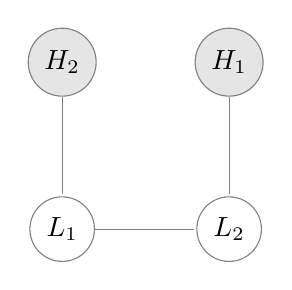
\begin{tikzpicture}[shorten >=1pt,draw=black!50]
	\node (H1) at ( 1.06,  1.06)	[circle, draw, fill = gray!20]	{$H_{1}$};
	\node (H2) at (-1.06,  1.06)	[circle, draw, fill = gray!20]	{$H_{2}$};
	\node (L1) at (-1.06, -1.06)	[circle, draw, fill = white]	{$L_{1}$};
	\node (L2) at ( 1.06, -1.06)	[circle, draw, fill = white]	{$L_{2}$};
	\draw (H1) -- (L2);
	\draw (H2) -- (L1);
	\draw (L1) -- (L2);
\end{tikzpicture}
\end{center}
\columnbreak

\scaleeq{
Equations: \begin{cases}
	e^{H}_{1} \left(\frac{25 \phi}{3} - 3\right) = \alpha - 2 e^{H}_{2} - 3 e^{L}_{1} \theta + 2 e^{L}_{2} \theta - \gamma\\
	e^{H}_{2} \left(\frac{25 \phi}{3} - 3\right) = \alpha - 2 e^{H}_{1} + 2 e^{L}_{1} \theta - 3 e^{L}_{2} \theta - \gamma\\
	e^{L}_{1} \left(\frac{25 \phi}{2 \theta} - 2 \theta\right) = \alpha - 2 e^{H}_{1} + 3 e^{H}_{2} + 2 e^{L}_{2} \theta - \gamma\\
	e^{L}_{2} \left(\frac{25 \phi}{2 \theta} - 2 \theta\right) = \alpha + 3 e^{H}_{1} - 2 e^{H}_{2} + 2 e^{L}_{1} \theta - \gamma
\end{cases}
}\end{multicols}


Optimal efforts:

\scaleeq{
\begin{cases}
	e^{H}_{1} &= \frac{3 \left(\alpha - \gamma\right) \left(5 \phi - 2 \theta^{2}\right)}{125 \phi^{2} - 40 \phi \theta^{2} - 15 \phi + 6 \theta^{2}}\\
	e^{H}_{2} &= \frac{3 \left(\alpha - \gamma\right) \left(5 \phi - 2 \theta^{2}\right)}{125 \phi^{2} - 40 \phi \theta^{2} - 15 \phi + 6 \theta^{2}}\\
	e^{L}_{1} &= \frac{10 \phi \theta \left(\alpha - \gamma\right)}{125 \phi^{2} - 40 \phi \theta^{2} - 15 \phi + 6 \theta^{2}}\\
	e^{L}_{2} &= \frac{10 \phi \theta \left(\alpha - \gamma\right)}{125 \phi^{2} - 40 \phi \theta^{2} - 15 \phi + 6 \theta^{2}}
\end{cases}
}

Production Costs:

\scaleeq{
\begin{cases}
	c^{H}_{1} &= - \frac{10 \alpha \phi \theta^{2} + 15 \alpha \phi - 6 \alpha \theta^{2} - 125 \gamma \phi^{2} + 30 \gamma \phi \theta^{2}}{125 \phi^{2} - 40 \phi \theta^{2} - 15 \phi + 6 \theta^{2}}\\
	c^{H}_{2} &= - \frac{10 \alpha \phi \theta^{2} + 15 \alpha \phi - 6 \alpha \theta^{2} - 125 \gamma \phi^{2} + 30 \gamma \phi \theta^{2}}{125 \phi^{2} - 40 \phi \theta^{2} - 15 \phi + 6 \theta^{2}}\\
	c^{L}_{1} &= - \frac{20 \alpha \phi \theta^{2} + 15 \alpha \phi - 6 \alpha \theta^{2} - 125 \gamma \phi^{2} + 20 \gamma \phi \theta^{2}}{125 \phi^{2} - 40 \phi \theta^{2} - 15 \phi + 6 \theta^{2}}\\
	c^{L}_{2} &= - \frac{20 \alpha \phi \theta^{2} + 15 \alpha \phi - 6 \alpha \theta^{2} - 125 \gamma \phi^{2} + 20 \gamma \phi \theta^{2}}{125 \phi^{2} - 40 \phi \theta^{2} - 15 \phi + 6 \theta^{2}}
\end{cases}
}

Production Quantities:

\scaleeq{
\begin{cases}
	q^{H}_{1} &= \frac{5 \phi \left(\alpha - \gamma\right) \left(5 \phi - 2 \theta^{2}\right)}{125 \phi^{2} - 40 \phi \theta^{2} - 15 \phi + 6 \theta^{2}}\\
	q^{H}_{2} &= \frac{5 \phi \left(\alpha - \gamma\right) \left(5 \phi - 2 \theta^{2}\right)}{125 \phi^{2} - 40 \phi \theta^{2} - 15 \phi + 6 \theta^{2}}\\
	q^{L}_{1} &= \frac{25 \phi^{2} \left(\alpha - \gamma\right)}{125 \phi^{2} - 40 \phi \theta^{2} - 15 \phi + 6 \theta^{2}}\\
	q^{L}_{2} &= \frac{25 \phi^{2} \left(\alpha - \gamma\right)}{125 \phi^{2} - 40 \phi \theta^{2} - 15 \phi + 6 \theta^{2}}
\end{cases}
}

Profits:

\begin{equation}
\label{eq:E3H:2H2L_profit}
\scaledequation{\begin{cases}
	\pi^{H}_{1} &= \frac{\phi \left(\alpha - \gamma\right)^{2} \left(5 \phi - 2 \theta^{2}\right)^{2} \left(25 \phi - 9\right)}{\left(125 \phi^{2} - 40 \phi \theta^{2} - 15 \phi + 6 \theta^{2}\right)^{2}}\\
	\pi^{H}_{2} &= \frac{\phi \left(\alpha - \gamma\right)^{2} \left(5 \phi - 2 \theta^{2}\right)^{2} \left(25 \phi - 9\right)}{\left(125 \phi^{2} - 40 \phi \theta^{2} - 15 \phi + 6 \theta^{2}\right)^{2}}\\
	\pi^{L}_{1} &= \frac{25 \phi^{3} \left(\alpha - \gamma\right)^{2} \left(25 \phi - 4 \theta^{2}\right)}{\left(125 \phi^{2} - 40 \phi \theta^{2} - 15 \phi + 6 \theta^{2}\right)^{2}}\\
	\pi^{L}_{2} &= \frac{25 \phi^{3} \left(\alpha - \gamma\right)^{2} \left(25 \phi - 4 \theta^{2}\right)}{\left(125 \phi^{2} - 40 \phi \theta^{2} - 15 \phi + 6 \theta^{2}\right)^{2}}
\end{cases}
}
\end{equation}

Total Production:

\scaleeq{
\frac{20 \phi \left(\alpha - \gamma\right) \left(5 \phi - \theta^{2}\right)}{125 \phi^{2} - 40 \phi \theta^{2} - 15 \phi + 6 \theta^{2}}
}

Price:

\scaleeq{
\frac{25 \alpha \phi^{2} - 20 \alpha \phi \theta^{2} - 15 \alpha \phi + 6 \alpha \theta^{2} + 100 \gamma \phi^{2} - 20 \gamma \phi \theta^{2}}{125 \phi^{2} - 40 \phi \theta^{2} - 15 \phi + 6 \theta^{2}}
}

Firm Surplus:

\scaleeq{
\frac{2 \phi \left(\alpha - \gamma\right)^{2} \left(1250 \phi^{3} - 600 \phi^{2} \theta^{2} - 225 \phi^{2} + 100 \phi \theta^{4} + 180 \phi \theta^{2} - 36 \theta^{4}\right)}{\left(125 \phi^{2} - 40 \phi \theta^{2} - 15 \phi + 6 \theta^{2}\right)^{2}}
}

Consumer Surplus:

\scaleeq{
\frac{200 \phi^{2} \left(\alpha - \gamma\right)^{2} \left(5 \phi - \theta^{2}\right)^{2}}{\left(125 \phi^{2} - 40 \phi \theta^{2} - 15 \phi + 6 \theta^{2}\right)^{2}}
}

Social Welfare:

\scaleeq{
\frac{2 \phi \left(\alpha - \gamma\right)^{2} \left(3750 \phi^{3} - 1600 \phi^{2} \theta^{2} - 225 \phi^{2} + 200 \phi \theta^{4} + 180 \phi \theta^{2} - 36 \theta^{4}\right)}{\left(125 \phi^{2} - 40 \phi \theta^{2} - 15 \phi + 6 \theta^{2}\right)^{2}}
}

%======================================================================

\subsubsection{E4A [2H2L]}
\label{apx:E4A:2H2L}

\begin{multicols}{2}
\begin{center}
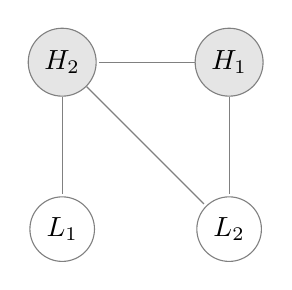
\begin{tikzpicture}[shorten >=1pt,draw=black!50]
	\node (H1) at ( 1.06,  1.06)	[circle, draw, fill = gray!20]	{$H_{1}$};
	\node (H2) at (-1.06,  1.06)	[circle, draw, fill = gray!20]	{$H_{2}$};
	\node (L1) at (-1.06, -1.06)	[circle, draw, fill = white]	{$L_{1}$};
	\node (L2) at ( 1.06, -1.06)	[circle, draw, fill = white]	{$L_{2}$};
	\draw (H1) -- (H2);
	\draw (H1) -- (L2);
	\draw (H2) -- (L1);
	\draw (H2) -- (L2);
\end{tikzpicture}
\end{center}
\columnbreak

\scaleeq{
Equations: \begin{cases}
	e^{H}_{1} \left(\frac{25 \phi}{2} - 2\right) = \alpha + e^{H}_{2} - 2 e^{L}_{1} \theta + 2 e^{L}_{2} \theta - \gamma\\
	e^{H}_{2} \left(25 \phi - 1\right) = \alpha + 2 e^{H}_{1} + 3 e^{L}_{1} \theta + 2 e^{L}_{2} \theta - \gamma\\
	e^{L}_{1} \left(\frac{25 \phi}{3 \theta} - 3 \theta\right) = \alpha - 3 e^{H}_{1} + e^{H}_{2} - 3 e^{L}_{2} \theta - \gamma\\
	e^{L}_{2} \left(\frac{25 \phi}{2 \theta} - 2 \theta\right) = \alpha + 2 e^{H}_{1} + e^{H}_{2} - 2 e^{L}_{1} \theta - \gamma
\end{cases}
}\end{multicols}


Optimal efforts:

\scaleeq{
\begin{cases}
	e^{H}_{1} &= \frac{10 \phi \left(\alpha - \gamma\right) \left(5 \phi - 3 \theta^{2}\right)}{625 \phi^{3} - 325 \phi^{2} \theta^{2} - 125 \phi^{2} + 6 \theta^{4} + 6 \theta^{2}}\\
	e^{H}_{2} &= \frac{\left(\alpha - \gamma\right) \left(25 \phi^{2} - 6 \theta^{4} - 6 \theta^{2}\right)}{625 \phi^{3} - 325 \phi^{2} \theta^{2} - 125 \phi^{2} + 6 \theta^{4} + 6 \theta^{2}}\\
	e^{L}_{1} &= \frac{15 \phi \theta \left(\alpha - \gamma\right) \left(5 \phi - 2 \theta^{2} - 2\right)}{625 \phi^{3} - 325 \phi^{2} \theta^{2} - 125 \phi^{2} + 6 \theta^{4} + 6 \theta^{2}}\\
	e^{L}_{2} &= \frac{10 \phi \theta \left(\alpha - \gamma\right) \left(5 \phi - 3 \theta^{2}\right)}{625 \phi^{3} - 325 \phi^{2} \theta^{2} - 125 \phi^{2} + 6 \theta^{4} + 6 \theta^{2}}
\end{cases}
}

Production Costs:

\scaleeq{
\begin{cases}
	c^{H}_{1} &= - \frac{50 \alpha \phi^{2} \theta^{2} + 75 \alpha \phi^{2} - 30 \alpha \phi \theta^{4} - 30 \alpha \phi \theta^{2} - 6 \alpha \theta^{4} - 6 \alpha \theta^{2} - 625 \gamma \phi^{3} + 275 \gamma \phi^{2} \theta^{2} + 50 \gamma \phi^{2} + 30 \gamma \phi \theta^{4} + 30 \gamma \phi \theta^{2}}{625 \phi^{3} - 325 \phi^{2} \theta^{2} - 125 \phi^{2} + 6 \theta^{4} + 6 \theta^{2}}\\
	c^{H}_{2} &= - \frac{125 \alpha \phi^{2} \theta^{2} + 75 \alpha \phi^{2} - 60 \alpha \phi \theta^{4} - 60 \alpha \phi \theta^{2} - 6 \alpha \theta^{4} - 6 \alpha \theta^{2} - 625 \gamma \phi^{3} + 200 \gamma \phi^{2} \theta^{2} + 50 \gamma \phi^{2} + 60 \gamma \phi \theta^{4} + 60 \gamma \phi \theta^{2}}{625 \phi^{3} - 325 \phi^{2} \theta^{2} - 125 \phi^{2} + 6 \theta^{4} + 6 \theta^{2}}\\
	c^{L}_{1} &= - \frac{75 \alpha \phi^{2} \theta^{2} + 25 \alpha \phi^{2} - 30 \alpha \phi \theta^{4} - 30 \alpha \phi \theta^{2} - 6 \alpha \theta^{4} - 6 \alpha \theta^{2} - 625 \gamma \phi^{3} + 250 \gamma \phi^{2} \theta^{2} + 100 \gamma \phi^{2} + 30 \gamma \phi \theta^{4} + 30 \gamma \phi \theta^{2}}{625 \phi^{3} - 325 \phi^{2} \theta^{2} - 125 \phi^{2} + 6 \theta^{4} + 6 \theta^{2}}\\
	c^{L}_{2} &= - \frac{50 \alpha \phi^{2} \theta^{2} + 75 \alpha \phi^{2} - 30 \alpha \phi \theta^{4} - 30 \alpha \phi \theta^{2} - 6 \alpha \theta^{4} - 6 \alpha \theta^{2} - 625 \gamma \phi^{3} + 275 \gamma \phi^{2} \theta^{2} + 50 \gamma \phi^{2} + 30 \gamma \phi \theta^{4} + 30 \gamma \phi \theta^{2}}{625 \phi^{3} - 325 \phi^{2} \theta^{2} - 125 \phi^{2} + 6 \theta^{4} + 6 \theta^{2}}
\end{cases}
}

Production Quantities:

\scaleeq{
\begin{cases}
	q^{H}_{1} &= \frac{25 \phi^{2} \left(\alpha - \gamma\right) \left(5 \phi - 3 \theta^{2}\right)}{625 \phi^{3} - 325 \phi^{2} \theta^{2} - 125 \phi^{2} + 6 \theta^{4} + 6 \theta^{2}}\\
	q^{H}_{2} &= \frac{5 \phi \left(\alpha - \gamma\right) \left(25 \phi^{2} - 6 \theta^{4} - 6 \theta^{2}\right)}{625 \phi^{3} - 325 \phi^{2} \theta^{2} - 125 \phi^{2} + 6 \theta^{4} + 6 \theta^{2}}\\
	q^{L}_{1} &= \frac{25 \phi^{2} \left(\alpha - \gamma\right) \left(5 \phi - 2 \theta^{2} - 2\right)}{625 \phi^{3} - 325 \phi^{2} \theta^{2} - 125 \phi^{2} + 6 \theta^{4} + 6 \theta^{2}}\\
	q^{L}_{2} &= \frac{25 \phi^{2} \left(\alpha - \gamma\right) \left(5 \phi - 3 \theta^{2}\right)}{625 \phi^{3} - 325 \phi^{2} \theta^{2} - 125 \phi^{2} + 6 \theta^{4} + 6 \theta^{2}}
\end{cases}
}

Profits:

\begin{equation}
\label{eq:E4A:2H2L_profit}
\scaledequation{\begin{cases}
	\pi^{H}_{1} &= \frac{25 \phi^{3} \left(\alpha - \gamma\right)^{2} \left(5 \phi - 3 \theta^{2}\right)^{2} \left(25 \phi - 4\right)}{\left(625 \phi^{3} - 325 \phi^{2} \theta^{2} - 125 \phi^{2} + 6 \theta^{4} + 6 \theta^{2}\right)^{2}}\\
	\pi^{H}_{2} &= \frac{\phi \left(\alpha - \gamma\right)^{2} \left(25 \phi - 1\right) \left(25 \phi^{2} - 6 \theta^{4} - 6 \theta^{2}\right)^{2}}{\left(625 \phi^{3} - 325 \phi^{2} \theta^{2} - 125 \phi^{2} + 6 \theta^{4} + 6 \theta^{2}\right)^{2}}\\
	\pi^{L}_{1} &= \frac{25 \phi^{3} \left(\alpha - \gamma\right)^{2} \left(25 \phi - 9 \theta^{2}\right) \left(5 \phi - 2 \theta^{2} - 2\right)^{2}}{\left(625 \phi^{3} - 325 \phi^{2} \theta^{2} - 125 \phi^{2} + 6 \theta^{4} + 6 \theta^{2}\right)^{2}}\\
	\pi^{L}_{2} &= \frac{25 \phi^{3} \left(\alpha - \gamma\right)^{2} \left(5 \phi - 3 \theta^{2}\right)^{2} \left(25 \phi - 4 \theta^{2}\right)}{\left(625 \phi^{3} - 325 \phi^{2} \theta^{2} - 125 \phi^{2} + 6 \theta^{4} + 6 \theta^{2}\right)^{2}}
\end{cases}
}
\end{equation}

Total Production:

\scaleeq{
\frac{10 \phi \left(\alpha - \gamma\right) \left(50 \phi^{2} - 20 \phi \theta^{2} - 5 \phi - 3 \theta^{4} - 3 \theta^{2}\right)}{625 \phi^{3} - 325 \phi^{2} \theta^{2} - 125 \phi^{2} + 6 \theta^{4} + 6 \theta^{2}}
}

Price:

\scaleeq{
\frac{125 \alpha \phi^{3} - 125 \alpha \phi^{2} \theta^{2} - 75 \alpha \phi^{2} + 30 \alpha \phi \theta^{4} + 30 \alpha \phi \theta^{2} + 6 \alpha \theta^{4} + 6 \alpha \theta^{2} + 500 \gamma \phi^{3} - 200 \gamma \phi^{2} \theta^{2} - 50 \gamma \phi^{2} - 30 \gamma \phi \theta^{4} - 30 \gamma \phi \theta^{2}}{625 \phi^{3} - 325 \phi^{2} \theta^{2} - 125 \phi^{2} + 6 \theta^{4} + 6 \theta^{2}}
}

Firm Surplus:

\scaleeq{
\frac{\phi \left(\alpha - \gamma\right)^{2} \left(62500 \phi^{5} - 58125 \phi^{4} \theta^{2} - 15625 \phi^{4} + 13750 \phi^{3} \theta^{4} + 5000 \phi^{3} \theta^{2} + 2500 \phi^{3} - 1800 \phi^{2} \theta^{6} - 2400 \phi^{2} \theta^{4} - 600 \phi^{2} \theta^{2} + 900 \phi \theta^{8} + 1800 \phi \theta^{6} + 900 \phi \theta^{4} - 36 \theta^{8} - 72 \theta^{6} - 36 \theta^{4}\right)}{\left(625 \phi^{3} - 325 \phi^{2} \theta^{2} - 125 \phi^{2} + 6 \theta^{4} + 6 \theta^{2}\right)^{2}}
}

Consumer Surplus:

\scaleeq{
\frac{50 \phi^{2} \left(\alpha - \gamma\right)^{2} \left(50 \phi^{2} - 20 \phi \theta^{2} - 5 \phi - 3 \theta^{4} - 3 \theta^{2}\right)^{2}}{\left(625 \phi^{3} - 325 \phi^{2} \theta^{2} - 125 \phi^{2} + 6 \theta^{4} + 6 \theta^{2}\right)^{2}}
}

Social Welfare:

\scaleeq{
\frac{\phi \left(\alpha - \gamma\right)^{2} \left(187500 \phi^{5} - 158125 \phi^{4} \theta^{2} - 40625 \phi^{4} + 18750 \phi^{3} \theta^{4} + 3750 \phi^{3} + 4200 \phi^{2} \theta^{6} + 5100 \phi^{2} \theta^{4} + 900 \phi^{2} \theta^{2} + 1350 \phi \theta^{8} + 2700 \phi \theta^{6} + 1350 \phi \theta^{4} - 36 \theta^{8} - 72 \theta^{6} - 36 \theta^{4}\right)}{\left(625 \phi^{3} - 325 \phi^{2} \theta^{2} - 125 \phi^{2} + 6 \theta^{4} + 6 \theta^{2}\right)^{2}}
}

%======================================================================

\subsubsection{E4B [2H2L]}
\label{apx:E4B:2H2L}

\begin{multicols}{2}
\begin{center}
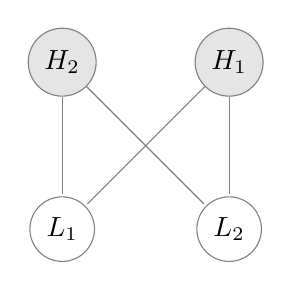
\begin{tikzpicture}[shorten >=1pt,draw=black!50]
	\node (H1) at ( 1.06,  1.06)	[circle, draw, fill = gray!20]	{$H_{1}$};
	\node (H2) at (-1.06,  1.06)	[circle, draw, fill = gray!20]	{$H_{2}$};
	\node (L1) at (-1.06, -1.06)	[circle, draw, fill = white]	{$L_{1}$};
	\node (L2) at ( 1.06, -1.06)	[circle, draw, fill = white]	{$L_{2}$};
	\draw (H1) -- (L1);
	\draw (H1) -- (L2);
	\draw (H2) -- (L1);
	\draw (H2) -- (L2);
\end{tikzpicture}
\end{center}
\columnbreak

\scaleeq{
Equations: \begin{cases}
	e^{H}_{1} \left(\frac{25 \phi}{2} - 2\right) = \alpha - 3 e^{H}_{2} + 2 e^{L}_{1} \theta + 2 e^{L}_{2} \theta - \gamma\\
	e^{H}_{2} \left(\frac{25 \phi}{2} - 2\right) = \alpha - 3 e^{H}_{1} + 2 e^{L}_{1} \theta + 2 e^{L}_{2} \theta - \gamma\\
	e^{L}_{1} \left(\frac{25 \phi}{2 \theta} - 2 \theta\right) = \alpha + 2 e^{H}_{1} + 2 e^{H}_{2} - 3 e^{L}_{2} \theta - \gamma\\
	e^{L}_{2} \left(\frac{25 \phi}{2 \theta} - 2 \theta\right) = \alpha + 2 e^{H}_{1} + 2 e^{H}_{2} - 3 e^{L}_{1} \theta - \gamma
\end{cases}
}\end{multicols}


Optimal efforts:

\scaleeq{
\begin{cases}
	e^{H}_{1} &= \frac{2 \left(\alpha - \gamma\right) \left(5 \phi + 2 \theta^{2}\right)}{125 \phi^{2} + 10 \phi \theta^{2} + 10 \phi - 12 \theta^{2}}\\
	e^{H}_{2} &= \frac{2 \left(\alpha - \gamma\right) \left(5 \phi + 2 \theta^{2}\right)}{125 \phi^{2} + 10 \phi \theta^{2} + 10 \phi - 12 \theta^{2}}\\
	e^{L}_{1} &= \frac{2 \theta \left(\alpha - \gamma\right) \left(5 \phi + 2\right)}{125 \phi^{2} + 10 \phi \theta^{2} + 10 \phi - 12 \theta^{2}}\\
	e^{L}_{2} &= \frac{2 \theta \left(\alpha - \gamma\right) \left(5 \phi + 2\right)}{125 \phi^{2} + 10 \phi \theta^{2} + 10 \phi - 12 \theta^{2}}
\end{cases}
}

Production Costs:

\scaleeq{
\begin{cases}
	c^{H}_{1} &= - \frac{20 \alpha \phi \theta^{2} + 10 \alpha \phi + 12 \alpha \theta^{2} - 125 \gamma \phi^{2} - 30 \gamma \phi \theta^{2} - 20 \gamma \phi}{125 \phi^{2} + 10 \phi \theta^{2} + 10 \phi - 12 \theta^{2}}\\
	c^{H}_{2} &= - \frac{20 \alpha \phi \theta^{2} + 10 \alpha \phi + 12 \alpha \theta^{2} - 125 \gamma \phi^{2} - 30 \gamma \phi \theta^{2} - 20 \gamma \phi}{125 \phi^{2} + 10 \phi \theta^{2} + 10 \phi - 12 \theta^{2}}\\
	c^{L}_{1} &= - \frac{10 \alpha \phi \theta^{2} + 20 \alpha \phi + 12 \alpha \theta^{2} - 125 \gamma \phi^{2} - 20 \gamma \phi \theta^{2} - 30 \gamma \phi}{125 \phi^{2} + 10 \phi \theta^{2} + 10 \phi - 12 \theta^{2}}\\
	c^{L}_{2} &= - \frac{10 \alpha \phi \theta^{2} + 20 \alpha \phi + 12 \alpha \theta^{2} - 125 \gamma \phi^{2} - 20 \gamma \phi \theta^{2} - 30 \gamma \phi}{125 \phi^{2} + 10 \phi \theta^{2} + 10 \phi - 12 \theta^{2}}
\end{cases}
}

Production Quantities:

\scaleeq{
\begin{cases}
	q^{H}_{1} &= \frac{5 \phi \left(\alpha - \gamma\right) \left(5 \phi + 2 \theta^{2}\right)}{125 \phi^{2} + 10 \phi \theta^{2} + 10 \phi - 12 \theta^{2}}\\
	q^{H}_{2} &= \frac{5 \phi \left(\alpha - \gamma\right) \left(5 \phi + 2 \theta^{2}\right)}{125 \phi^{2} + 10 \phi \theta^{2} + 10 \phi - 12 \theta^{2}}\\
	q^{L}_{1} &= \frac{5 \phi \left(\alpha - \gamma\right) \left(5 \phi + 2\right)}{125 \phi^{2} + 10 \phi \theta^{2} + 10 \phi - 12 \theta^{2}}\\
	q^{L}_{2} &= \frac{5 \phi \left(\alpha - \gamma\right) \left(5 \phi + 2\right)}{125 \phi^{2} + 10 \phi \theta^{2} + 10 \phi - 12 \theta^{2}}
\end{cases}
}

Profits:

\begin{equation}
\label{eq:E4B:2H2L_profit}
\scaledequation{\begin{cases}
	\pi^{H}_{1} &= \frac{\phi \left(\alpha - \gamma\right)^{2} \left(5 \phi + 2 \theta^{2}\right)^{2} \left(25 \phi - 4\right)}{\left(125 \phi^{2} + 10 \phi \theta^{2} + 10 \phi - 12 \theta^{2}\right)^{2}}\\
	\pi^{H}_{2} &= \frac{\phi \left(\alpha - \gamma\right)^{2} \left(5 \phi + 2 \theta^{2}\right)^{2} \left(25 \phi - 4\right)}{\left(125 \phi^{2} + 10 \phi \theta^{2} + 10 \phi - 12 \theta^{2}\right)^{2}}\\
	\pi^{L}_{1} &= \frac{\phi \left(\alpha - \gamma\right)^{2} \left(5 \phi + 2\right)^{2} \left(25 \phi - 4 \theta^{2}\right)}{\left(125 \phi^{2} + 10 \phi \theta^{2} + 10 \phi - 12 \theta^{2}\right)^{2}}\\
	\pi^{L}_{2} &= \frac{\phi \left(\alpha - \gamma\right)^{2} \left(5 \phi + 2\right)^{2} \left(25 \phi - 4 \theta^{2}\right)}{\left(125 \phi^{2} + 10 \phi \theta^{2} + 10 \phi - 12 \theta^{2}\right)^{2}}
\end{cases}
}
\end{equation}

Total Production:

\scaleeq{
\frac{20 \phi \left(\alpha - \gamma\right) \left(5 \phi + \theta^{2} + 1\right)}{125 \phi^{2} + 10 \phi \theta^{2} + 10 \phi - 12 \theta^{2}}
}

Price:

\scaleeq{
\frac{25 \alpha \phi^{2} - 10 \alpha \phi \theta^{2} - 10 \alpha \phi - 12 \alpha \theta^{2} + 100 \gamma \phi^{2} + 20 \gamma \phi \theta^{2} + 20 \gamma \phi}{125 \phi^{2} + 10 \phi \theta^{2} + 10 \phi - 12 \theta^{2}}
}

Firm Surplus:

\scaleeq{
\frac{4 \phi \left(\alpha - \gamma\right)^{2} \left(625 \phi^{3} + 200 \phi^{2} \theta^{2} + 200 \phi^{2} + 50 \phi \theta^{4} - 80 \phi \theta^{2} + 50 \phi - 8 \theta^{4} - 8 \theta^{2}\right)}{\left(125 \phi^{2} + 10 \phi \theta^{2} + 10 \phi - 12 \theta^{2}\right)^{2}}
}

Consumer Surplus:

\scaleeq{
\frac{200 \phi^{2} \left(\alpha - \gamma\right)^{2} \left(5 \phi + \theta^{2} + 1\right)^{2}}{\left(125 \phi^{2} + 10 \phi \theta^{2} + 10 \phi - 12 \theta^{2}\right)^{2}}
}

Social Welfare:

\scaleeq{
\frac{4 \phi \left(\alpha - \gamma\right)^{2} \left(1875 \phi^{3} + 700 \phi^{2} \theta^{2} + 700 \phi^{2} + 100 \phi \theta^{4} + 20 \phi \theta^{2} + 100 \phi - 8 \theta^{4} - 8 \theta^{2}\right)}{\left(125 \phi^{2} + 10 \phi \theta^{2} + 10 \phi - 12 \theta^{2}\right)^{2}}
}

%======================================================================

\subsubsection{E4C [2H2L]}
\label{apx:E4C:2H2L}

\begin{multicols}{2}
\begin{center}
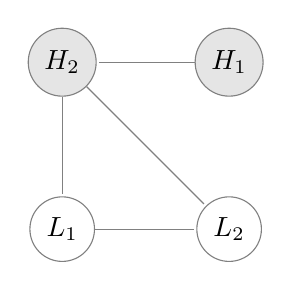
\begin{tikzpicture}[shorten >=1pt,draw=black!50]
	\node (H1) at ( 1.06,  1.06)	[circle, draw, fill = gray!20]	{$H_{1}$};
	\node (H2) at (-1.06,  1.06)	[circle, draw, fill = gray!20]	{$H_{2}$};
	\node (L1) at (-1.06, -1.06)	[circle, draw, fill = white]	{$L_{1}$};
	\node (L2) at ( 1.06, -1.06)	[circle, draw, fill = white]	{$L_{2}$};
	\draw (H1) -- (H2);
	\draw (H2) -- (L1);
	\draw (H2) -- (L2);
	\draw (L1) -- (L2);
\end{tikzpicture}
\end{center}
\columnbreak

\scaleeq{
Equations: \begin{cases}
	e^{H}_{1} \left(\frac{25 \phi}{3} - 3\right) = \alpha + e^{H}_{2} - 3 e^{L}_{1} \theta - 3 e^{L}_{2} \theta - \gamma\\
	e^{H}_{2} \left(25 \phi - 1\right) = \alpha + 3 e^{H}_{1} + 2 e^{L}_{1} \theta + 2 e^{L}_{2} \theta - \gamma\\
	e^{L}_{1} \left(\frac{25 \phi}{2 \theta} - 2 \theta\right) = \alpha - 2 e^{H}_{1} + e^{H}_{2} + 2 e^{L}_{2} \theta - \gamma\\
	e^{L}_{2} \left(\frac{25 \phi}{2 \theta} - 2 \theta\right) = \alpha - 2 e^{H}_{1} + e^{H}_{2} + 2 e^{L}_{1} \theta - \gamma
\end{cases}
}\end{multicols}


Optimal efforts:

\scaleeq{
\begin{cases}
	e^{H}_{1} &= \frac{15 \phi \left(\alpha - \gamma\right) \left(5 \phi - 4 \theta^{2}\right)}{625 \phi^{3} - 200 \phi^{2} \theta^{2} - 250 \phi^{2} + 12 \theta^{2}}\\
	e^{H}_{2} &= \frac{\left(\alpha - \gamma\right) \left(25 \phi^{2} - 12 \theta^{2}\right)}{625 \phi^{3} - 200 \phi^{2} \theta^{2} - 250 \phi^{2} + 12 \theta^{2}}\\
	e^{L}_{1} &= \frac{10 \phi \theta \left(\alpha - \gamma\right) \left(5 \phi - 3\right)}{625 \phi^{3} - 200 \phi^{2} \theta^{2} - 250 \phi^{2} + 12 \theta^{2}}\\
	e^{L}_{2} &= \frac{10 \phi \theta \left(\alpha - \gamma\right) \left(5 \phi - 3\right)}{625 \phi^{3} - 200 \phi^{2} \theta^{2} - 250 \phi^{2} + 12 \theta^{2}}
\end{cases}
}

Production Costs:

\scaleeq{
\begin{cases}
	c^{H}_{1} &= - \frac{100 \alpha \phi^{2} - 60 \alpha \phi \theta^{2} - 12 \alpha \theta^{2} - 625 \gamma \phi^{3} + 200 \gamma \phi^{2} \theta^{2} + 150 \gamma \phi^{2} + 60 \gamma \phi \theta^{2}}{625 \phi^{3} - 200 \phi^{2} \theta^{2} - 250 \phi^{2} + 12 \theta^{2}}\\
	c^{H}_{2} &= - \frac{100 \alpha \phi^{2} \theta^{2} + 100 \alpha \phi^{2} - 120 \alpha \phi \theta^{2} - 12 \alpha \theta^{2} - 625 \gamma \phi^{3} + 100 \gamma \phi^{2} \theta^{2} + 150 \gamma \phi^{2} + 120 \gamma \phi \theta^{2}}{625 \phi^{3} - 200 \phi^{2} \theta^{2} - 250 \phi^{2} + 12 \theta^{2}}\\
	c^{L}_{1} &= - \frac{100 \alpha \phi^{2} \theta^{2} + 25 \alpha \phi^{2} - 60 \alpha \phi \theta^{2} - 12 \alpha \theta^{2} - 625 \gamma \phi^{3} + 100 \gamma \phi^{2} \theta^{2} + 225 \gamma \phi^{2} + 60 \gamma \phi \theta^{2}}{625 \phi^{3} - 200 \phi^{2} \theta^{2} - 250 \phi^{2} + 12 \theta^{2}}\\
	c^{L}_{2} &= - \frac{100 \alpha \phi^{2} \theta^{2} + 25 \alpha \phi^{2} - 60 \alpha \phi \theta^{2} - 12 \alpha \theta^{2} - 625 \gamma \phi^{3} + 100 \gamma \phi^{2} \theta^{2} + 225 \gamma \phi^{2} + 60 \gamma \phi \theta^{2}}{625 \phi^{3} - 200 \phi^{2} \theta^{2} - 250 \phi^{2} + 12 \theta^{2}}
\end{cases}
}

Production Quantities:

\scaleeq{
\begin{cases}
	q^{H}_{1} &= \frac{25 \phi^{2} \left(\alpha - \gamma\right) \left(5 \phi - 4 \theta^{2}\right)}{625 \phi^{3} - 200 \phi^{2} \theta^{2} - 250 \phi^{2} + 12 \theta^{2}}\\
	q^{H}_{2} &= \frac{5 \phi \left(\alpha - \gamma\right) \left(25 \phi^{2} - 12 \theta^{2}\right)}{625 \phi^{3} - 200 \phi^{2} \theta^{2} - 250 \phi^{2} + 12 \theta^{2}}\\
	q^{L}_{1} &= \frac{25 \phi^{2} \left(\alpha - \gamma\right) \left(5 \phi - 3\right)}{625 \phi^{3} - 200 \phi^{2} \theta^{2} - 250 \phi^{2} + 12 \theta^{2}}\\
	q^{L}_{2} &= \frac{25 \phi^{2} \left(\alpha - \gamma\right) \left(5 \phi - 3\right)}{625 \phi^{3} - 200 \phi^{2} \theta^{2} - 250 \phi^{2} + 12 \theta^{2}}
\end{cases}
}

Profits:

\begin{equation}
\label{eq:E4C:2H2L_profit}
\scaledequation{\begin{cases}
	\pi^{H}_{1} &= \frac{25 \phi^{3} \left(\alpha - \gamma\right)^{2} \left(5 \phi - 4 \theta^{2}\right)^{2} \left(25 \phi - 9\right)}{\left(625 \phi^{3} - 200 \phi^{2} \theta^{2} - 250 \phi^{2} + 12 \theta^{2}\right)^{2}}\\
	\pi^{H}_{2} &= \frac{\phi \left(\alpha - \gamma\right)^{2} \left(25 \phi - 1\right) \left(25 \phi^{2} - 12 \theta^{2}\right)^{2}}{\left(625 \phi^{3} - 200 \phi^{2} \theta^{2} - 250 \phi^{2} + 12 \theta^{2}\right)^{2}}\\
	\pi^{L}_{1} &= \frac{25 \phi^{3} \left(\alpha - \gamma\right)^{2} \left(5 \phi - 3\right)^{2} \left(25 \phi - 4 \theta^{2}\right)}{\left(625 \phi^{3} - 200 \phi^{2} \theta^{2} - 250 \phi^{2} + 12 \theta^{2}\right)^{2}}\\
	\pi^{L}_{2} &= \frac{25 \phi^{3} \left(\alpha - \gamma\right)^{2} \left(5 \phi - 3\right)^{2} \left(25 \phi - 4 \theta^{2}\right)}{\left(625 \phi^{3} - 200 \phi^{2} \theta^{2} - 250 \phi^{2} + 12 \theta^{2}\right)^{2}}
\end{cases}
}
\end{equation}

Total Production:

\scaleeq{
\frac{10 \phi \left(\alpha - \gamma\right) \left(50 \phi^{2} - 10 \phi \theta^{2} - 15 \phi - 6 \theta^{2}\right)}{625 \phi^{3} - 200 \phi^{2} \theta^{2} - 250 \phi^{2} + 12 \theta^{2}}
}

Price:

\scaleeq{
\frac{125 \alpha \phi^{3} - 100 \alpha \phi^{2} \theta^{2} - 100 \alpha \phi^{2} + 60 \alpha \phi \theta^{2} + 12 \alpha \theta^{2} + 500 \gamma \phi^{3} - 100 \gamma \phi^{2} \theta^{2} - 150 \gamma \phi^{2} - 60 \gamma \phi \theta^{2}}{625 \phi^{3} - 200 \phi^{2} \theta^{2} - 250 \phi^{2} + 12 \theta^{2}}
}

Firm Surplus:

\scaleeq{
\frac{2 \phi \left(\alpha - \gamma\right)^{2} \left(31250 \phi^{5} - 15000 \phi^{4} \theta^{2} - 21875 \phi^{4} + 5000 \phi^{3} \theta^{4} + 5625 \phi^{3} - 1800 \phi^{2} \theta^{4} - 600 \phi^{2} \theta^{2} + 1800 \phi \theta^{4} - 72 \theta^{4}\right)}{\left(625 \phi^{3} - 200 \phi^{2} \theta^{2} - 250 \phi^{2} + 12 \theta^{2}\right)^{2}}
}

Consumer Surplus:

\scaleeq{
\frac{50 \phi^{2} \left(\alpha - \gamma\right)^{2} \left(50 \phi^{2} - 10 \phi \theta^{2} - 15 \phi - 6 \theta^{2}\right)^{2}}{\left(625 \phi^{3} - 200 \phi^{2} \theta^{2} - 250 \phi^{2} + 12 \theta^{2}\right)^{2}}
}

Social Welfare:

\scaleeq{
\frac{2 \phi \left(\alpha - \gamma\right)^{2} \left(93750 \phi^{5} - 40000 \phi^{4} \theta^{2} - 59375 \phi^{4} + 7500 \phi^{3} \theta^{4} - 7500 \phi^{3} \theta^{2} + 11250 \phi^{3} + 1200 \phi^{2} \theta^{4} + 3900 \phi^{2} \theta^{2} + 2700 \phi \theta^{4} - 72 \theta^{4}\right)}{\left(625 \phi^{3} - 200 \phi^{2} \theta^{2} - 250 \phi^{2} + 12 \theta^{2}\right)^{2}}
}

%======================================================================

\subsubsection{E4D [2H2L]}
\label{apx:E4D:2H2L}

\begin{multicols}{2}
\begin{center}
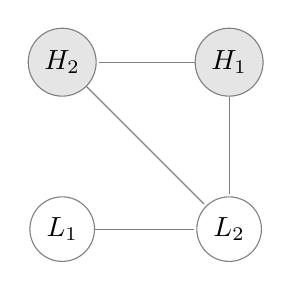
\begin{tikzpicture}[shorten >=1pt,draw=black!50]
	\node (H1) at ( 1.06,  1.06)	[circle, draw, fill = gray!20]	{$H_{1}$};
	\node (H2) at (-1.06,  1.06)	[circle, draw, fill = gray!20]	{$H_{2}$};
	\node (L1) at (-1.06, -1.06)	[circle, draw, fill = white]	{$L_{1}$};
	\node (L2) at ( 1.06, -1.06)	[circle, draw, fill = white]	{$L_{2}$};
	\draw (H1) -- (H2);
	\draw (H1) -- (L2);
	\draw (H2) -- (L2);
	\draw (L1) -- (L2);
\end{tikzpicture}
\end{center}
\columnbreak

\scaleeq{
Equations: \begin{cases}
	e^{H}_{1} \left(\frac{25 \phi}{2} - 2\right) = \alpha + 2 e^{H}_{2} - 2 e^{L}_{1} \theta + e^{L}_{2} \theta - \gamma\\
	e^{H}_{2} \left(\frac{25 \phi}{2} - 2\right) = \alpha + 2 e^{H}_{1} - 2 e^{L}_{1} \theta + e^{L}_{2} \theta - \gamma\\
	e^{L}_{1} \left(\frac{25 \phi}{3 \theta} - 3 \theta\right) = \alpha - 3 e^{H}_{1} - 3 e^{H}_{2} + e^{L}_{2} \theta - \gamma\\
	e^{L}_{2} \left(\frac{25 \phi}{\theta} - \theta\right) = \alpha + 2 e^{H}_{1} + 2 e^{H}_{2} + 3 e^{L}_{1} \theta - \gamma
\end{cases}
}\end{multicols}


Optimal efforts:

\scaleeq{
\begin{cases}
	e^{H}_{1} &= \frac{10 \phi \left(\alpha - \gamma\right) \left(5 \phi - 3 \theta^{2}\right)}{625 \phi^{3} - 250 \phi^{2} \theta^{2} - 200 \phi^{2} + 12 \theta^{4}}\\
	e^{H}_{2} &= \frac{10 \phi \left(\alpha - \gamma\right) \left(5 \phi - 3 \theta^{2}\right)}{625 \phi^{3} - 250 \phi^{2} \theta^{2} - 200 \phi^{2} + 12 \theta^{4}}\\
	e^{L}_{1} &= \frac{15 \phi \theta \left(\alpha - \gamma\right) \left(5 \phi - 4\right)}{625 \phi^{3} - 250 \phi^{2} \theta^{2} - 200 \phi^{2} + 12 \theta^{4}}\\
	e^{L}_{2} &= \frac{\theta \left(\alpha - \gamma\right) \left(25 \phi^{2} - 12 \theta^{2}\right)}{625 \phi^{3} - 250 \phi^{2} \theta^{2} - 200 \phi^{2} + 12 \theta^{4}}
\end{cases}
}

Production Costs:

\scaleeq{
\begin{cases}
	c^{H}_{1} &= - \frac{25 \alpha \phi^{2} \theta^{2} + 100 \alpha \phi^{2} - 60 \alpha \phi \theta^{2} - 12 \alpha \theta^{4} - 625 \gamma \phi^{3} + 225 \gamma \phi^{2} \theta^{2} + 100 \gamma \phi^{2} + 60 \gamma \phi \theta^{2}}{625 \phi^{3} - 250 \phi^{2} \theta^{2} - 200 \phi^{2} + 12 \theta^{4}}\\
	c^{H}_{2} &= - \frac{25 \alpha \phi^{2} \theta^{2} + 100 \alpha \phi^{2} - 60 \alpha \phi \theta^{2} - 12 \alpha \theta^{4} - 625 \gamma \phi^{3} + 225 \gamma \phi^{2} \theta^{2} + 100 \gamma \phi^{2} + 60 \gamma \phi \theta^{2}}{625 \phi^{3} - 250 \phi^{2} \theta^{2} - 200 \phi^{2} + 12 \theta^{4}}\\
	c^{L}_{1} &= - \frac{100 \alpha \phi^{2} \theta^{2} - 60 \alpha \phi \theta^{2} - 12 \alpha \theta^{4} - 625 \gamma \phi^{3} + 150 \gamma \phi^{2} \theta^{2} + 200 \gamma \phi^{2} + 60 \gamma \phi \theta^{2}}{625 \phi^{3} - 250 \phi^{2} \theta^{2} - 200 \phi^{2} + 12 \theta^{4}}\\
	c^{L}_{2} &= - \frac{100 \alpha \phi^{2} \theta^{2} + 100 \alpha \phi^{2} - 120 \alpha \phi \theta^{2} - 12 \alpha \theta^{4} - 625 \gamma \phi^{3} + 150 \gamma \phi^{2} \theta^{2} + 100 \gamma \phi^{2} + 120 \gamma \phi \theta^{2}}{625 \phi^{3} - 250 \phi^{2} \theta^{2} - 200 \phi^{2} + 12 \theta^{4}}
\end{cases}
}

Production Quantities:

\scaleeq{
\begin{cases}
	q^{H}_{1} &= \frac{25 \phi^{2} \left(\alpha - \gamma\right) \left(5 \phi - 3 \theta^{2}\right)}{625 \phi^{3} - 250 \phi^{2} \theta^{2} - 200 \phi^{2} + 12 \theta^{4}}\\
	q^{H}_{2} &= \frac{25 \phi^{2} \left(\alpha - \gamma\right) \left(5 \phi - 3 \theta^{2}\right)}{625 \phi^{3} - 250 \phi^{2} \theta^{2} - 200 \phi^{2} + 12 \theta^{4}}\\
	q^{L}_{1} &= \frac{25 \phi^{2} \left(\alpha - \gamma\right) \left(5 \phi - 4\right)}{625 \phi^{3} - 250 \phi^{2} \theta^{2} - 200 \phi^{2} + 12 \theta^{4}}\\
	q^{L}_{2} &= \frac{5 \phi \left(\alpha - \gamma\right) \left(25 \phi^{2} - 12 \theta^{2}\right)}{625 \phi^{3} - 250 \phi^{2} \theta^{2} - 200 \phi^{2} + 12 \theta^{4}}
\end{cases}
}

Profits:

\begin{equation}
\label{eq:E4D:2H2L_profit}
\scaledequation{\begin{cases}
	\pi^{H}_{1} &= \frac{25 \phi^{3} \left(\alpha - \gamma\right)^{2} \left(5 \phi - 3 \theta^{2}\right)^{2} \left(25 \phi - 4\right)}{\left(625 \phi^{3} - 250 \phi^{2} \theta^{2} - 200 \phi^{2} + 12 \theta^{4}\right)^{2}}\\
	\pi^{H}_{2} &= \frac{25 \phi^{3} \left(\alpha - \gamma\right)^{2} \left(5 \phi - 3 \theta^{2}\right)^{2} \left(25 \phi - 4\right)}{\left(625 \phi^{3} - 250 \phi^{2} \theta^{2} - 200 \phi^{2} + 12 \theta^{4}\right)^{2}}\\
	\pi^{L}_{1} &= \frac{25 \phi^{3} \left(\alpha - \gamma\right)^{2} \left(5 \phi - 4\right)^{2} \left(25 \phi - 9 \theta^{2}\right)}{\left(625 \phi^{3} - 250 \phi^{2} \theta^{2} - 200 \phi^{2} + 12 \theta^{4}\right)^{2}}\\
	\pi^{L}_{2} &= \frac{\phi \left(\alpha - \gamma\right)^{2} \left(25 \phi - \theta^{2}\right) \left(25 \phi^{2} - 12 \theta^{2}\right)^{2}}{\left(625 \phi^{3} - 250 \phi^{2} \theta^{2} - 200 \phi^{2} + 12 \theta^{4}\right)^{2}}
\end{cases}
}
\end{equation}

Total Production:

\scaleeq{
\frac{10 \phi \left(\alpha - \gamma\right) \left(50 \phi^{2} - 15 \phi \theta^{2} - 10 \phi - 6 \theta^{2}\right)}{625 \phi^{3} - 250 \phi^{2} \theta^{2} - 200 \phi^{2} + 12 \theta^{4}}
}

Price:

\scaleeq{
\frac{125 \alpha \phi^{3} - 100 \alpha \phi^{2} \theta^{2} - 100 \alpha \phi^{2} + 60 \alpha \phi \theta^{2} + 12 \alpha \theta^{4} + 500 \gamma \phi^{3} - 150 \gamma \phi^{2} \theta^{2} - 100 \gamma \phi^{2} - 60 \gamma \phi \theta^{2}}{625 \phi^{3} - 250 \phi^{2} \theta^{2} - 200 \phi^{2} + 12 \theta^{4}}
}

Firm Surplus:

\scaleeq{
\frac{2 \phi \left(\alpha - \gamma\right)^{2} \left(31250 \phi^{5} - 21875 \phi^{4} \theta^{2} - 15000 \phi^{4} + 5625 \phi^{3} \theta^{4} + 5000 \phi^{3} - 600 \phi^{2} \theta^{4} - 1800 \phi^{2} \theta^{2} + 1800 \phi \theta^{4} - 72 \theta^{6}\right)}{\left(625 \phi^{3} - 250 \phi^{2} \theta^{2} - 200 \phi^{2} + 12 \theta^{4}\right)^{2}}
}

Consumer Surplus:

\scaleeq{
\frac{50 \phi^{2} \left(\alpha - \gamma\right)^{2} \left(50 \phi^{2} - 15 \phi \theta^{2} - 10 \phi - 6 \theta^{2}\right)^{2}}{\left(625 \phi^{3} - 250 \phi^{2} \theta^{2} - 200 \phi^{2} + 12 \theta^{4}\right)^{2}}
}

Social Welfare:

\scaleeq{
\frac{2 \phi \left(\alpha - \gamma\right)^{2} \left(93750 \phi^{5} - 59375 \phi^{4} \theta^{2} - 40000 \phi^{4} + 11250 \phi^{3} \theta^{4} - 7500 \phi^{3} \theta^{2} + 7500 \phi^{3} + 3900 \phi^{2} \theta^{4} + 1200 \phi^{2} \theta^{2} + 2700 \phi \theta^{4} - 72 \theta^{6}\right)}{\left(625 \phi^{3} - 250 \phi^{2} \theta^{2} - 200 \phi^{2} + 12 \theta^{4}\right)^{2}}
}

%======================================================================

\subsubsection{E4E [2H2L]}
\label{apx:E4E:2H2L}

\begin{multicols}{2}
\begin{center}
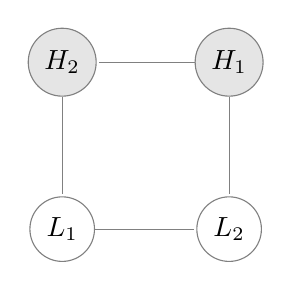
\begin{tikzpicture}[shorten >=1pt,draw=black!50]
	\node (H1) at ( 1.06,  1.06)	[circle, draw, fill = gray!20]	{$H_{1}$};
	\node (H2) at (-1.06,  1.06)	[circle, draw, fill = gray!20]	{$H_{2}$};
	\node (L1) at (-1.06, -1.06)	[circle, draw, fill = white]	{$L_{1}$};
	\node (L2) at ( 1.06, -1.06)	[circle, draw, fill = white]	{$L_{2}$};
	\draw (H1) -- (H2);
	\draw (H1) -- (L2);
	\draw (H2) -- (L1);
	\draw (L1) -- (L2);
\end{tikzpicture}
\end{center}
\columnbreak

\scaleeq{
Equations: \begin{cases}
	e^{H}_{1} \left(\frac{25 \phi}{2} - 2\right) = \alpha + 2 e^{H}_{2} - 3 e^{L}_{1} \theta + 2 e^{L}_{2} \theta - \gamma\\
	e^{H}_{2} \left(\frac{25 \phi}{2} - 2\right) = \alpha + 2 e^{H}_{1} + 2 e^{L}_{1} \theta - 3 e^{L}_{2} \theta - \gamma\\
	e^{L}_{1} \left(\frac{25 \phi}{2 \theta} - 2 \theta\right) = \alpha - 3 e^{H}_{1} + 2 e^{H}_{2} + 2 e^{L}_{2} \theta - \gamma\\
	e^{L}_{2} \left(\frac{25 \phi}{2 \theta} - 2 \theta\right) = \alpha + 2 e^{H}_{1} - 3 e^{H}_{2} + 2 e^{L}_{1} \theta - \gamma
\end{cases}
}\end{multicols}


Optimal efforts:

\scaleeq{
\begin{cases}
	e^{H}_{1} &= \frac{2 \left(\alpha - \gamma\right) \left(5 \phi - 2 \theta^{2}\right)}{125 \phi^{2} - 40 \phi \theta^{2} - 40 \phi + 12 \theta^{2}}\\
	e^{H}_{2} &= \frac{2 \left(\alpha - \gamma\right) \left(5 \phi - 2 \theta^{2}\right)}{125 \phi^{2} - 40 \phi \theta^{2} - 40 \phi + 12 \theta^{2}}\\
	e^{L}_{1} &= \frac{2 \theta \left(\alpha - \gamma\right) \left(5 \phi - 2\right)}{125 \phi^{2} - 40 \phi \theta^{2} - 40 \phi + 12 \theta^{2}}\\
	e^{L}_{2} &= \frac{2 \theta \left(\alpha - \gamma\right) \left(5 \phi - 2\right)}{125 \phi^{2} - 40 \phi \theta^{2} - 40 \phi + 12 \theta^{2}}
\end{cases}
}

Production Costs:

\scaleeq{
\begin{cases}
	c^{H}_{1} &= - \frac{10 \alpha \phi \theta^{2} + 20 \alpha \phi - 12 \alpha \theta^{2} - 125 \gamma \phi^{2} + 30 \gamma \phi \theta^{2} + 20 \gamma \phi}{125 \phi^{2} - 40 \phi \theta^{2} - 40 \phi + 12 \theta^{2}}\\
	c^{H}_{2} &= - \frac{10 \alpha \phi \theta^{2} + 20 \alpha \phi - 12 \alpha \theta^{2} - 125 \gamma \phi^{2} + 30 \gamma \phi \theta^{2} + 20 \gamma \phi}{125 \phi^{2} - 40 \phi \theta^{2} - 40 \phi + 12 \theta^{2}}\\
	c^{L}_{1} &= - \frac{20 \alpha \phi \theta^{2} + 10 \alpha \phi - 12 \alpha \theta^{2} - 125 \gamma \phi^{2} + 20 \gamma \phi \theta^{2} + 30 \gamma \phi}{125 \phi^{2} - 40 \phi \theta^{2} - 40 \phi + 12 \theta^{2}}\\
	c^{L}_{2} &= - \frac{20 \alpha \phi \theta^{2} + 10 \alpha \phi - 12 \alpha \theta^{2} - 125 \gamma \phi^{2} + 20 \gamma \phi \theta^{2} + 30 \gamma \phi}{125 \phi^{2} - 40 \phi \theta^{2} - 40 \phi + 12 \theta^{2}}
\end{cases}
}

Production Quantities:

\scaleeq{
\begin{cases}
	q^{H}_{1} &= \frac{5 \phi \left(\alpha - \gamma\right) \left(5 \phi - 2 \theta^{2}\right)}{125 \phi^{2} - 40 \phi \theta^{2} - 40 \phi + 12 \theta^{2}}\\
	q^{H}_{2} &= \frac{5 \phi \left(\alpha - \gamma\right) \left(5 \phi - 2 \theta^{2}\right)}{125 \phi^{2} - 40 \phi \theta^{2} - 40 \phi + 12 \theta^{2}}\\
	q^{L}_{1} &= \frac{5 \phi \left(\alpha - \gamma\right) \left(5 \phi - 2\right)}{125 \phi^{2} - 40 \phi \theta^{2} - 40 \phi + 12 \theta^{2}}\\
	q^{L}_{2} &= \frac{5 \phi \left(\alpha - \gamma\right) \left(5 \phi - 2\right)}{125 \phi^{2} - 40 \phi \theta^{2} - 40 \phi + 12 \theta^{2}}
\end{cases}
}

Profits:

\begin{equation}
\label{eq:E4E:2H2L_profit}
\scaledequation{\begin{cases}
	\pi^{H}_{1} &= \frac{\phi \left(\alpha - \gamma\right)^{2} \left(5 \phi - 2 \theta^{2}\right)^{2} \left(25 \phi - 4\right)}{\left(125 \phi^{2} - 40 \phi \theta^{2} - 40 \phi + 12 \theta^{2}\right)^{2}}\\
	\pi^{H}_{2} &= \frac{\phi \left(\alpha - \gamma\right)^{2} \left(5 \phi - 2 \theta^{2}\right)^{2} \left(25 \phi - 4\right)}{\left(125 \phi^{2} - 40 \phi \theta^{2} - 40 \phi + 12 \theta^{2}\right)^{2}}\\
	\pi^{L}_{1} &= \frac{\phi \left(\alpha - \gamma\right)^{2} \left(5 \phi - 2\right)^{2} \left(25 \phi - 4 \theta^{2}\right)}{\left(125 \phi^{2} - 40 \phi \theta^{2} - 40 \phi + 12 \theta^{2}\right)^{2}}\\
	\pi^{L}_{2} &= \frac{\phi \left(\alpha - \gamma\right)^{2} \left(5 \phi - 2\right)^{2} \left(25 \phi - 4 \theta^{2}\right)}{\left(125 \phi^{2} - 40 \phi \theta^{2} - 40 \phi + 12 \theta^{2}\right)^{2}}
\end{cases}
}
\end{equation}

Total Production:

\scaleeq{
\frac{20 \phi \left(\alpha - \gamma\right) \left(5 \phi - \theta^{2} - 1\right)}{125 \phi^{2} - 40 \phi \theta^{2} - 40 \phi + 12 \theta^{2}}
}

Price:

\scaleeq{
\frac{25 \alpha \phi^{2} - 20 \alpha \phi \theta^{2} - 20 \alpha \phi + 12 \alpha \theta^{2} + 100 \gamma \phi^{2} - 20 \gamma \phi \theta^{2} - 20 \gamma \phi}{125 \phi^{2} - 40 \phi \theta^{2} - 40 \phi + 12 \theta^{2}}
}

Firm Surplus:

\scaleeq{
\frac{4 \phi \left(\alpha - \gamma\right)^{2} \left(625 \phi^{3} - 300 \phi^{2} \theta^{2} - 300 \phi^{2} + 50 \phi \theta^{4} + 80 \phi \theta^{2} + 50 \phi - 8 \theta^{4} - 8 \theta^{2}\right)}{\left(125 \phi^{2} - 40 \phi \theta^{2} - 40 \phi + 12 \theta^{2}\right)^{2}}
}

Consumer Surplus:

\scaleeq{
\frac{200 \phi^{2} \left(\alpha - \gamma\right)^{2} \left(5 \phi - \theta^{2} - 1\right)^{2}}{\left(125 \phi^{2} - 40 \phi \theta^{2} - 40 \phi + 12 \theta^{2}\right)^{2}}
}

Social Welfare:

\scaleeq{
\frac{4 \phi \left(\alpha - \gamma\right)^{2} \left(1875 \phi^{3} - 800 \phi^{2} \theta^{2} - 800 \phi^{2} + 100 \phi \theta^{4} + 180 \phi \theta^{2} + 100 \phi - 8 \theta^{4} - 8 \theta^{2}\right)}{\left(125 \phi^{2} - 40 \phi \theta^{2} - 40 \phi + 12 \theta^{2}\right)^{2}}
}

%======================================================================

\subsubsection{E4F [2H2L]}
\label{apx:E4F:2H2L}

\begin{multicols}{2}
\begin{center}
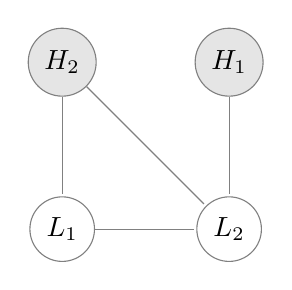
\begin{tikzpicture}[shorten >=1pt,draw=black!50]
	\node (H1) at ( 1.06,  1.06)	[circle, draw, fill = gray!20]	{$H_{1}$};
	\node (H2) at (-1.06,  1.06)	[circle, draw, fill = gray!20]	{$H_{2}$};
	\node (L1) at (-1.06, -1.06)	[circle, draw, fill = white]	{$L_{1}$};
	\node (L2) at ( 1.06, -1.06)	[circle, draw, fill = white]	{$L_{2}$};
	\draw (H1) -- (L2);
	\draw (H2) -- (L1);
	\draw (H2) -- (L2);
	\draw (L1) -- (L2);
\end{tikzpicture}
\end{center}
\columnbreak

\scaleeq{
Equations: \begin{cases}
	e^{H}_{1} \left(\frac{25 \phi}{3} - 3\right) = \alpha - 3 e^{H}_{2} - 3 e^{L}_{1} \theta + e^{L}_{2} \theta - \gamma\\
	e^{H}_{2} \left(\frac{25 \phi}{2} - 2\right) = \alpha - 2 e^{H}_{1} + 2 e^{L}_{1} \theta + e^{L}_{2} \theta - \gamma\\
	e^{L}_{1} \left(\frac{25 \phi}{2 \theta} - 2 \theta\right) = \alpha - 2 e^{H}_{1} + 2 e^{H}_{2} + e^{L}_{2} \theta - \gamma\\
	e^{L}_{2} \left(\frac{25 \phi}{\theta} - \theta\right) = \alpha + 3 e^{H}_{1} + 2 e^{H}_{2} + 2 e^{L}_{1} \theta - \gamma
\end{cases}
}\end{multicols}


Optimal efforts:

\scaleeq{
\begin{cases}
	e^{H}_{1} &= \frac{15 \phi \left(\alpha - \gamma\right) \left(5 \phi - 2 \theta^{2} - 2\right)}{625 \phi^{3} - 125 \phi^{2} \theta^{2} - 325 \phi^{2} + 6 \theta^{4} + 6 \theta^{2}}\\
	e^{H}_{2} &= \frac{10 \phi \left(\alpha - \gamma\right) \left(5 \phi - 3\right)}{625 \phi^{3} - 125 \phi^{2} \theta^{2} - 325 \phi^{2} + 6 \theta^{4} + 6 \theta^{2}}\\
	e^{L}_{1} &= \frac{10 \phi \theta \left(\alpha - \gamma\right) \left(5 \phi - 3\right)}{625 \phi^{3} - 125 \phi^{2} \theta^{2} - 325 \phi^{2} + 6 \theta^{4} + 6 \theta^{2}}\\
	e^{L}_{2} &= \frac{\theta \left(\alpha - \gamma\right) \left(25 \phi^{2} - 6 \theta^{2} - 6\right)}{625 \phi^{3} - 125 \phi^{2} \theta^{2} - 325 \phi^{2} + 6 \theta^{4} + 6 \theta^{2}}
\end{cases}
}

Production Costs:

\scaleeq{
\begin{cases}
	c^{H}_{1} &= - \frac{25 \alpha \phi^{2} \theta^{2} + 75 \alpha \phi^{2} - 30 \alpha \phi \theta^{2} - 30 \alpha \phi - 6 \alpha \theta^{4} - 6 \alpha \theta^{2} - 625 \gamma \phi^{3} + 100 \gamma \phi^{2} \theta^{2} + 250 \gamma \phi^{2} + 30 \gamma \phi \theta^{2} + 30 \gamma \phi}{625 \phi^{3} - 125 \phi^{2} \theta^{2} - 325 \phi^{2} + 6 \theta^{4} + 6 \theta^{2}}\\
	c^{H}_{2} &= - \frac{75 \alpha \phi^{2} \theta^{2} + 50 \alpha \phi^{2} - 30 \alpha \phi \theta^{2} - 30 \alpha \phi - 6 \alpha \theta^{4} - 6 \alpha \theta^{2} - 625 \gamma \phi^{3} + 50 \gamma \phi^{2} \theta^{2} + 275 \gamma \phi^{2} + 30 \gamma \phi \theta^{2} + 30 \gamma \phi}{625 \phi^{3} - 125 \phi^{2} \theta^{2} - 325 \phi^{2} + 6 \theta^{4} + 6 \theta^{2}}\\
	c^{L}_{1} &= - \frac{75 \alpha \phi^{2} \theta^{2} + 50 \alpha \phi^{2} - 30 \alpha \phi \theta^{2} - 30 \alpha \phi - 6 \alpha \theta^{4} - 6 \alpha \theta^{2} - 625 \gamma \phi^{3} + 50 \gamma \phi^{2} \theta^{2} + 275 \gamma \phi^{2} + 30 \gamma \phi \theta^{2} + 30 \gamma \phi}{625 \phi^{3} - 125 \phi^{2} \theta^{2} - 325 \phi^{2} + 6 \theta^{4} + 6 \theta^{2}}\\
	c^{L}_{2} &= - \frac{75 \alpha \phi^{2} \theta^{2} + 125 \alpha \phi^{2} - 60 \alpha \phi \theta^{2} - 60 \alpha \phi - 6 \alpha \theta^{4} - 6 \alpha \theta^{2} - 625 \gamma \phi^{3} + 50 \gamma \phi^{2} \theta^{2} + 200 \gamma \phi^{2} + 60 \gamma \phi \theta^{2} + 60 \gamma \phi}{625 \phi^{3} - 125 \phi^{2} \theta^{2} - 325 \phi^{2} + 6 \theta^{4} + 6 \theta^{2}}
\end{cases}
}

Production Quantities:

\scaleeq{
\begin{cases}
	q^{H}_{1} &= \frac{25 \phi^{2} \left(\alpha - \gamma\right) \left(5 \phi - 2 \theta^{2} - 2\right)}{625 \phi^{3} - 125 \phi^{2} \theta^{2} - 325 \phi^{2} + 6 \theta^{4} + 6 \theta^{2}}\\
	q^{H}_{2} &= \frac{25 \phi^{2} \left(\alpha - \gamma\right) \left(5 \phi - 3\right)}{625 \phi^{3} - 125 \phi^{2} \theta^{2} - 325 \phi^{2} + 6 \theta^{4} + 6 \theta^{2}}\\
	q^{L}_{1} &= \frac{25 \phi^{2} \left(\alpha - \gamma\right) \left(5 \phi - 3\right)}{625 \phi^{3} - 125 \phi^{2} \theta^{2} - 325 \phi^{2} + 6 \theta^{4} + 6 \theta^{2}}\\
	q^{L}_{2} &= \frac{5 \phi \left(\alpha - \gamma\right) \left(25 \phi^{2} - 6 \theta^{2} - 6\right)}{625 \phi^{3} - 125 \phi^{2} \theta^{2} - 325 \phi^{2} + 6 \theta^{4} + 6 \theta^{2}}
\end{cases}
}

Profits:

\begin{equation}
\label{eq:E4F:2H2L_profit}
\scaledequation{\begin{cases}
	\pi^{H}_{1} &= \frac{25 \phi^{3} \left(\alpha - \gamma\right)^{2} \left(25 \phi - 9\right) \left(5 \phi - 2 \theta^{2} - 2\right)^{2}}{\left(625 \phi^{3} - 125 \phi^{2} \theta^{2} - 325 \phi^{2} + 6 \theta^{4} + 6 \theta^{2}\right)^{2}}\\
	\pi^{H}_{2} &= \frac{25 \phi^{3} \left(\alpha - \gamma\right)^{2} \left(5 \phi - 3\right)^{2} \left(25 \phi - 4\right)}{\left(625 \phi^{3} - 125 \phi^{2} \theta^{2} - 325 \phi^{2} + 6 \theta^{4} + 6 \theta^{2}\right)^{2}}\\
	\pi^{L}_{1} &= \frac{25 \phi^{3} \left(\alpha - \gamma\right)^{2} \left(5 \phi - 3\right)^{2} \left(25 \phi - 4 \theta^{2}\right)}{\left(625 \phi^{3} - 125 \phi^{2} \theta^{2} - 325 \phi^{2} + 6 \theta^{4} + 6 \theta^{2}\right)^{2}}\\
	\pi^{L}_{2} &= \frac{\phi \left(\alpha - \gamma\right)^{2} \left(25 \phi - \theta^{2}\right) \left(25 \phi^{2} - 6 \theta^{2} - 6\right)^{2}}{\left(625 \phi^{3} - 125 \phi^{2} \theta^{2} - 325 \phi^{2} + 6 \theta^{4} + 6 \theta^{2}\right)^{2}}
\end{cases}
}
\end{equation}

Total Production:

\scaleeq{
\frac{10 \phi \left(\alpha - \gamma\right) \left(50 \phi^{2} - 5 \phi \theta^{2} - 20 \phi - 3 \theta^{2} - 3\right)}{625 \phi^{3} - 125 \phi^{2} \theta^{2} - 325 \phi^{2} + 6 \theta^{4} + 6 \theta^{2}}
}

Price:

\scaleeq{
\frac{125 \alpha \phi^{3} - 75 \alpha \phi^{2} \theta^{2} - 125 \alpha \phi^{2} + 30 \alpha \phi \theta^{2} + 30 \alpha \phi + 6 \alpha \theta^{4} + 6 \alpha \theta^{2} + 500 \gamma \phi^{3} - 50 \gamma \phi^{2} \theta^{2} - 200 \gamma \phi^{2} - 30 \gamma \phi \theta^{2} - 30 \gamma \phi}{625 \phi^{3} - 125 \phi^{2} \theta^{2} - 325 \phi^{2} + 6 \theta^{4} + 6 \theta^{2}}
}

Firm Surplus:

\scaleeq{
\frac{\phi \left(\alpha - \gamma\right)^{2} \left(62500 \phi^{5} - 15625 \phi^{4} \theta^{2} - 58125 \phi^{4} + 2500 \phi^{3} \theta^{4} + 5000 \phi^{3} \theta^{2} + 13750 \phi^{3} - 600 \phi^{2} \theta^{4} - 2400 \phi^{2} \theta^{2} - 1800 \phi^{2} + 900 \phi \theta^{4} + 1800 \phi \theta^{2} + 900 \phi - 36 \theta^{6} - 72 \theta^{4} - 36 \theta^{2}\right)}{\left(625 \phi^{3} - 125 \phi^{2} \theta^{2} - 325 \phi^{2} + 6 \theta^{4} + 6 \theta^{2}\right)^{2}}
}

Consumer Surplus:

\scaleeq{
\frac{50 \phi^{2} \left(\alpha - \gamma\right)^{2} \left(50 \phi^{2} - 5 \phi \theta^{2} - 20 \phi - 3 \theta^{2} - 3\right)^{2}}{\left(625 \phi^{3} - 125 \phi^{2} \theta^{2} - 325 \phi^{2} + 6 \theta^{4} + 6 \theta^{2}\right)^{2}}
}

Social Welfare:

\scaleeq{
\frac{\phi \left(\alpha - \gamma\right)^{2} \left(187500 \phi^{5} - 40625 \phi^{4} \theta^{2} - 158125 \phi^{4} + 3750 \phi^{3} \theta^{4} + 18750 \phi^{3} + 900 \phi^{2} \theta^{4} + 5100 \phi^{2} \theta^{2} + 4200 \phi^{2} + 1350 \phi \theta^{4} + 2700 \phi \theta^{2} + 1350 \phi - 36 \theta^{6} - 72 \theta^{4} - 36 \theta^{2}\right)}{\left(625 \phi^{3} - 125 \phi^{2} \theta^{2} - 325 \phi^{2} + 6 \theta^{4} + 6 \theta^{2}\right)^{2}}
}

%======================================================================

\subsubsection{E5A [2H2L]}
\label{apx:E5A:2H2L}

\begin{multicols}{2}
\begin{center}
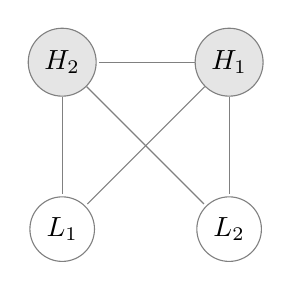
\begin{tikzpicture}[shorten >=1pt,draw=black!50]
	\node (H1) at ( 1.06,  1.06)	[circle, draw, fill = gray!20]	{$H_{1}$};
	\node (H2) at (-1.06,  1.06)	[circle, draw, fill = gray!20]	{$H_{2}$};
	\node (L1) at (-1.06, -1.06)	[circle, draw, fill = white]	{$L_{1}$};
	\node (L2) at ( 1.06, -1.06)	[circle, draw, fill = white]	{$L_{2}$};
	\draw (H1) -- (H2);
	\draw (H1) -- (L1);
	\draw (H1) -- (L2);
	\draw (H2) -- (L1);
	\draw (H2) -- (L2);
\end{tikzpicture}
\end{center}
\columnbreak

\scaleeq{
Equations: \begin{cases}
	e^{H}_{1} \left(25 \phi - 1\right) = \alpha + e^{H}_{2} + 2 e^{L}_{1} \theta + 2 e^{L}_{2} \theta - \gamma\\
	e^{H}_{2} \left(25 \phi - 1\right) = \alpha + e^{H}_{1} + 2 e^{L}_{1} \theta + 2 e^{L}_{2} \theta - \gamma\\
	e^{L}_{1} \left(\frac{25 \phi}{2 \theta} - 2 \theta\right) = \alpha + e^{H}_{1} + e^{H}_{2} - 3 e^{L}_{2} \theta - \gamma\\
	e^{L}_{2} \left(\frac{25 \phi}{2 \theta} - 2 \theta\right) = \alpha + e^{H}_{1} + e^{H}_{2} - 3 e^{L}_{1} \theta - \gamma
\end{cases}
}\end{multicols}


Optimal efforts:

\scaleeq{
\begin{cases}
	e^{H}_{1} &= \frac{\left(\alpha - \gamma\right) \left(5 \phi + 2 \theta^{2}\right)}{125 \phi^{2} + 10 \phi \theta^{2} - 10 \phi - 4 \theta^{2}}\\
	e^{H}_{2} &= \frac{\left(\alpha - \gamma\right) \left(5 \phi + 2 \theta^{2}\right)}{125 \phi^{2} + 10 \phi \theta^{2} - 10 \phi - 4 \theta^{2}}\\
	e^{L}_{1} &= \frac{10 \phi \theta \left(\alpha - \gamma\right)}{125 \phi^{2} + 10 \phi \theta^{2} - 10 \phi - 4 \theta^{2}}\\
	e^{L}_{2} &= \frac{10 \phi \theta \left(\alpha - \gamma\right)}{125 \phi^{2} + 10 \phi \theta^{2} - 10 \phi - 4 \theta^{2}}
\end{cases}
}

Production Costs:

\scaleeq{
\begin{cases}
	c^{H}_{1} &= - \frac{20 \alpha \phi \theta^{2} + 10 \alpha \phi + 4 \alpha \theta^{2} - 125 \gamma \phi^{2} - 30 \gamma \phi \theta^{2}}{125 \phi^{2} + 10 \phi \theta^{2} - 10 \phi - 4 \theta^{2}}\\
	c^{H}_{2} &= - \frac{20 \alpha \phi \theta^{2} + 10 \alpha \phi + 4 \alpha \theta^{2} - 125 \gamma \phi^{2} - 30 \gamma \phi \theta^{2}}{125 \phi^{2} + 10 \phi \theta^{2} - 10 \phi - 4 \theta^{2}}\\
	c^{L}_{1} &= - \frac{10 \alpha \phi \theta^{2} + 10 \alpha \phi + 4 \alpha \theta^{2} - 125 \gamma \phi^{2} - 20 \gamma \phi \theta^{2}}{125 \phi^{2} + 10 \phi \theta^{2} - 10 \phi - 4 \theta^{2}}\\
	c^{L}_{2} &= - \frac{10 \alpha \phi \theta^{2} + 10 \alpha \phi + 4 \alpha \theta^{2} - 125 \gamma \phi^{2} - 20 \gamma \phi \theta^{2}}{125 \phi^{2} + 10 \phi \theta^{2} - 10 \phi - 4 \theta^{2}}
\end{cases}
}

Production Quantities:

\scaleeq{
\begin{cases}
	q^{H}_{1} &= \frac{5 \phi \left(\alpha - \gamma\right) \left(5 \phi + 2 \theta^{2}\right)}{125 \phi^{2} + 10 \phi \theta^{2} - 10 \phi - 4 \theta^{2}}\\
	q^{H}_{2} &= \frac{5 \phi \left(\alpha - \gamma\right) \left(5 \phi + 2 \theta^{2}\right)}{125 \phi^{2} + 10 \phi \theta^{2} - 10 \phi - 4 \theta^{2}}\\
	q^{L}_{1} &= \frac{25 \phi^{2} \left(\alpha - \gamma\right)}{125 \phi^{2} + 10 \phi \theta^{2} - 10 \phi - 4 \theta^{2}}\\
	q^{L}_{2} &= \frac{25 \phi^{2} \left(\alpha - \gamma\right)}{125 \phi^{2} + 10 \phi \theta^{2} - 10 \phi - 4 \theta^{2}}
\end{cases}
}

Profits:

\begin{equation}
\label{eq:E5A:2H2L_profit}
\scaledequation{\begin{cases}
	\pi^{H}_{1} &= \frac{\phi \left(\alpha - \gamma\right)^{2} \left(5 \phi + 2 \theta^{2}\right)^{2} \left(25 \phi - 1\right)}{\left(125 \phi^{2} + 10 \phi \theta^{2} - 10 \phi - 4 \theta^{2}\right)^{2}}\\
	\pi^{H}_{2} &= \frac{\phi \left(\alpha - \gamma\right)^{2} \left(5 \phi + 2 \theta^{2}\right)^{2} \left(25 \phi - 1\right)}{\left(125 \phi^{2} + 10 \phi \theta^{2} - 10 \phi - 4 \theta^{2}\right)^{2}}\\
	\pi^{L}_{1} &= \frac{25 \phi^{3} \left(\alpha - \gamma\right)^{2} \left(25 \phi - 4 \theta^{2}\right)}{\left(125 \phi^{2} + 10 \phi \theta^{2} - 10 \phi - 4 \theta^{2}\right)^{2}}\\
	\pi^{L}_{2} &= \frac{25 \phi^{3} \left(\alpha - \gamma\right)^{2} \left(25 \phi - 4 \theta^{2}\right)}{\left(125 \phi^{2} + 10 \phi \theta^{2} - 10 \phi - 4 \theta^{2}\right)^{2}}
\end{cases}
}
\end{equation}

Total Production:

\scaleeq{
\frac{20 \phi \left(\alpha - \gamma\right) \left(5 \phi + \theta^{2}\right)}{125 \phi^{2} + 10 \phi \theta^{2} - 10 \phi - 4 \theta^{2}}
}

Price:

\scaleeq{
\frac{25 \alpha \phi^{2} - 10 \alpha \phi \theta^{2} - 10 \alpha \phi - 4 \alpha \theta^{2} + 100 \gamma \phi^{2} + 20 \gamma \phi \theta^{2}}{125 \phi^{2} + 10 \phi \theta^{2} - 10 \phi - 4 \theta^{2}}
}

Firm Surplus:

\scaleeq{
\frac{2 \phi \left(\alpha - \gamma\right)^{2} \left(1250 \phi^{3} + 400 \phi^{2} \theta^{2} - 25 \phi^{2} + 100 \phi \theta^{4} - 20 \phi \theta^{2} - 4 \theta^{4}\right)}{\left(125 \phi^{2} + 10 \phi \theta^{2} - 10 \phi - 4 \theta^{2}\right)^{2}}
}

Consumer Surplus:

\scaleeq{
\frac{200 \phi^{2} \left(\alpha - \gamma\right)^{2} \left(5 \phi + \theta^{2}\right)^{2}}{\left(125 \phi^{2} + 10 \phi \theta^{2} - 10 \phi - 4 \theta^{2}\right)^{2}}
}

Social Welfare:

\scaleeq{
\frac{2 \phi \left(\alpha - \gamma\right)^{2} \left(3750 \phi^{3} + 1400 \phi^{2} \theta^{2} - 25 \phi^{2} + 200 \phi \theta^{4} - 20 \phi \theta^{2} - 4 \theta^{4}\right)}{\left(125 \phi^{2} + 10 \phi \theta^{2} - 10 \phi - 4 \theta^{2}\right)^{2}}
}

%======================================================================

\subsubsection{E5B [2H2L]}
\label{apx:E5B:2H2L}

\begin{multicols}{2}
\begin{center}
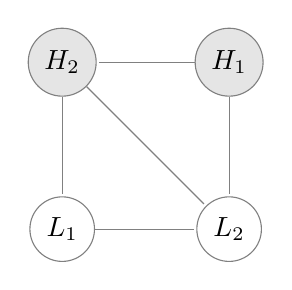
\begin{tikzpicture}[shorten >=1pt,draw=black!50]
	\node (H1) at ( 1.06,  1.06)	[circle, draw, fill = gray!20]	{$H_{1}$};
	\node (H2) at (-1.06,  1.06)	[circle, draw, fill = gray!20]	{$H_{2}$};
	\node (L1) at (-1.06, -1.06)	[circle, draw, fill = white]	{$L_{1}$};
	\node (L2) at ( 1.06, -1.06)	[circle, draw, fill = white]	{$L_{2}$};
	\draw (H1) -- (H2);
	\draw (H1) -- (L2);
	\draw (H2) -- (L1);
	\draw (H2) -- (L2);
	\draw (L1) -- (L2);
\end{tikzpicture}
\end{center}
\columnbreak

\scaleeq{
Equations: \begin{cases}
	e^{H}_{1} \left(\frac{25 \phi}{2} - 2\right) = \alpha + e^{H}_{2} - 3 e^{L}_{1} \theta + e^{L}_{2} \theta - \gamma\\
	e^{H}_{2} \left(25 \phi - 1\right) = \alpha + 2 e^{H}_{1} + 2 e^{L}_{1} \theta + e^{L}_{2} \theta - \gamma\\
	e^{L}_{1} \left(\frac{25 \phi}{2 \theta} - 2 \theta\right) = \alpha - 3 e^{H}_{1} + e^{H}_{2} + e^{L}_{2} \theta - \gamma\\
	e^{L}_{2} \left(\frac{25 \phi}{\theta} - \theta\right) = \alpha + 2 e^{H}_{1} + e^{H}_{2} + 2 e^{L}_{1} \theta - \gamma
\end{cases}
}\end{multicols}


Optimal efforts:

\scaleeq{
\begin{cases}
	e^{H}_{1} &= \frac{10 \phi \left(\alpha - \gamma\right) \left(5 \phi - 2 \theta^{2}\right)}{\left(125 \phi^{2} - 4 \theta^{2}\right) \left(5 \phi - \theta^{2} - 1\right)}\\
	e^{H}_{2} &= \frac{\left(\alpha - \gamma\right) \left(5 \phi - 2 \theta\right) \left(5 \phi + 2 \theta\right)}{\left(125 \phi^{2} - 4 \theta^{2}\right) \left(5 \phi - \theta^{2} - 1\right)}\\
	e^{L}_{1} &= \frac{10 \phi \theta \left(\alpha - \gamma\right) \left(5 \phi - 2\right)}{\left(125 \phi^{2} - 4 \theta^{2}\right) \left(5 \phi - \theta^{2} - 1\right)}\\
	e^{L}_{2} &= \frac{\theta \left(\alpha - \gamma\right) \left(5 \phi - 2 \theta\right) \left(5 \phi + 2 \theta\right)}{\left(125 \phi^{2} - 4 \theta^{2}\right) \left(5 \phi - \theta^{2} - 1\right)}
\end{cases}
}

Production Costs:

\scaleeq{
\begin{cases}
	c^{H}_{1} &= - \frac{25 \alpha \phi^{2} \theta^{2} + 75 \alpha \phi^{2} - 20 \alpha \phi \theta^{2} - 4 \alpha \theta^{4} - 4 \alpha \theta^{2} - 625 \gamma \phi^{3} + 100 \gamma \phi^{2} \theta^{2} + 50 \gamma \phi^{2} + 40 \gamma \phi \theta^{2}}{\left(125 \phi^{2} - 4 \theta^{2}\right) \left(5 \phi - \theta^{2} - 1\right)}\\
	c^{H}_{2} &= - \frac{75 \alpha \phi^{2} \theta^{2} + 75 \alpha \phi^{2} - 40 \alpha \phi \theta^{2} - 4 \alpha \theta^{4} - 4 \alpha \theta^{2} - 625 \gamma \phi^{3} + 50 \gamma \phi^{2} \theta^{2} + 50 \gamma \phi^{2} + 60 \gamma \phi \theta^{2}}{\left(125 \phi^{2} - 4 \theta^{2}\right) \left(5 \phi - \theta^{2} - 1\right)}\\
	c^{L}_{1} &= - \frac{75 \alpha \phi^{2} \theta^{2} + 25 \alpha \phi^{2} - 20 \alpha \phi \theta^{2} - 4 \alpha \theta^{4} - 4 \alpha \theta^{2} - 625 \gamma \phi^{3} + 50 \gamma \phi^{2} \theta^{2} + 100 \gamma \phi^{2} + 40 \gamma \phi \theta^{2}}{\left(125 \phi^{2} - 4 \theta^{2}\right) \left(5 \phi - \theta^{2} - 1\right)}\\
	c^{L}_{2} &= - \frac{75 \alpha \phi^{2} \theta^{2} + 75 \alpha \phi^{2} - 40 \alpha \phi \theta^{2} - 4 \alpha \theta^{4} - 4 \alpha \theta^{2} - 625 \gamma \phi^{3} + 50 \gamma \phi^{2} \theta^{2} + 50 \gamma \phi^{2} + 60 \gamma \phi \theta^{2}}{\left(125 \phi^{2} - 4 \theta^{2}\right) \left(5 \phi - \theta^{2} - 1\right)}
\end{cases}
}

Production Quantities:

\scaleeq{
\begin{cases}
	q^{H}_{1} &= \frac{25 \phi^{2} \left(\alpha - \gamma\right) \left(5 \phi - 2 \theta^{2}\right)}{\left(125 \phi^{2} - 4 \theta^{2}\right) \left(5 \phi - \theta^{2} - 1\right)}\\
	q^{H}_{2} &= \frac{5 \phi \left(\alpha - \gamma\right) \left(5 \phi - 2 \theta\right) \left(5 \phi + 2 \theta\right)}{\left(125 \phi^{2} - 4 \theta^{2}\right) \left(5 \phi - \theta^{2} - 1\right)}\\
	q^{L}_{1} &= \frac{25 \phi^{2} \left(\alpha - \gamma\right) \left(5 \phi - 2\right)}{\left(125 \phi^{2} - 4 \theta^{2}\right) \left(5 \phi - \theta^{2} - 1\right)}\\
	q^{L}_{2} &= \frac{5 \phi \left(\alpha - \gamma\right) \left(5 \phi - 2 \theta\right) \left(5 \phi + 2 \theta\right)}{\left(125 \phi^{2} - 4 \theta^{2}\right) \left(5 \phi - \theta^{2} - 1\right)}
\end{cases}
}

Profits:

\begin{equation}
\label{eq:E5B:2H2L_profit}
\scaledequation{\begin{cases}
	\pi^{H}_{1} &= \frac{25 \phi^{3} \left(\alpha - \gamma\right)^{2} \left(5 \phi - 2 \theta^{2}\right)^{2} \left(25 \phi - 4\right)}{\left(125 \phi^{2} - 4 \theta^{2}\right)^{2} \left(5 \phi - \theta^{2} - 1\right)^{2}}\\
	\pi^{H}_{2} &= \frac{\phi \left(\alpha - \gamma\right)^{2} \left(5 \phi - 2 \theta\right)^{2} \left(5 \phi + 2 \theta\right)^{2} \left(25 \phi - 1\right)}{\left(125 \phi^{2} - 4 \theta^{2}\right)^{2} \left(5 \phi - \theta^{2} - 1\right)^{2}}\\
	\pi^{L}_{1} &= \frac{25 \phi^{3} \left(\alpha - \gamma\right)^{2} \left(5 \phi - 2\right)^{2} \left(25 \phi - 4 \theta^{2}\right)}{\left(125 \phi^{2} - 4 \theta^{2}\right)^{2} \left(5 \phi - \theta^{2} - 1\right)^{2}}\\
	\pi^{L}_{2} &= \frac{\phi \left(\alpha - \gamma\right)^{2} \left(5 \phi - 2 \theta\right)^{2} \left(5 \phi + 2 \theta\right)^{2} \left(25 \phi - \theta^{2}\right)}{\left(125 \phi^{2} - 4 \theta^{2}\right)^{2} \left(5 \phi - \theta^{2} - 1\right)^{2}}
\end{cases}
}
\end{equation}

Total Production:

\scaleeq{
\frac{10 \phi \left(\alpha - \gamma\right) \left(50 \phi^{2} - 5 \phi \theta^{2} - 5 \phi - 4 \theta^{2}\right)}{\left(125 \phi^{2} - 4 \theta^{2}\right) \left(5 \phi - \theta^{2} - 1\right)}
}

Price:

\scaleeq{
\frac{125 \alpha \phi^{3} - 75 \alpha \phi^{2} \theta^{2} - 75 \alpha \phi^{2} + 20 \alpha \phi \theta^{2} + 4 \alpha \theta^{4} + 4 \alpha \theta^{2} + 500 \gamma \phi^{3} - 50 \gamma \phi^{2} \theta^{2} - 50 \gamma \phi^{2} - 40 \gamma \phi \theta^{2}}{\left(125 \phi^{2} - 4 \theta^{2}\right) \left(5 \phi - \theta^{2} - 1\right)}
}

Firm Surplus:

\scaleeq{
\frac{\phi \left(\alpha - \gamma\right)^{2} \left(62500 \phi^{5} - 15625 \phi^{4} \theta^{2} - 15625 \phi^{4} + 2500 \phi^{3} \theta^{4} - 6000 \phi^{3} \theta^{2} + 2500 \phi^{3} - 200 \phi^{2} \theta^{4} - 200 \phi^{2} \theta^{2} + 800 \phi \theta^{4} - 16 \theta^{6} - 16 \theta^{4}\right)}{\left(125 \phi^{2} - 4 \theta^{2}\right)^{2} \left(5 \phi - \theta^{2} - 1\right)^{2}}
}

Consumer Surplus:

\scaleeq{
\frac{50 \phi^{2} \left(\alpha - \gamma\right)^{2} \left(50 \phi^{2} - 5 \phi \theta^{2} - 5 \phi - 4 \theta^{2}\right)^{2}}{\left(125 \phi^{2} - 4 \theta^{2}\right)^{2} \left(5 \phi - \theta^{2} - 1\right)^{2}}
}

Social Welfare:

\scaleeq{
\frac{\phi \left(\alpha - \gamma\right)^{2} \left(187500 \phi^{5} - 40625 \phi^{4} \theta^{2} - 40625 \phi^{4} + 3750 \phi^{3} \theta^{4} - 23500 \phi^{3} \theta^{2} + 3750 \phi^{3} + 1800 \phi^{2} \theta^{4} + 1800 \phi^{2} \theta^{2} + 1600 \phi \theta^{4} - 16 \theta^{6} - 16 \theta^{4}\right)}{\left(125 \phi^{2} - 4 \theta^{2}\right)^{2} \left(5 \phi - \theta^{2} - 1\right)^{2}}
}

%======================================================================

\subsubsection{E5C [2H2L]}
\label{apx:E5C:2H2L}

\begin{multicols}{2}
\begin{center}
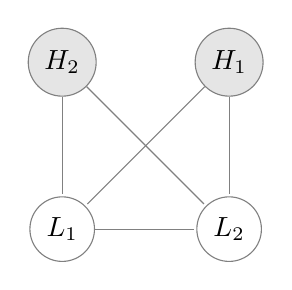
\begin{tikzpicture}[shorten >=1pt,draw=black!50]
	\node (H1) at ( 1.06,  1.06)	[circle, draw, fill = gray!20]	{$H_{1}$};
	\node (H2) at (-1.06,  1.06)	[circle, draw, fill = gray!20]	{$H_{2}$};
	\node (L1) at (-1.06, -1.06)	[circle, draw, fill = white]	{$L_{1}$};
	\node (L2) at ( 1.06, -1.06)	[circle, draw, fill = white]	{$L_{2}$};
	\draw (H1) -- (L1);
	\draw (H1) -- (L2);
	\draw (H2) -- (L1);
	\draw (H2) -- (L2);
	\draw (L1) -- (L2);
\end{tikzpicture}
\end{center}
\columnbreak

\scaleeq{
Equations: \begin{cases}
	e^{H}_{1} \left(\frac{25 \phi}{2} - 2\right) = \alpha - 3 e^{H}_{2} + e^{L}_{1} \theta + e^{L}_{2} \theta - \gamma\\
	e^{H}_{2} \left(\frac{25 \phi}{2} - 2\right) = \alpha - 3 e^{H}_{1} + e^{L}_{1} \theta + e^{L}_{2} \theta - \gamma\\
	e^{L}_{1} \left(\frac{25 \phi}{\theta} - \theta\right) = \alpha + 2 e^{H}_{1} + 2 e^{H}_{2} + e^{L}_{2} \theta - \gamma\\
	e^{L}_{2} \left(\frac{25 \phi}{\theta} - \theta\right) = \alpha + 2 e^{H}_{1} + 2 e^{H}_{2} + e^{L}_{1} \theta - \gamma
\end{cases}
}\end{multicols}


Optimal efforts:

\scaleeq{
\begin{cases}
	e^{H}_{1} &= \frac{10 \phi \left(\alpha - \gamma\right)}{125 \phi^{2} - 10 \phi \theta^{2} + 10 \phi - 4 \theta^{2}}\\
	e^{H}_{2} &= \frac{10 \phi \left(\alpha - \gamma\right)}{125 \phi^{2} - 10 \phi \theta^{2} + 10 \phi - 4 \theta^{2}}\\
	e^{L}_{1} &= \frac{\theta \left(\alpha - \gamma\right) \left(5 \phi + 2\right)}{125 \phi^{2} - 10 \phi \theta^{2} + 10 \phi - 4 \theta^{2}}\\
	e^{L}_{2} &= \frac{\theta \left(\alpha - \gamma\right) \left(5 \phi + 2\right)}{125 \phi^{2} - 10 \phi \theta^{2} + 10 \phi - 4 \theta^{2}}
\end{cases}
}

Production Costs:

\scaleeq{
\begin{cases}
	c^{H}_{1} &= - \frac{10 \alpha \phi \theta^{2} + 10 \alpha \phi + 4 \alpha \theta^{2} - 125 \gamma \phi^{2} - 20 \gamma \phi}{125 \phi^{2} - 10 \phi \theta^{2} + 10 \phi - 4 \theta^{2}}\\
	c^{H}_{2} &= - \frac{10 \alpha \phi \theta^{2} + 10 \alpha \phi + 4 \alpha \theta^{2} - 125 \gamma \phi^{2} - 20 \gamma \phi}{125 \phi^{2} - 10 \phi \theta^{2} + 10 \phi - 4 \theta^{2}}\\
	c^{L}_{1} &= - \frac{10 \alpha \phi \theta^{2} + 20 \alpha \phi + 4 \alpha \theta^{2} - 125 \gamma \phi^{2} - 30 \gamma \phi}{125 \phi^{2} - 10 \phi \theta^{2} + 10 \phi - 4 \theta^{2}}\\
	c^{L}_{2} &= - \frac{10 \alpha \phi \theta^{2} + 20 \alpha \phi + 4 \alpha \theta^{2} - 125 \gamma \phi^{2} - 30 \gamma \phi}{125 \phi^{2} - 10 \phi \theta^{2} + 10 \phi - 4 \theta^{2}}
\end{cases}
}

Production Quantities:

\scaleeq{
\begin{cases}
	q^{H}_{1} &= \frac{25 \phi^{2} \left(\alpha - \gamma\right)}{125 \phi^{2} - 10 \phi \theta^{2} + 10 \phi - 4 \theta^{2}}\\
	q^{H}_{2} &= \frac{25 \phi^{2} \left(\alpha - \gamma\right)}{125 \phi^{2} - 10 \phi \theta^{2} + 10 \phi - 4 \theta^{2}}\\
	q^{L}_{1} &= \frac{5 \phi \left(\alpha - \gamma\right) \left(5 \phi + 2\right)}{125 \phi^{2} - 10 \phi \theta^{2} + 10 \phi - 4 \theta^{2}}\\
	q^{L}_{2} &= \frac{5 \phi \left(\alpha - \gamma\right) \left(5 \phi + 2\right)}{125 \phi^{2} - 10 \phi \theta^{2} + 10 \phi - 4 \theta^{2}}
\end{cases}
}

Profits:

\begin{equation}
\label{eq:E5C:2H2L_profit}
\scaledequation{\begin{cases}
	\pi^{H}_{1} &= \frac{25 \phi^{3} \left(\alpha - \gamma\right)^{2} \left(25 \phi - 4\right)}{\left(125 \phi^{2} - 10 \phi \theta^{2} + 10 \phi - 4 \theta^{2}\right)^{2}}\\
	\pi^{H}_{2} &= \frac{25 \phi^{3} \left(\alpha - \gamma\right)^{2} \left(25 \phi - 4\right)}{\left(125 \phi^{2} - 10 \phi \theta^{2} + 10 \phi - 4 \theta^{2}\right)^{2}}\\
	\pi^{L}_{1} &= \frac{\phi \left(\alpha - \gamma\right)^{2} \left(5 \phi + 2\right)^{2} \left(25 \phi - \theta^{2}\right)}{\left(125 \phi^{2} - 10 \phi \theta^{2} + 10 \phi - 4 \theta^{2}\right)^{2}}\\
	\pi^{L}_{2} &= \frac{\phi \left(\alpha - \gamma\right)^{2} \left(5 \phi + 2\right)^{2} \left(25 \phi - \theta^{2}\right)}{\left(125 \phi^{2} - 10 \phi \theta^{2} + 10 \phi - 4 \theta^{2}\right)^{2}}
\end{cases}
}
\end{equation}

Total Production:

\scaleeq{
\frac{20 \phi \left(\alpha - \gamma\right) \left(5 \phi + 1\right)}{125 \phi^{2} - 10 \phi \theta^{2} + 10 \phi - 4 \theta^{2}}
}

Price:

\scaleeq{
\frac{25 \alpha \phi^{2} - 10 \alpha \phi \theta^{2} - 10 \alpha \phi - 4 \alpha \theta^{2} + 100 \gamma \phi^{2} + 20 \gamma \phi}{125 \phi^{2} - 10 \phi \theta^{2} + 10 \phi - 4 \theta^{2}}
}

Firm Surplus:

\scaleeq{
\frac{2 \phi \left(\alpha - \gamma\right)^{2} \left(1250 \phi^{3} - 25 \phi^{2} \theta^{2} + 400 \phi^{2} - 20 \phi \theta^{2} + 100 \phi - 4 \theta^{2}\right)}{\left(125 \phi^{2} - 10 \phi \theta^{2} + 10 \phi - 4 \theta^{2}\right)^{2}}
}

Consumer Surplus:

\scaleeq{
\frac{200 \phi^{2} \left(\alpha - \gamma\right)^{2} \left(5 \phi + 1\right)^{2}}{\left(125 \phi^{2} - 10 \phi \theta^{2} + 10 \phi - 4 \theta^{2}\right)^{2}}
}

Social Welfare:

\scaleeq{
\frac{2 \phi \left(\alpha - \gamma\right)^{2} \left(3750 \phi^{3} - 25 \phi^{2} \theta^{2} + 1400 \phi^{2} - 20 \phi \theta^{2} + 200 \phi - 4 \theta^{2}\right)}{\left(125 \phi^{2} - 10 \phi \theta^{2} + 10 \phi - 4 \theta^{2}\right)^{2}}
}

%======================================================================

\subsubsection{E6A [2H2L]}
\label{apx:E6A:2H2L}

\begin{multicols}{2}
\begin{center}
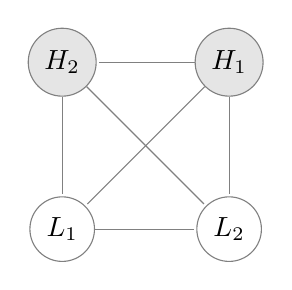
\begin{tikzpicture}[shorten >=1pt,draw=black!50]
	\node (H1) at ( 1.06,  1.06)	[circle, draw, fill = gray!20]	{$H_{1}$};
	\node (H2) at (-1.06,  1.06)	[circle, draw, fill = gray!20]	{$H_{2}$};
	\node (L1) at (-1.06, -1.06)	[circle, draw, fill = white]	{$L_{1}$};
	\node (L2) at ( 1.06, -1.06)	[circle, draw, fill = white]	{$L_{2}$};
	\draw (H1) -- (H2);
	\draw (H1) -- (L1);
	\draw (H1) -- (L2);
	\draw (H2) -- (L1);
	\draw (H2) -- (L2);
	\draw (L1) -- (L2);
\end{tikzpicture}
\end{center}
\columnbreak

\scaleeq{
Equations: \begin{cases}
	e^{H}_{1} \left(25 \phi - 1\right) = \alpha + e^{H}_{2} + e^{L}_{1} \theta + e^{L}_{2} \theta - \gamma\\
	e^{H}_{2} \left(25 \phi - 1\right) = \alpha + e^{H}_{1} + e^{L}_{1} \theta + e^{L}_{2} \theta - \gamma\\
	e^{L}_{1} \left(\frac{25 \phi}{\theta} - \theta\right) = \alpha + e^{H}_{1} + e^{H}_{2} + e^{L}_{2} \theta - \gamma\\
	e^{L}_{2} \left(\frac{25 \phi}{\theta} - \theta\right) = \alpha + e^{H}_{1} + e^{H}_{2} + e^{L}_{1} \theta - \gamma
\end{cases}
}\end{multicols}


Optimal efforts:

\scaleeq{
\begin{cases}
	e^{H}_{1} &= \frac{\alpha - \gamma}{25 \phi - 2 \theta^{2} - 2}\\
	e^{H}_{2} &= \frac{\alpha - \gamma}{25 \phi - 2 \theta^{2} - 2}\\
	e^{L}_{1} &= \frac{\theta \left(\alpha - \gamma\right)}{25 \phi - 2 \theta^{2} - 2}\\
	e^{L}_{2} &= \frac{\theta \left(\alpha - \gamma\right)}{25 \phi - 2 \theta^{2} - 2}
\end{cases}
}

Production Costs:

\scaleeq{
\begin{cases}
	c^{H}_{1} &= - \frac{2 \alpha \theta^{2} + 2 \alpha - 25 \gamma \phi}{25 \phi - 2 \theta^{2} - 2}\\
	c^{H}_{2} &= - \frac{2 \alpha \theta^{2} + 2 \alpha - 25 \gamma \phi}{25 \phi - 2 \theta^{2} - 2}\\
	c^{L}_{1} &= - \frac{2 \alpha \theta^{2} + 2 \alpha - 25 \gamma \phi}{25 \phi - 2 \theta^{2} - 2}\\
	c^{L}_{2} &= - \frac{2 \alpha \theta^{2} + 2 \alpha - 25 \gamma \phi}{25 \phi - 2 \theta^{2} - 2}
\end{cases}
}

Production Quantities:

\scaleeq{
\begin{cases}
	q^{H}_{1} &= \frac{5 \phi \left(\alpha - \gamma\right)}{25 \phi - 2 \theta^{2} - 2}\\
	q^{H}_{2} &= \frac{5 \phi \left(\alpha - \gamma\right)}{25 \phi - 2 \theta^{2} - 2}\\
	q^{L}_{1} &= \frac{5 \phi \left(\alpha - \gamma\right)}{25 \phi - 2 \theta^{2} - 2}\\
	q^{L}_{2} &= \frac{5 \phi \left(\alpha - \gamma\right)}{25 \phi - 2 \theta^{2} - 2}
\end{cases}
}

Profits:

\begin{equation}
\label{eq:E6A:2H2L_profit}
\scaledequation{\begin{cases}
	\pi^{H}_{1} &= \frac{\phi \left(\alpha - \gamma\right)^{2} \left(25 \phi - 1\right)}{\left(25 \phi - 2 \theta^{2} - 2\right)^{2}}\\
	\pi^{H}_{2} &= \frac{\phi \left(\alpha - \gamma\right)^{2} \left(25 \phi - 1\right)}{\left(25 \phi - 2 \theta^{2} - 2\right)^{2}}\\
	\pi^{L}_{1} &= \frac{\phi \left(\alpha - \gamma\right)^{2} \left(25 \phi - \theta^{2}\right)}{\left(25 \phi - 2 \theta^{2} - 2\right)^{2}}\\
	\pi^{L}_{2} &= \frac{\phi \left(\alpha - \gamma\right)^{2} \left(25 \phi - \theta^{2}\right)}{\left(25 \phi - 2 \theta^{2} - 2\right)^{2}}
\end{cases}
}
\end{equation}

Total Production:

\scaleeq{
\frac{20 \phi \left(\alpha - \gamma\right)}{25 \phi - 2 \theta^{2} - 2}
}

Price:

\scaleeq{
\frac{5 \alpha \phi - 2 \alpha \theta^{2} - 2 \alpha + 20 \gamma \phi}{25 \phi - 2 \theta^{2} - 2}
}

Firm Surplus:

\scaleeq{
\frac{2 \phi \left(\alpha - \gamma\right)^{2} \left(50 \phi - \theta^{2} - 1\right)}{\left(25 \phi - 2 \theta^{2} - 2\right)^{2}}
}

Consumer Surplus:

\scaleeq{
\frac{200 \phi^{2} \left(\alpha - \gamma\right)^{2}}{\left(25 \phi - 2 \theta^{2} - 2\right)^{2}}
}

Social Welfare:

\scaleeq{
\frac{2 \phi \left(\alpha - \gamma\right)^{2} \left(150 \phi - \theta^{2} - 1\right)}{\left(25 \phi - 2 \theta^{2} - 2\right)^{2}}
}

%======================================================================

